\clearpage

\section{3.010$\times$10$^{20}$ POT sensitivity studies}
\label{app:sensitivity}

A sensitivity study was performed at each of the true oscillation parameter points shown in Tab.\ \ref{tab:sensitivity:true_points}.
For each point the profile $\Delta\chi^2$ distribution is shown as a function of each of the oscillation parameters
$|\Delta m^{2}|$, $\sin^{2}\theta_{23}$, $\sin^{2}\theta_{13}$ and $\delta_{CP}$. 

In addition, a sensitivity study was performed at the best fit point found for the Run1+2+3 data fit in both hierarchies (Sec. \ref{sec:results}).
For these best-fit points, the 90\% CL regions are also presented
in the following four 2-dimensional oscillation parameter spaces:
($\sin^{2}\theta_{23}$, $|\Delta m^{2}|$),
($\sin^{2}\theta_{13}$, $|\Delta m^{2}|$),
($\sin^{2}\theta_{13}$, $\delta_{CP}$) and
($\sin^{2}\theta_{23}$, $\sin^{2}\theta_{13}$).

To generate each one of the 1-dimensional plots, an average $\chi^2$ was calculated as a function of the oscillation parameters shown on the plot,
using fits to an ensemble of several hundreds of toy MC experiments with statistical and systematic fluctuations. 
In the joint 3-flavour analysis plots, for each toy experiment the $\chi^2$ was minimized with respect to all 83 nuisance parameters and 
the other oscillation parameters 
not shown on the plot (as explained in Sec.\ \ref{app:solar}, $\sin^{2}\theta_{12}$ and $\delta m^{2}$ have a negligible effect and they were fixed to
0.311 and 7.5$\times$10$^{-5}$ eV$^{2}$/c$^{4}$ respectively throughout this analysis).
In the stand-alone $\nu_{e}$-appearance analysis plots, $\sin^{2}\theta_{23}$ and $|\Delta m^{2}|$ were also fixed,
and the $\chi^2$ was minimized with respect to all 69 nuisance parameters relevant to that analysis,  
while in the stand-alone $\nu_{\mu}$-disappearance plots $\sin^{2}\theta_{13}$ and $\delta_{CP}$ were fixed, 
and the $\chi^2$ was minimized with respect to all 57 nuisance parameters relevant to that analysis. 
This is identical to the method used for the T2K published results. 
In the plots showing the 90\% CL regions in the four 2-dimensional oscillation parameter spaces
for the best-fit points found for the Run1+2+3 data fit in both hierarchies,
the sensitivity contours were computed by averaging the contours of the ensemble of toy MC experiments
generated with statistical fluctuations and all systematic parameters randomized.

The following color scheme is used for all plots:
\begin{itemize}
\item green $\rightarrow$ true,
\item black $\rightarrow$ VaLOR joint 3-flavour oscillation analysis,
\item red   $\rightarrow$ VaLOR stand-alone $\nu_{e}$ appearance analysis, 
\item blue  $\rightarrow$ VaLOR stand-alone $\nu_{\mu}$ disappearance analysis, and
\item orange  $\rightarrow$ VaLOR joint 3-flavour oscillation analysis, result of the sensitivity study, when compared with data fit. 
\end{itemize}

Sensitivities for true oscillation parameter points in table \ref{tab:sensitivity:true_points}
are shown in Figs.\ \ref{fig:sensitivity:point0:dchisq_Dmsq} - \ref{fig:sensitivity:point5:dchisq_deltacp}.
The sensitivity studies done for true oscillation parameters corresponding to the Run1+2+3 data best-fit point  
are shown compared with the result from the Run1+2+3 data fit 
in Figs.\ \ref{fig:sensitivity:data:dchisq_Dmsq} - \ref{fig:sensitivity:data:dchisq_deltacp_ih} (1-dimensional) and 
in Figs. \ref{fig:sensitivity:data:confreg_sinsqtheta23_Dmsq} - \ref{fig:sensitivity:data:confreg_sinsqtheta23_sinsqtheta13}  (2-dimensional) for Normal Hierarchy. 
For Inverted Hierarchy the same study is presented in  Figs.\ \ref{fig:sensitivity:data:dchisq_Dmsq_ih} - \ref{fig:sensitivity:data:dchisq_deltacp_ih} (1-dimensional)
and in Figs. \ref{fig:sensitivity:data:confreg_sinsqtheta23_Dmsq_ih} - \ref{fig:sensitivity:data:confreg_sinsqtheta23_sinsqtheta13_ih}  (2-dimensional). 
Notice that no smoothing was applied to the contours result of the sensitivity studies 
in Figs. \ref{fig:sensitivity:data:confreg_sinsqtheta23_Dmsq} - \ref{fig:sensitivity:data:confreg_sinsqtheta23_sinsqtheta13_ih}.


The results from these sensitivity studies are consistent with the ones obtained in the study of residuals 
presented in Sec. \ref{app:fitter_performance}.
As an example, in Figs.\ \ref{fig:sensitivity:point0:dchisq_Dmsq} - \ref{fig:sensitivity:point0:dchisq_deltacp} 
sensitivity studies for point \#0 in table  \ref{tab:sensitivity:true_points} are presented. 
It is clear that in Fig.\ \ref{fig:sensitivity:point0:dchisq_sinsqtheta23} the distribution of averaged $\Delta\chi^{2}$ 
got smoothed centered at the center of symmetry of the P($\nu_{\mu}\rightarrow\nu_{\mu}$) curve (maximal disappearance),
whose value, slightly different to the true input value for $\sin^{2}\theta_{23}$, depends on the true input value of $\sin^{2}\theta_{13}$ (see Sec. \ref{app:symmetry}). 
Due to this feature, a small bias appears for $|\Delta m^{2}|$ in Fig. \ref{fig:sensitivity:point0:dchisq_Dmsq},
exactly the same that was found in Figs. \ref{fig:residuals_40_first} or \ref{fig:residuals_483_first}.

 No unexpected features were found.

%
% ..............................................................................
% table with true points
%

\begin{table}[htb]
\centering
\begin{tabular}{| c | c  c  c  c  l| }
\hline
Point &  $|\Delta m^2|$ (eV$^{2}$/c$^{4}$) & sin$^2\theta_{23}$ & sin$^2\theta_{13}$  & $\delta_{CP}$  & Hierarchy  \\
\hline
0     &  2.36 $\times$10$^{-3}$            & 0.5              & 0.025               & 0          & Normal     \\
1     &  2.36 $\times$10$^{-3}$            & 0.38            & 0.025               & 0          & Normal  \\
  2    &   2.36 $\times$10$^{-3}$          & 0.5              & 0.015                & 0          & Normal          \\
 3     & 2.36 $\times$10$^{-3}$            & 0.5              & 0.025                & $-\pi/2$         & Normal         \\
  4    &   2.2 $\times$10$^{-3}$            & 0.5               & 0.025                & 0               &   Normal        \\
  5     &  2.36 $\times$10$^{-3}$            & 0.5              & 0.025               & 0          & Inverted     \\
\hline
\end{tabular}
\caption{
  True oscillation parameter points used in the sensitivity study.
  $\sin^{2}\theta_{12}$ and $\delta m^{2}$ were fixed to 0.857 and 7.5$\times$10$^{-5}$ eV$^{2}$/c$^{4}$ respectively (2012 PDG values).
}
\label{tab:sensitivity:true_points}
\end{table}



%
% ..............................................................................
% delta\chisq and contours - true point 0
%

\begin{figure*}[htb]

\begin{minipage}[t]{0.22\linewidth}
\center
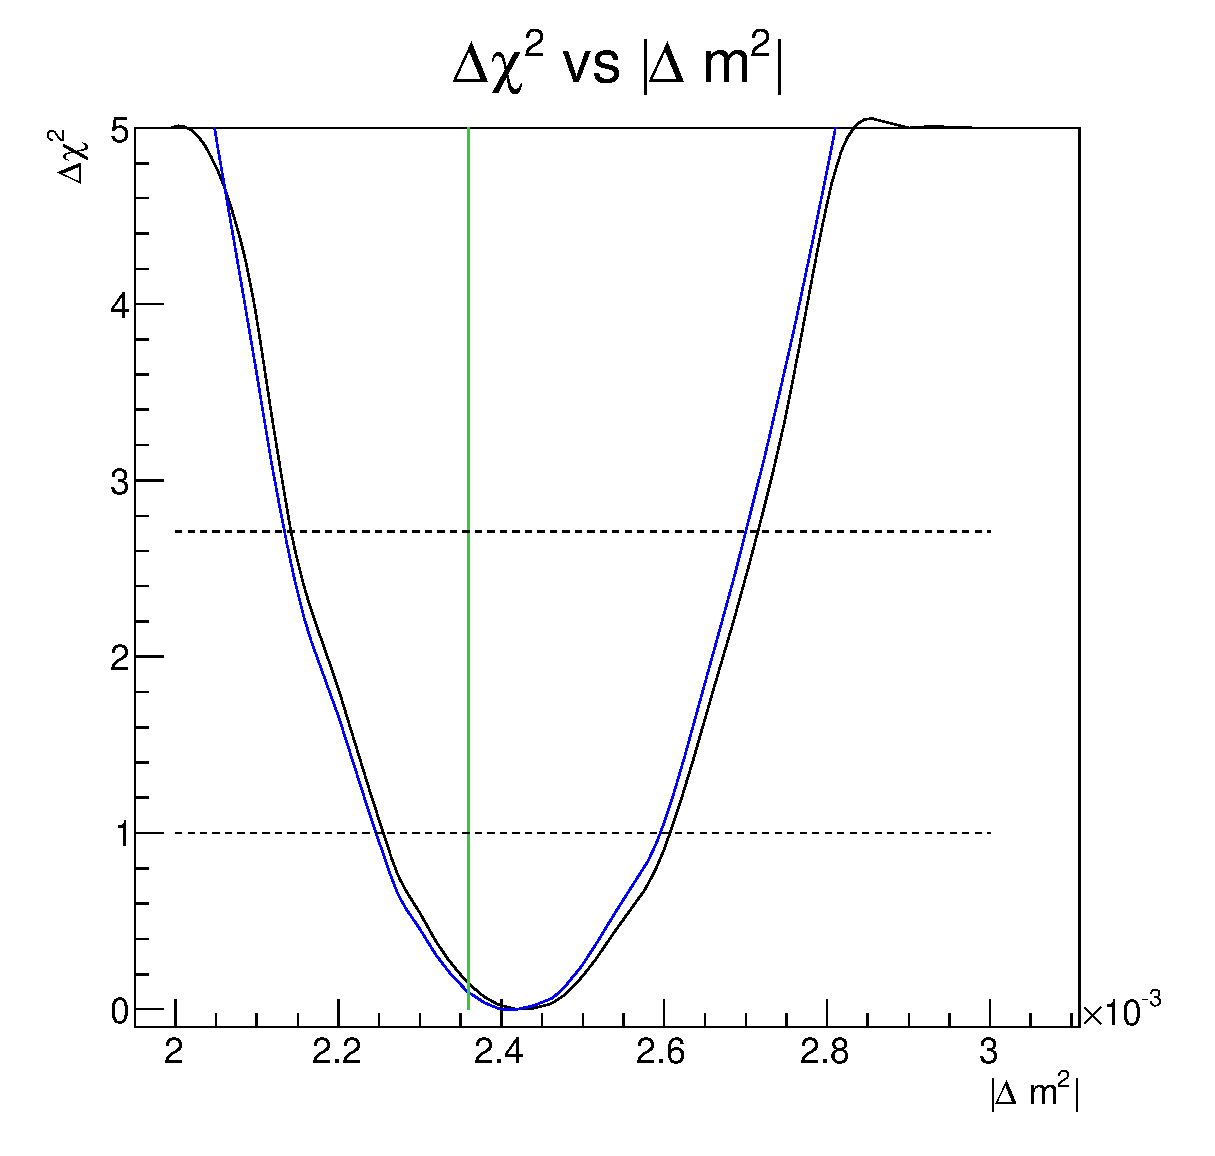
\includegraphics[width=9pc]{./images/appendix/sensitivity_studies/sensitivity_point0_chisq_vs_dm23sq.eps}
\caption {
  $\Delta\chi^2$ as a function of $|\Delta m^{2}|$ for true oscillation parameter point \#0.
  $\chi^2$ was averaged over hundreds of toy-MC experiments and,
  for each experiment, it was minimized with respect to 
  $\sin^{2}\theta_{23}$, $\sin^{2}\theta_{13}$, $\delta_{CP}$
  and all relevant nuisance parameters for the joint analysis (black)
  and with respect to $\sin^{2}\theta_{23}$ and all relevant nuisance
  parameters for the disappearance analysis (blue).
  }
\label{fig:sensitivity:point0:dchisq_Dmsq}
\end{minipage}
\hspace{0.02\linewidth}
\begin{minipage}[t]{0.22\linewidth}
\center
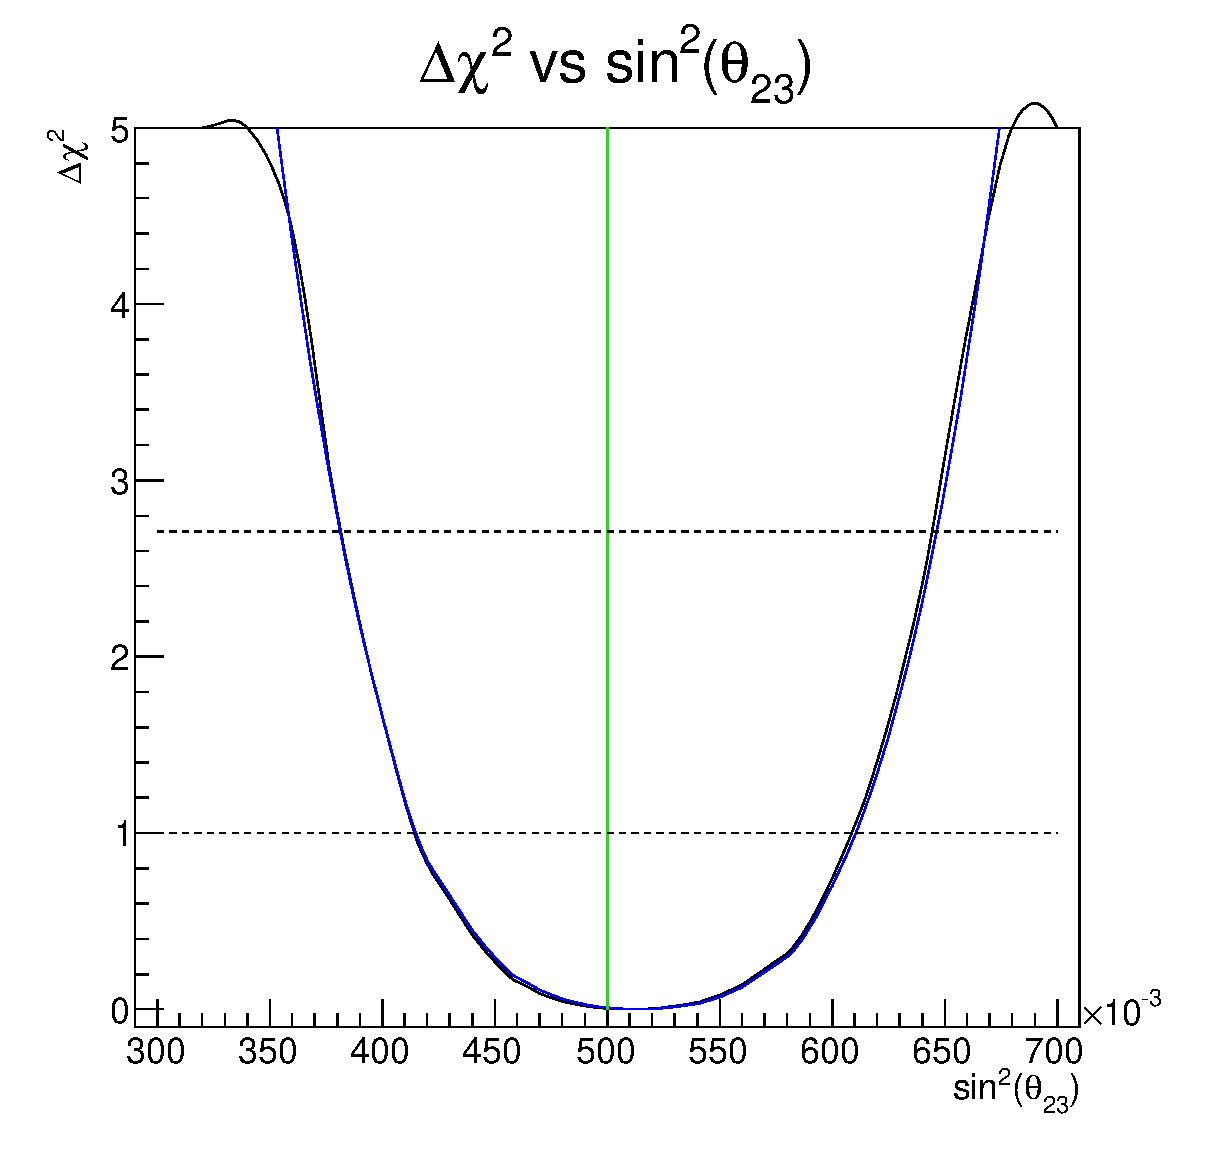
\includegraphics[width=9pc]{./images/appendix/sensitivity_studies/sensitivity_point0_chisq_vs_theta23.eps}
\caption {
  $\Delta\chi^2$ as function of $\sin^{2}\theta_{23}$ for true oscillation parameter point \#0.
  $\chi^2$ was averaged over hundreds of toy-MC experiments and,
  for each experiment, it was minimized with respect to 
  $\sin^{2}\theta_{23}$, $\sin^{2}\theta_{13}$, $\delta_{CP}$
  and all relevant nuisance parameters for the joint analysis (black)
  and with respect to $\sin^{2}\theta_{23}$ and all relevant nuisance
  parameters for the disappearance analysis (blue).
}
\label{fig:sensitivity:point0:dchisq_sinsqtheta23}
\end{minipage}
\hspace{0.02\linewidth}
\begin{minipage}[t]{0.22\linewidth}
\center
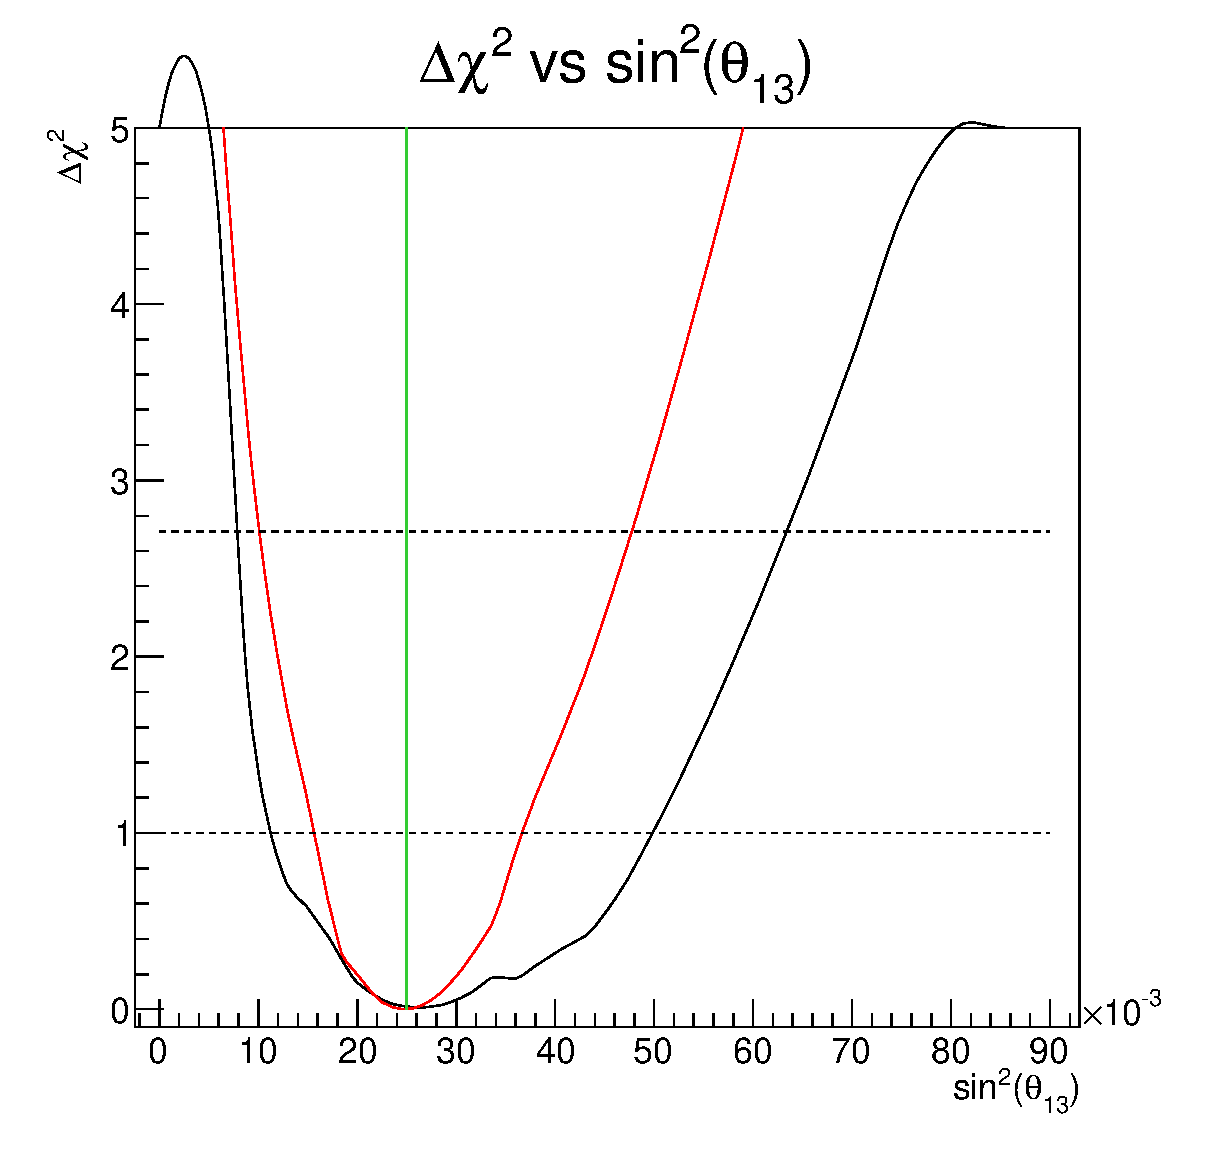
\includegraphics[width=9pc]{./images/appendix/sensitivity_studies/sensitivity_point0_chisq_vs_theta13.eps}
\caption {
  $\Delta\chi^2$ as function of $\sin^{2}\theta_{13}$ for true oscillation parameter point \#0.
  $\chi^2$ was averaged over hundreds of toy-MC experiments and,
  for each experiment, it was minimized with respect to 
  $\sin^{2}\theta_{23}$, $\sin^{2}\theta_{13}$, $\delta_{CP}$
  and all relevant nuisance parameters for the joint analysis (black)
  and with respect to all relevant nuisance parameters 
  ($\delta_{CP}$ is fixed to 0) for the appearance analysis (red).
}
\label{fig:sensitivity:point0:dchisq_sinsqtheta13}
\end{minipage}
\hspace{0.02\linewidth}
\begin{minipage}[t]{0.22\linewidth}
\center
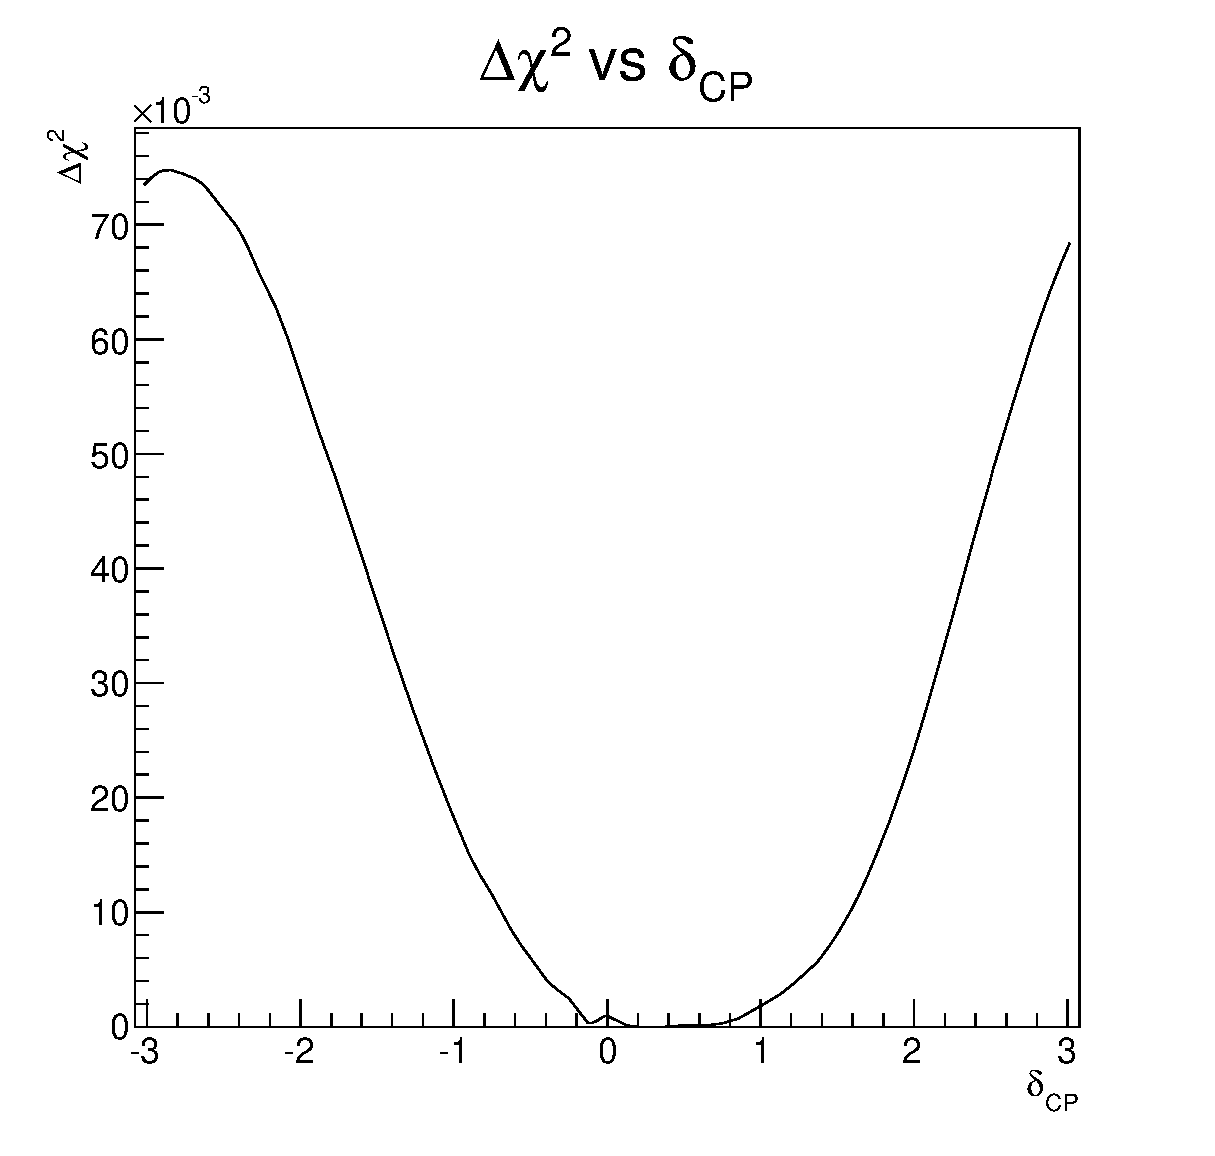
\includegraphics[width=9pc]{./images/appendix/sensitivity_studies/sensitivity_point0_chisq_vs_deltacp.eps}
\caption {
  $\Delta\chi^2$ as function of $\delta_{CP}$ for true oscillation parameter point \#0.
  $\chi^2$ was averaged over hundreds of toy-MC experiments and,
  for each experiment, it was minimized with respect to 
  $|\Delta m^{2}|$, $\sin^{2}\theta_{23}$, $\sin^{2}\theta_{13}$
  and all relevant nuisance parameters.
}
\label{fig:sensitivity:point0:dchisq_deltacp}
\end{minipage}


\end{figure*}



%
% ..............................................................................
% delta\chisq and contours - true point 1
%

\begin{figure*}[htb]

\begin{minipage}[t]{0.22\linewidth}
\center
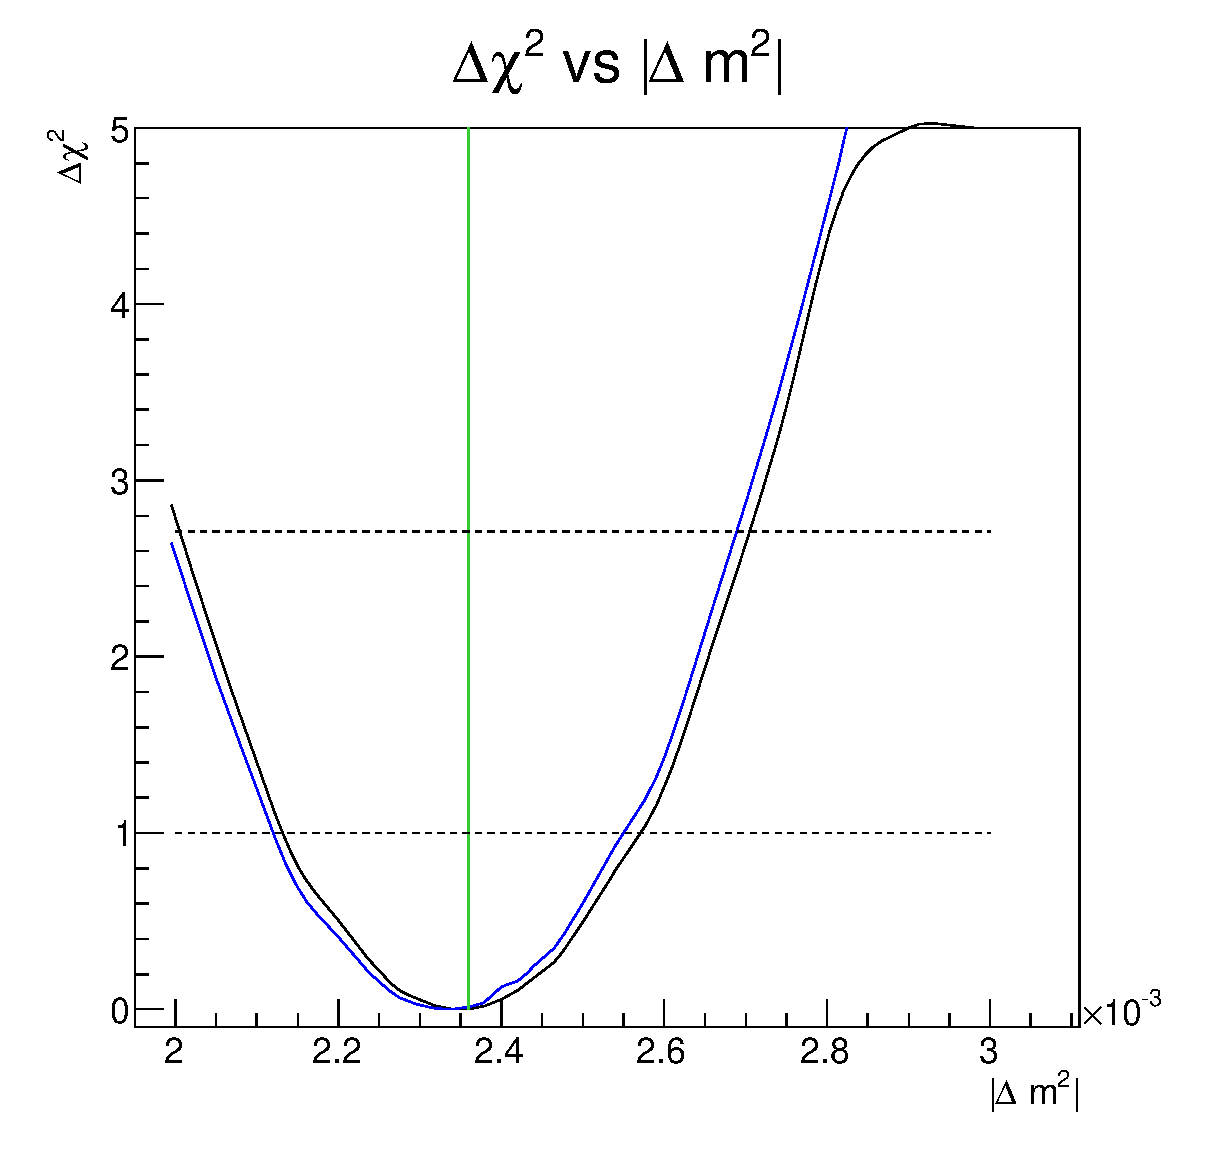
\includegraphics[width=9pc]{./images/appendix/sensitivity_studies/sensitivity_point1_chisq_vs_dm23sq.eps}
\caption {
  $\Delta\chi^2$ as function of $|\Delta m^{2}|$ for true oscillation parameter point \#1.
  $\chi^2$ was averaged over hundreds of toy-MC experiments and,
  for each experiment, it was minimized with respect to 
  $\sin^{2}\theta_{23}$, $\sin^{2}\theta_{13}$, $\delta_{CP}$
  and all relevant nuisance parameters for the joint analysis (black)
  and with respect to $\sin^{2}\theta_{23}$ and all relevant nuisance
  parameters for the disappearance analysis (blue). 
}
\label{fig:sensitivity:point1:dchisq_Dmsq}
\end{minipage}
\hspace{0.02\linewidth}
\begin{minipage}[t]{0.22\linewidth}
\center
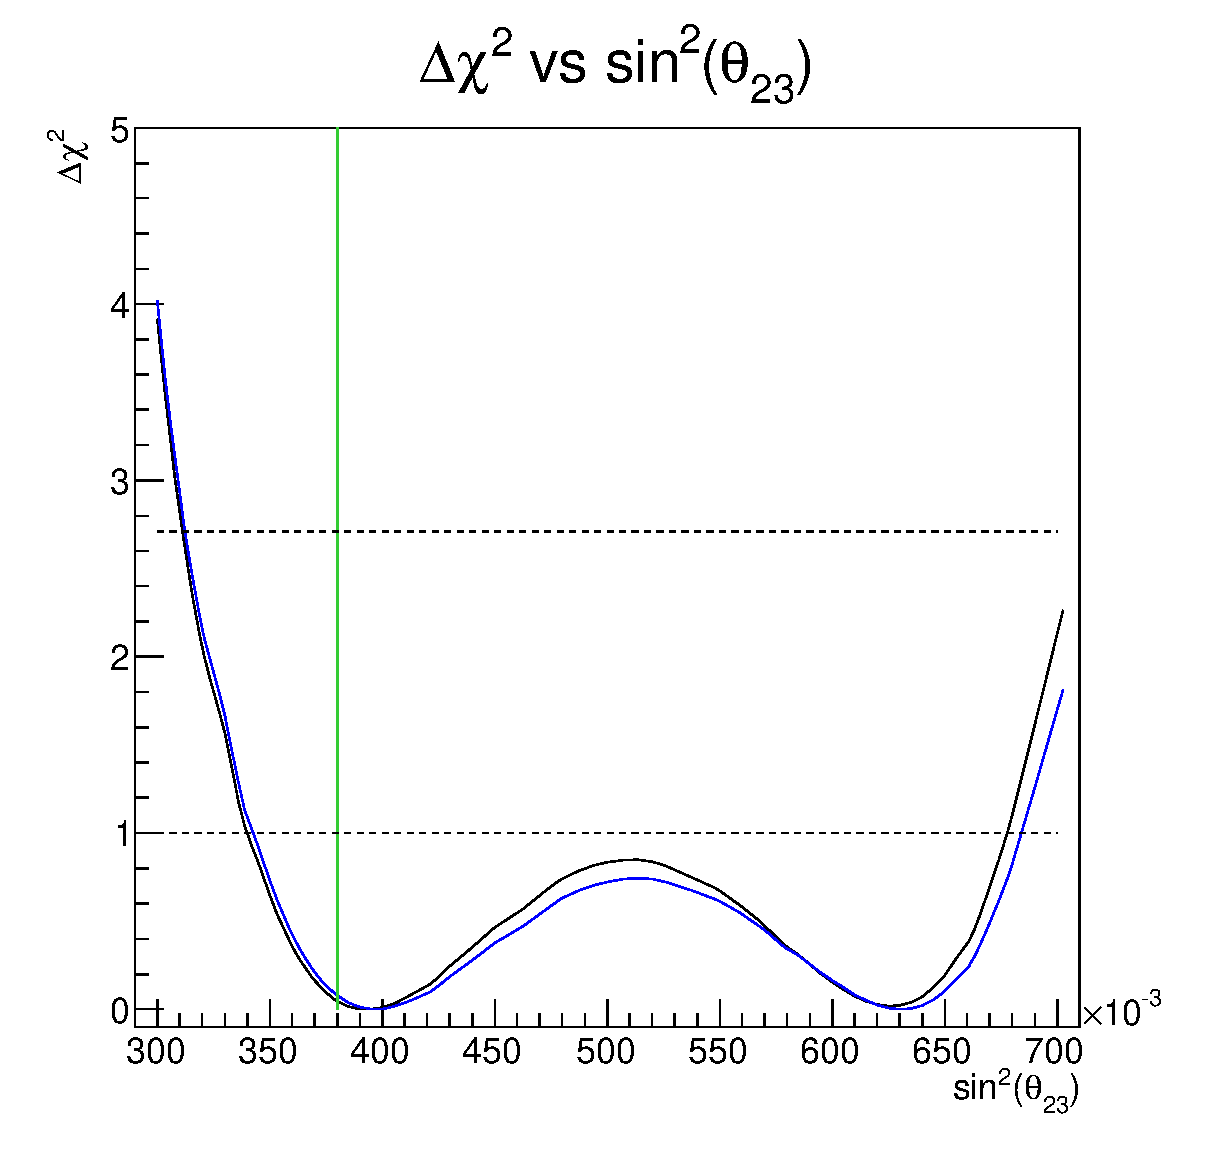
\includegraphics[width=9pc]{./images/appendix/sensitivity_studies/sensitivity_point1_chisq_vs_theta23.eps}
\caption {
  $\Delta\chi^2$ as function of $\sin^{2}\theta_{23}$ for true oscillation parameter point \#1.
  $\chi^2$ was averaged over hundreds of toy-MC experiments and,
  for each experiment, it was minimized with respect to 
  $|\Delta m^{2}|$, $\sin^{2}\theta_{13}$, $\delta_{CP}$
  and all relevant nuisance parameters for the joint analysis (black)
  and with respect to $\sin^{2}\theta_{23}$ and all relevant nuisance
  parameters for the disappearance analysis (blue).
  }
\label{fig:sensitivity:point1:dchisq_sinsqtheta23}
\end{minipage}
\hspace{0.02\linewidth}
\begin{minipage}[t]{0.22\linewidth}
\center
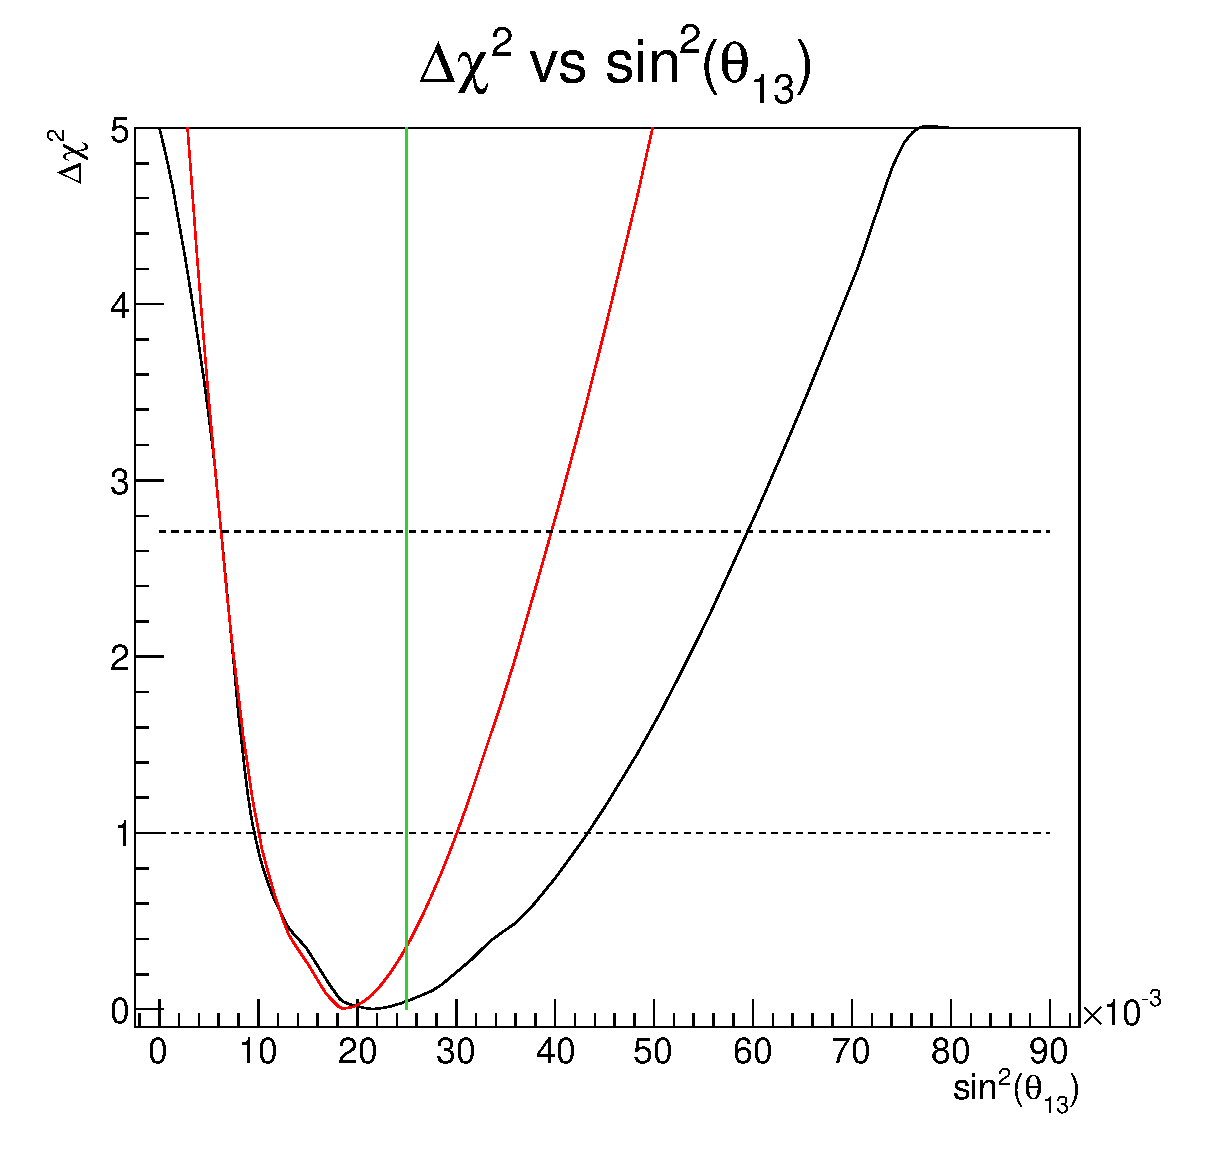
\includegraphics[width=9pc]{./images/appendix/sensitivity_studies/sensitivity_point1_chisq_vs_theta13.eps}
\caption {
  $\Delta\chi^2$ as function of $\sin^{2}\theta_{13}$ for true oscillation parameter point \#1.
  $\chi^2$ was averaged over hundreds of toy-MC experiments and,
  for each experiment, it was minimized with respect to 
  $\sin^{2}\theta_{23}$, $\sin^{2}\theta_{13}$, $\delta_{CP}$
  and all relevant nuisance parameters for the joint analysis (black)
  and with respect to all relevant nuisance parameters 
  ($\delta_{CP}$ is fixed to 0) for the appearance analysis (red).
}
\label{fig:sensitivity:point1:dchisq_sinsqtheta13}
\end{minipage}
\hspace{0.02\linewidth}
\begin{minipage}[t]{0.22\linewidth}
\center
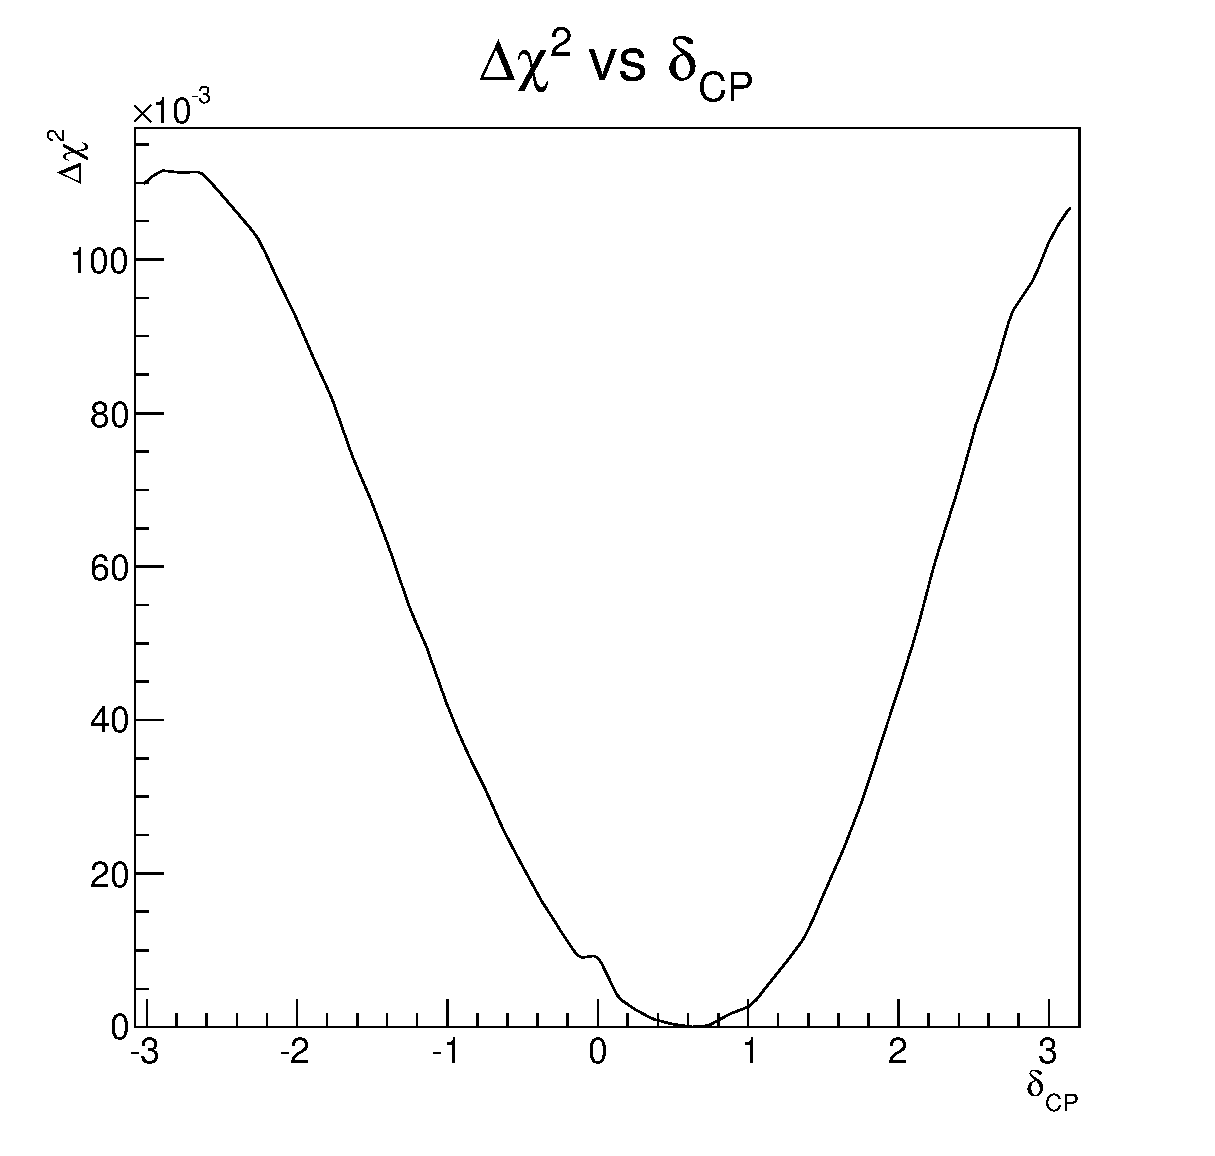
\includegraphics[width=9pc]{./images/appendix/sensitivity_studies/sensitivity_point1_chisq_vs_deltacp.eps}
\caption {
  $\Delta\chi^2$ as function of $\delta_{CP}$ for true oscillation parameter point \#1.
  $\chi^2$ was averaged over hundreds of toy-MC experiments and,
  for each experiment, it was minimized with respect to 
  $|\Delta m^{2}|$, $\sin^{2}\theta_{23}$, $\sin^{2}\theta_{13}$
  and all relevant nuisance parameters.
}
\label{fig:sensitivity:point1:dchisq_deltacp}
\end{minipage}

\end{figure*}


%
% ..............................................................................
% delta\chisq and contours - true point 2
%

\begin{figure*}[htb]

\begin{minipage}[t]{0.22\linewidth}
\center
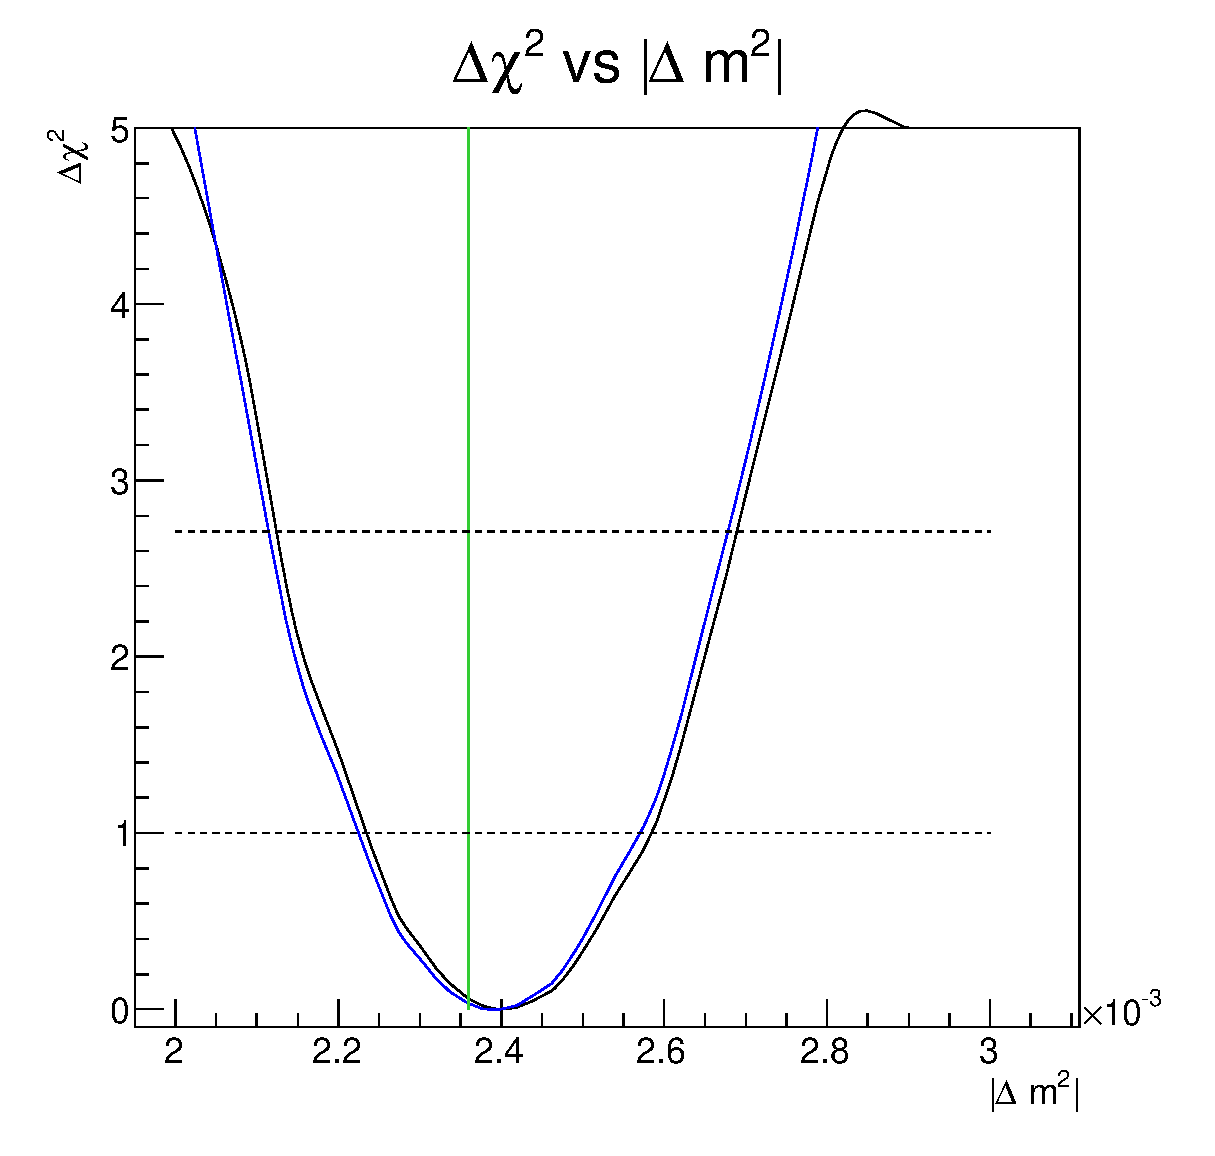
\includegraphics[width=9pc]{./images/appendix/sensitivity_studies/sensitivity_point3_chisq_vs_dm23sq.eps}
\caption {
  $\Delta\chi^2$ as function of $|\Delta m^{2}|$ for true oscillation parameter point \#2.
  $\chi^2$ was averaged over hundreds of toy-MC experiments and,
  for each experiment, it was minimized with respect to 
  $\sin^{2}\theta_{23}$, $\sin^{2}\theta_{13}$, $\delta_{CP}$
  and all relevant nuisance parameters for the joint analysis (black)
  and with respect to $\sin^{2}\theta_{23}$ and all relevant nuisance
  parameters for the disappearance analysis (blue).
  }
\label{fig:sensitivity:point2:dchisq_Dmsq}
\end{minipage}
\hspace{0.02\linewidth}
\begin{minipage}[t]{0.22\linewidth}
\center
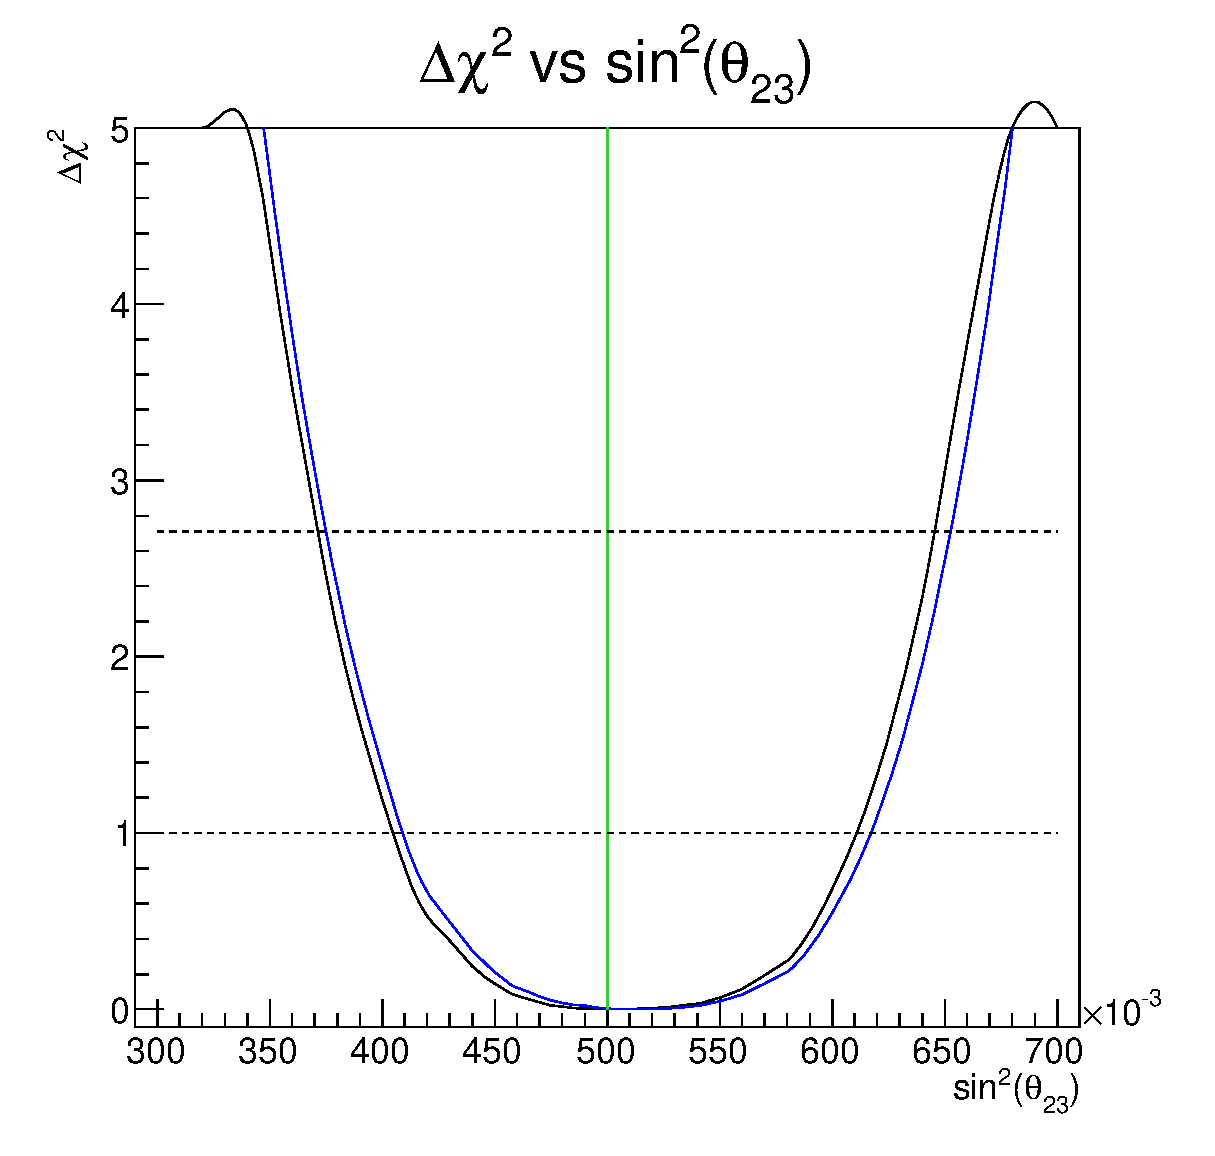
\includegraphics[width=9pc]{./images/appendix/sensitivity_studies/sensitivity_point3_chisq_vs_theta23.eps}
\caption {
  $\Delta\chi^2$ as function of $\sin^{2}\theta_{23}$ for true oscillation parameter point \#2.
  $\chi^2$ was averaged over hundreds of toy-MC experiments and,
  for each experiment, it was minimized with respect to 
  $|\Delta m^{2}|$, $\sin^{2}\theta_{13}$, $\delta_{CP}$
  and all relevant nuisance parameters for the joint analysis (black)
  and with respect to $\sin^{2}\theta_{23}$ and all relevant nuisance
  parameters for the disappearance analysis (blue).
}
\label{fig:sensitivity:point2:dchisq_sinsqtheta23}
\end{minipage}
\hspace{0.02\linewidth}
\begin{minipage}[t]{0.22\linewidth}
\center
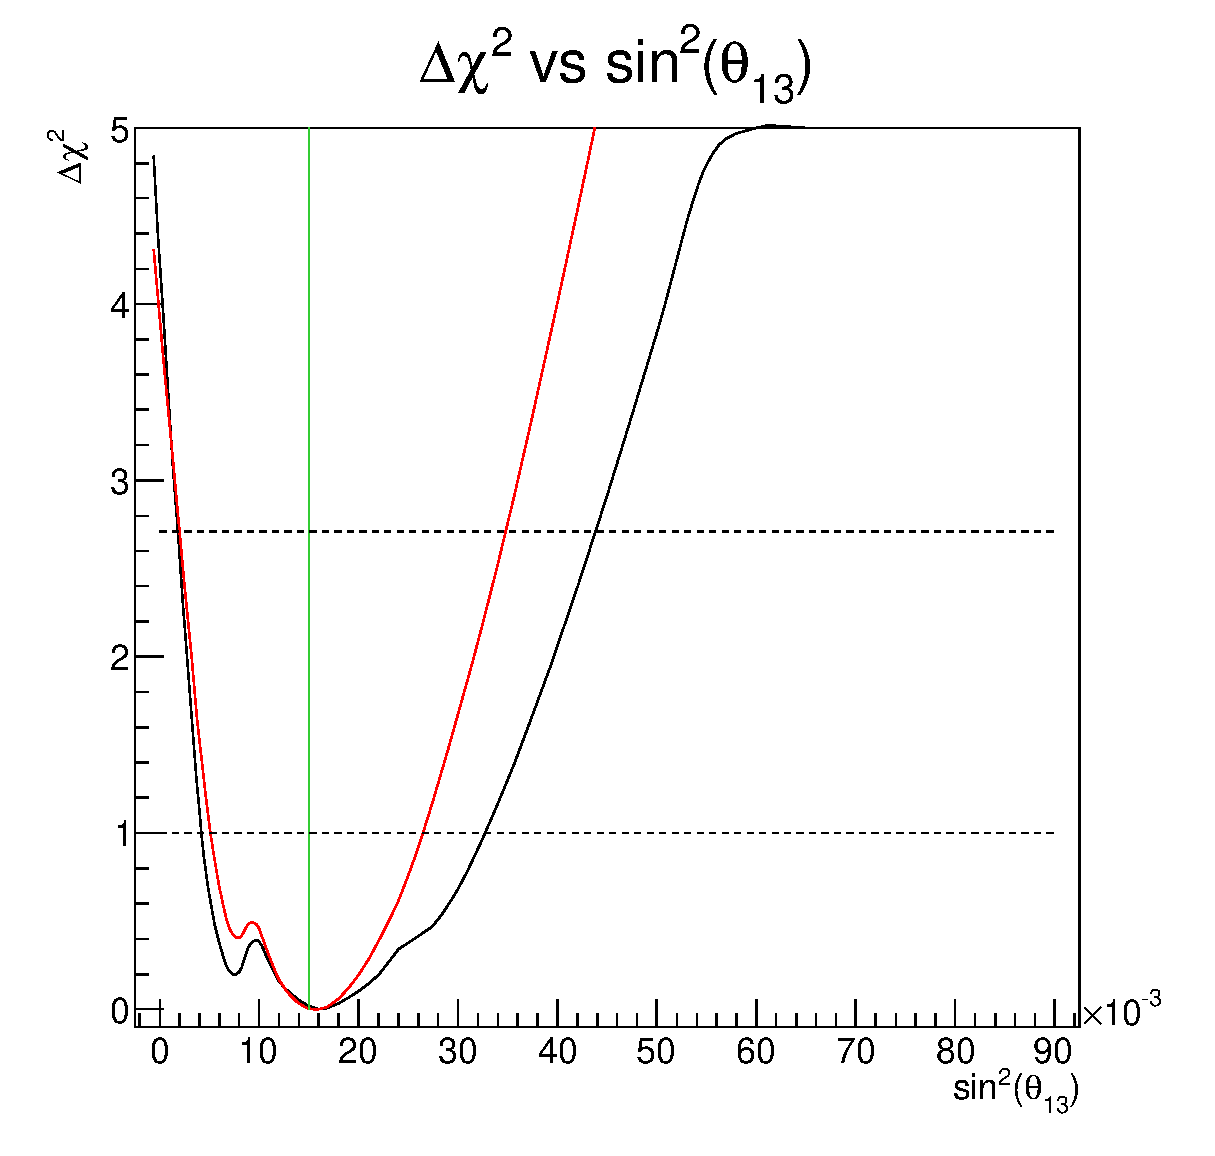
\includegraphics[width=9pc]{./images/appendix/sensitivity_studies/sensitivity_point3_chisq_vs_theta13.eps}
\caption {
  $\Delta\chi^2$ as function of $\sin^{2}\theta_{13}$ for true oscillation parameter point \#2.
  $\chi^2$ was averaged over hundreds of toy-MC experiments and,
  for each experiment, it was minimized with respect to 
  $\sin^{2}\theta_{23}$, $\sin^{2}\theta_{13}$, $\delta_{CP}$
  and all relevant nuisance parameters for the joint analysis (black)
  and with respect to all relevant nuisance parameters 
  ($\delta_{CP}$ is fixed to 0) for the appearance analysis (red).
}
\label{fig:sensitivity:point2:dchisq_sinsqtheta13}
\end{minipage}
\hspace{0.02\linewidth}
\begin{minipage}[t]{0.22\linewidth}
\center
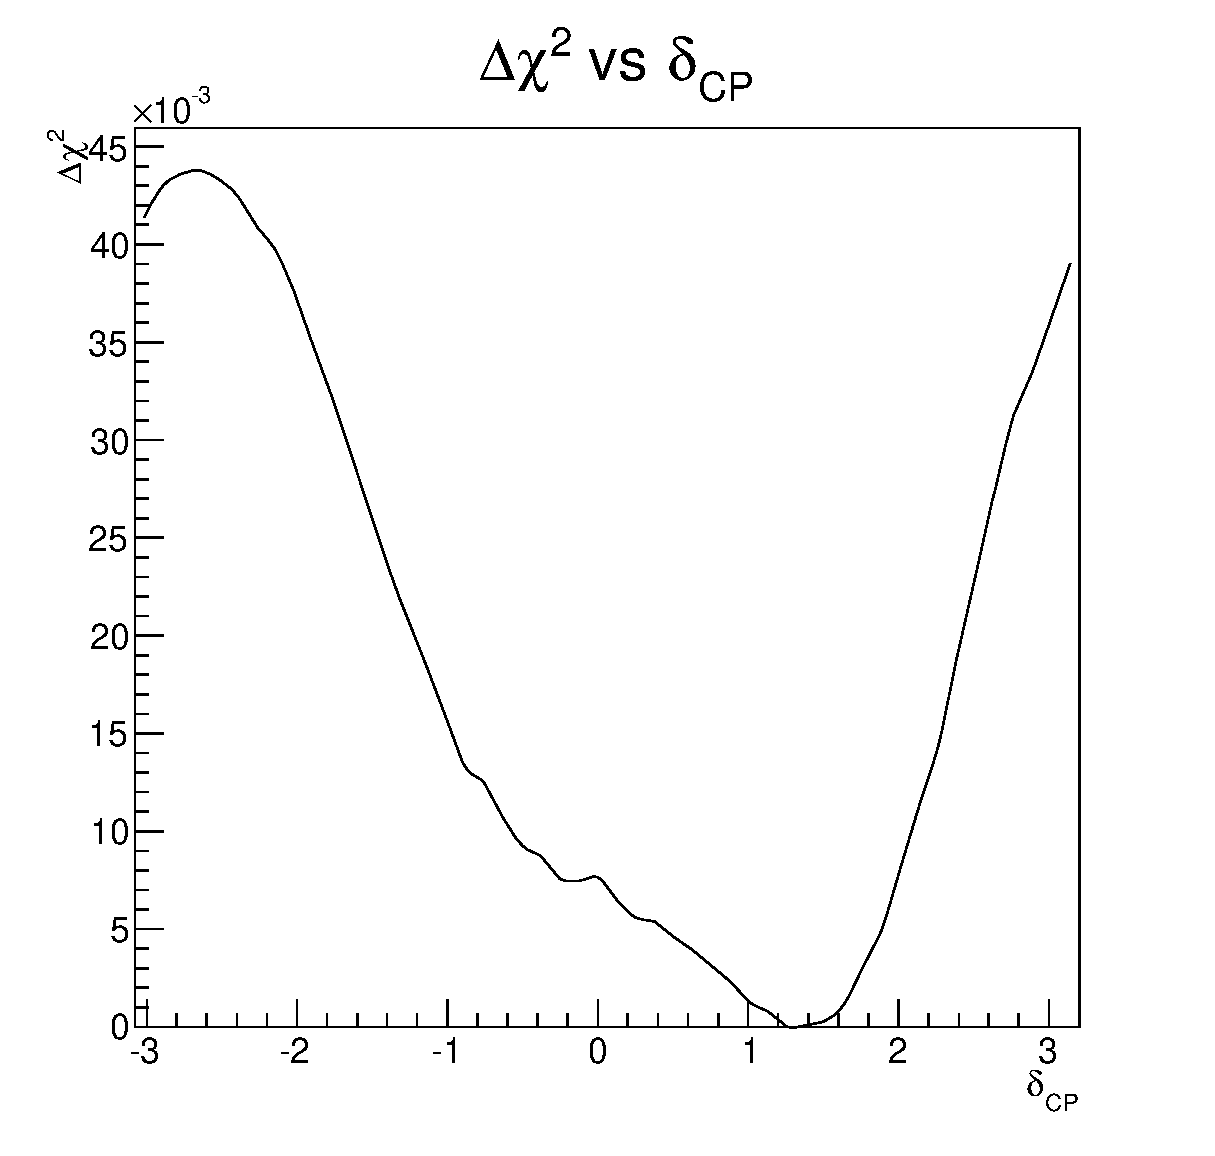
\includegraphics[width=9pc]{./images/appendix/sensitivity_studies/sensitivity_point3_chisq_vs_deltacp.eps}
\caption {
  $\Delta\chi^2$ as function of $\delta_{CP}$ for true oscillation parameter point \#2.
  $\chi^2$ was averaged over hundreds of toy-MC experiments and,
  for each experiment, it was minimized with respect to 
  $|\Delta m^{2}|$, $\sin^{2}\theta_{23}$, $\sin^{2}\theta_{13}$
  and all relevant nuisance parameters.
}
\label{fig:sensitivity:point2:dchisq_deltacp}
\end{minipage}

\end{figure*}



%
% ..............................................................................
% delta\chisq and contours - true point 3
%

\begin{figure*}[htb]

\begin{minipage}[t]{0.22\linewidth}
\center
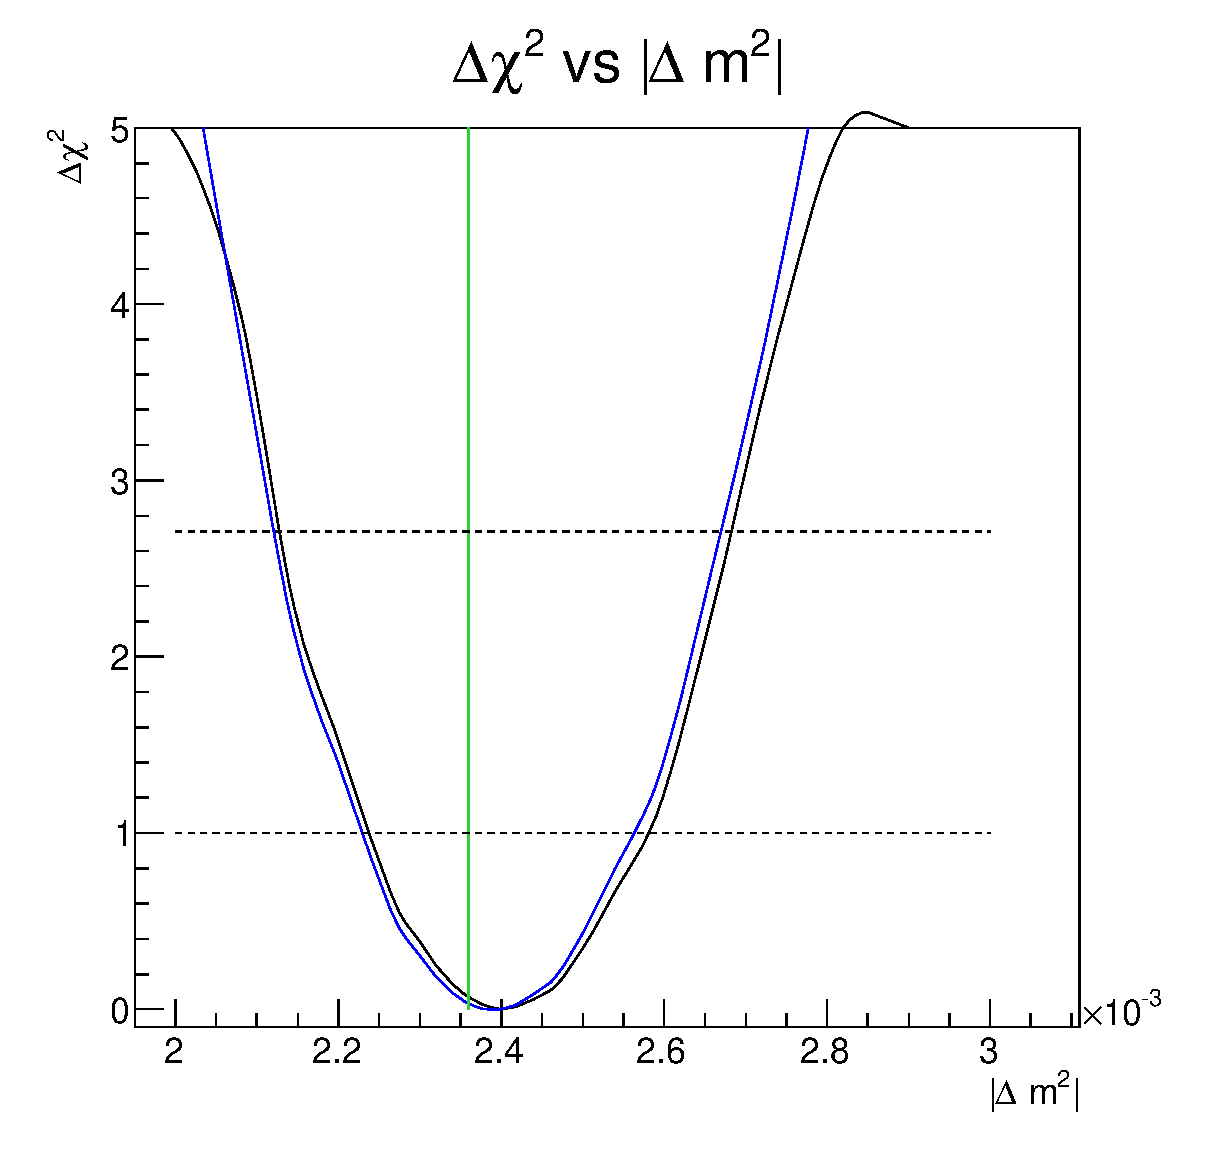
\includegraphics[width=9pc]{./images/appendix/sensitivity_studies/sensitivity_point5_chisq_vs_dm23sq.eps}
\caption {
  $\Delta\chi^2$ as function of $|\Delta m^{2}|$ for true oscillation parameter point \#3.
 $\chi^2$ was averaged over hundreds of toy-MC experiments and,
  for each experiment, it was minimized with respect to 
  $\sin^{2}\theta_{23}$, $\sin^{2}\theta_{13}$, $\delta_{CP}$
  and all relevant nuisance parameters for the joint analysis (black)
  and with respect to $\sin^{2}\theta_{23}$ and all relevant nuisance
  parameters for the disappearance analysis (blue).
}
\label{fig:sensitivity:point3:dchisq_Dmsq}
\end{minipage}
\hspace{0.02\linewidth}
\begin{minipage}[t]{0.22\linewidth}
\center
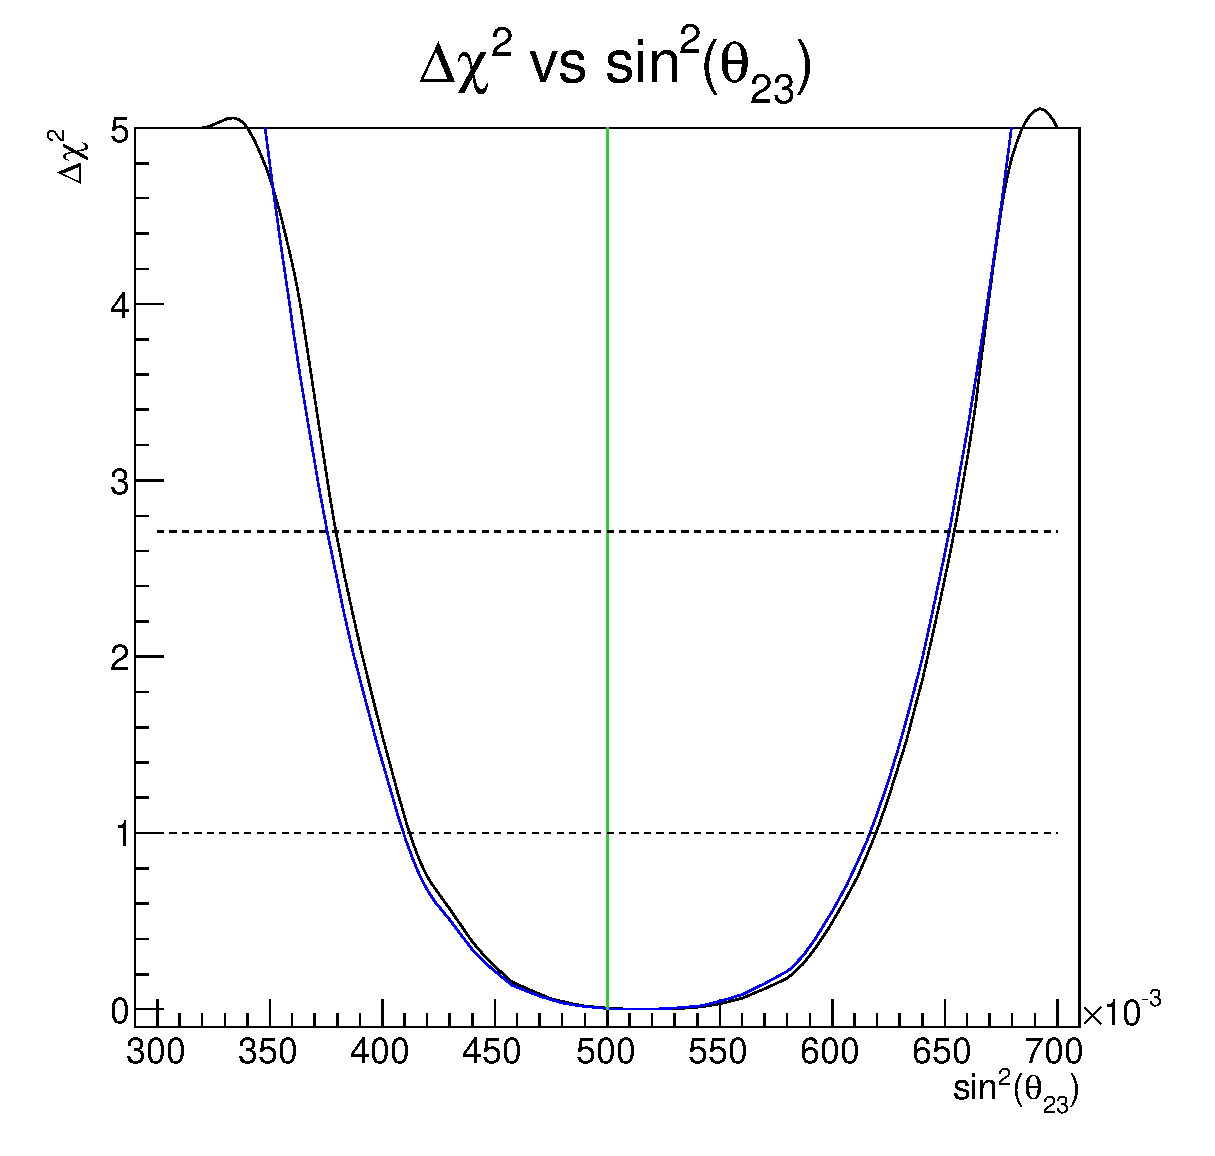
\includegraphics[width=9pc]{./images/appendix/sensitivity_studies/sensitivity_point5_chisq_vs_theta23.eps}
\caption {
  $\Delta\chi^2$ as function of $\sin^{2}\theta_{23}$ for true oscillation parameter point \#3.
 $\chi^2$ was averaged over hundreds of toy-MC experiments and,
  for each experiment, it was minimized with respect to 
  $|\Delta m^{2}|$, $\sin^{2}\theta_{13}$, $\delta_{CP}$
  and all relevant nuisance parameters for the joint analysis (black)
  and with respect to $\sin^{2}\theta_{23}$ and all relevant nuisance
  parameters for the disappearance analysis (blue).
}
\label{fig:sensitivity:point3:dchisq_sinsqtheta23}
\end{minipage}
\hspace{0.02\linewidth}
\begin{minipage}[t]{0.22\linewidth}
\center
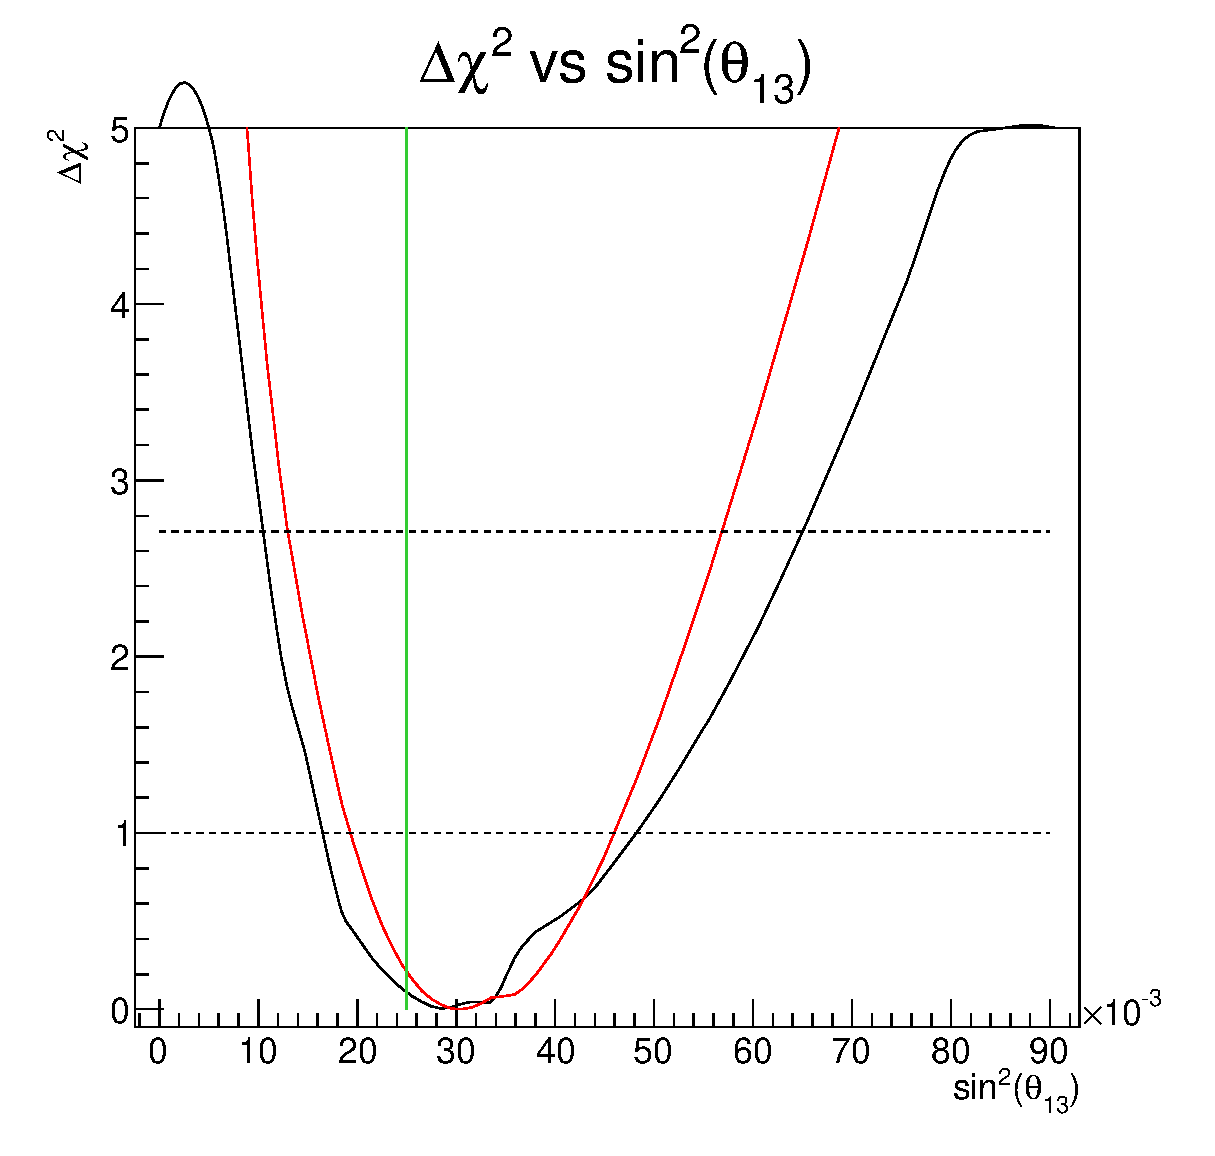
\includegraphics[width=9pc]{./images/appendix/sensitivity_studies/sensitivity_point5_chisq_vs_theta13.eps}
\caption {
  $\Delta\chi^2$ as function of $\sin^{2}\theta_{13}$ for true oscillation parameter point \#3.
  $\chi^2$ was averaged over hundreds of toy-MC experiments and,
  for each experiment, it was minimized with respect to 
  $\sin^{2}\theta_{23}$, $\sin^{2}\theta_{13}$, $\delta_{CP}$
  and all relevant nuisance parameters for the joint analysis (black)
  and with respect to all relevant nuisance parameters 
  ($\delta_{CP}$ is fixed to 0) for the appearance analysis (red).
}
\label{fig:sensitivity:point3:dchisq_sinsqtheta13}
\end{minipage}
\hspace{0.02\linewidth}
\begin{minipage}[t]{0.22\linewidth}
\center
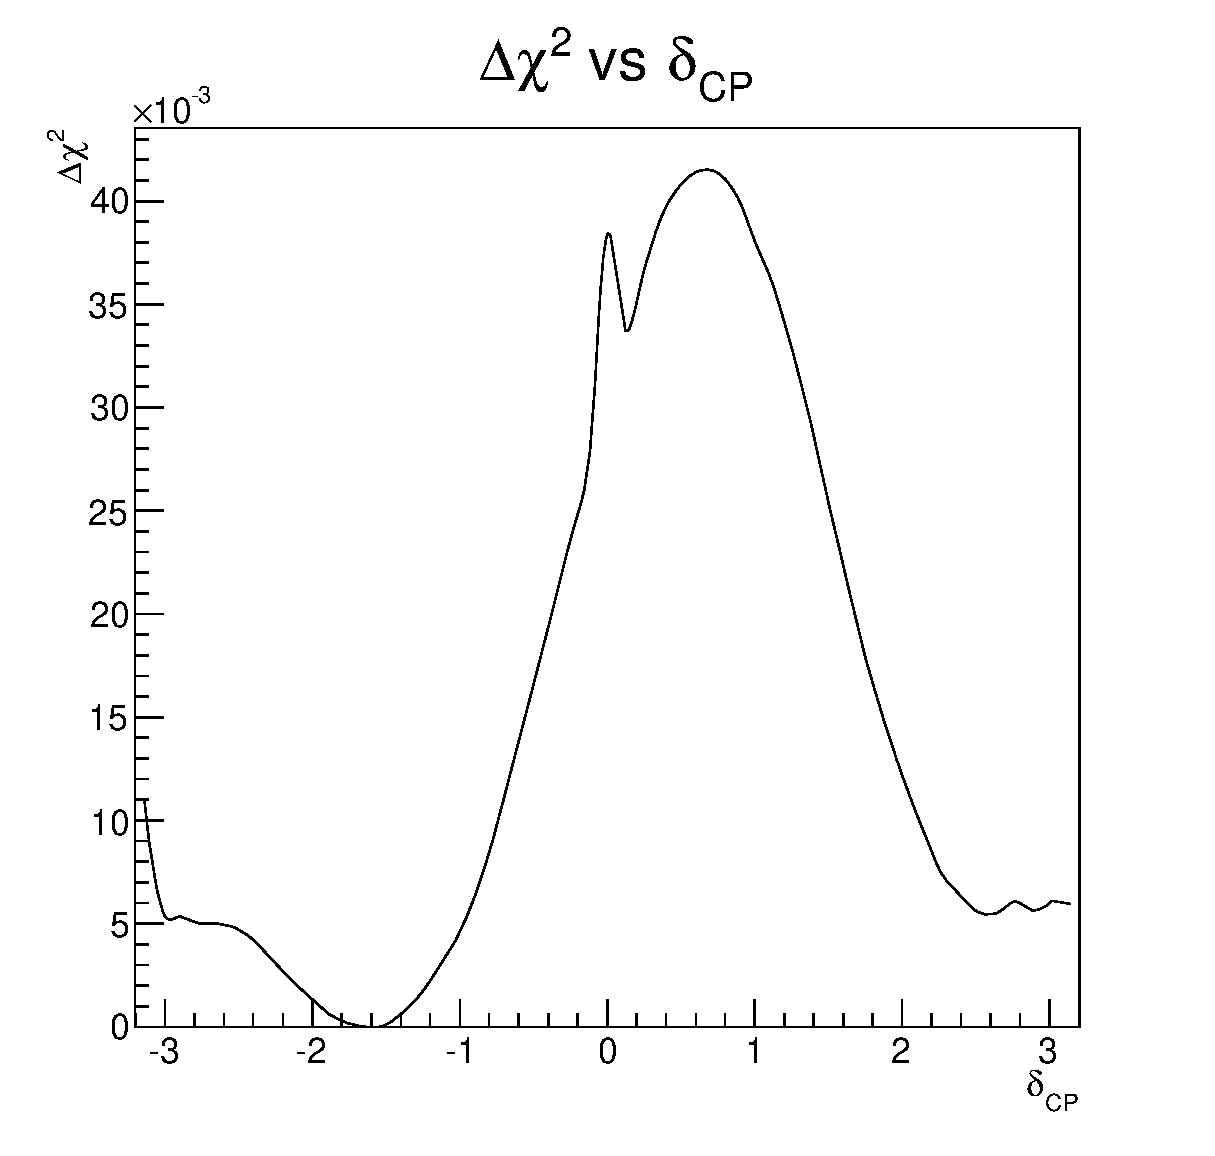
\includegraphics[width=9pc]{./images/appendix/sensitivity_studies/sensitivity_point5_chisq_vs_deltacp.eps}
\caption {
  $\Delta\chi^2$ as function of $\delta_{CP}$ for true oscillation parameter point \#3.
  $\chi^2$ was averaged over hundreds of toy-MC experiments and,
  for each experiment, it was minimized with respect to 
  $|\Delta m^{2}|$, $\sin^{2}\theta_{23}$, $\sin^{2}\theta_{13}$
  and all relevant nuisance parameters.
}
\label{fig:sensitivity:point3:dchisq_deltacp}
\end{minipage}

\end{figure*}


%
% ..............................................................................
% delta\chisq and contours - true point 4
%

\begin{figure*}[htb]

\begin{minipage}[t]{0.22\linewidth}
\center
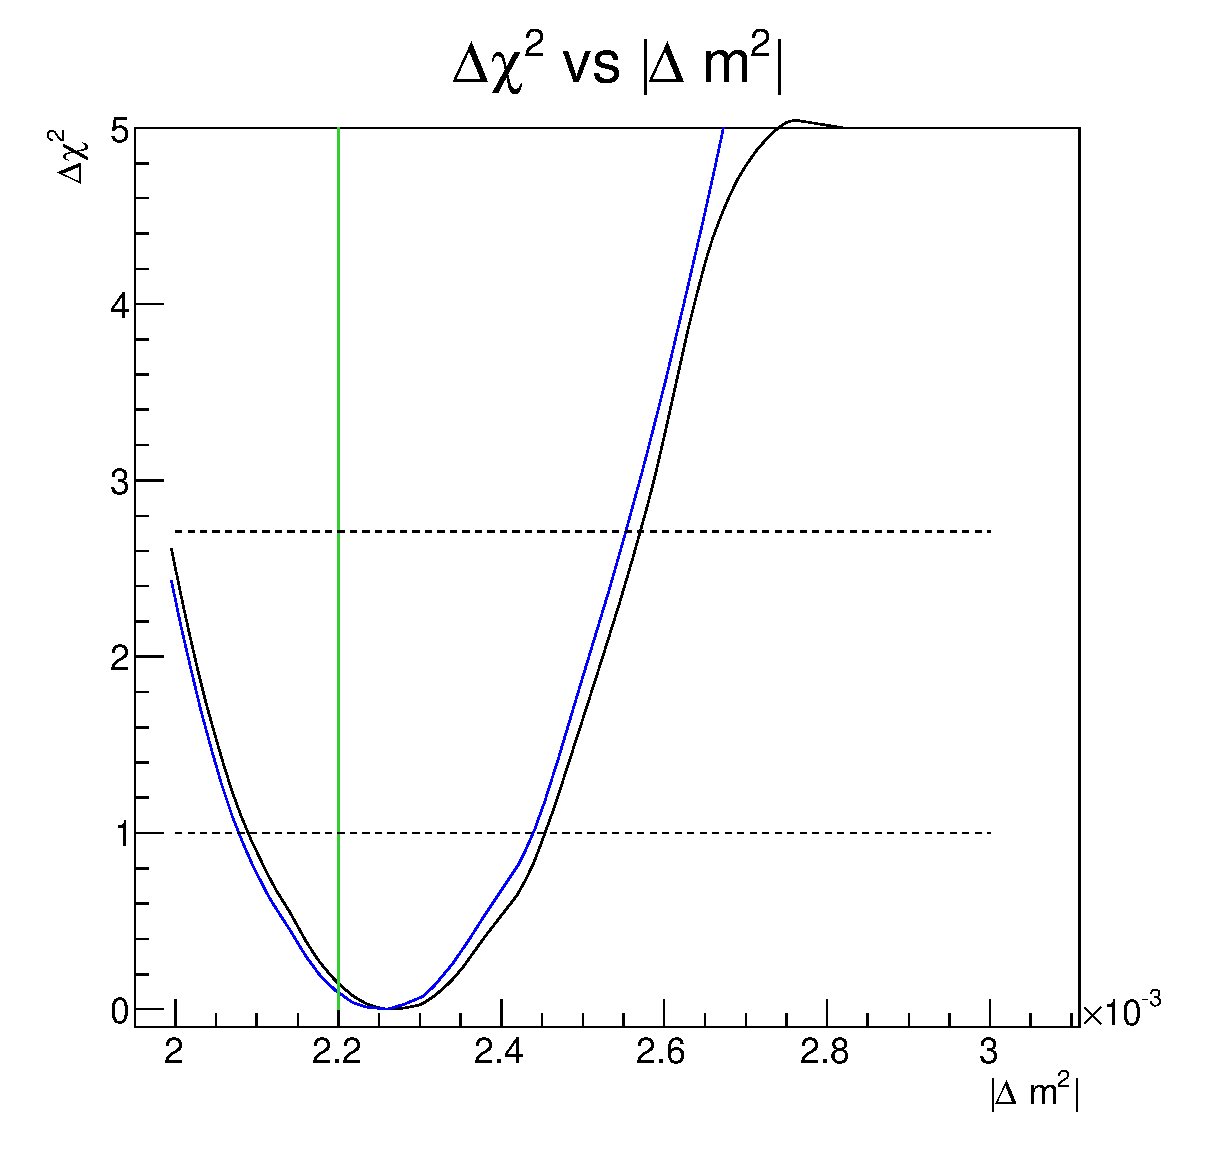
\includegraphics[width=9pc]{./images/appendix/sensitivity_studies/sensitivity_point7_chisq_vs_dm23sq.eps}
\caption {
  $\Delta\chi^2$ as function of $|\Delta m^{2}|$ for true oscillation parameter point \#4.
  $\chi^2$ was averaged over hundreds of toy-MC experiments and,
  for each experiment, it was minimized with respect to 
  $\sin^{2}\theta_{23}$, $\sin^{2}\theta_{13}$, $\delta_{CP}$
  and all relevant nuisance parameters for the joint analysis (black)
  and with respect to $\sin^{2}\theta_{23}$ and all relevant nuisance
  parameters for the disappearance analysis (blue).
  }
\label{fig:sensitivity:point4:dchisq_Dmsq}
\end{minipage}
\hspace{0.02\linewidth}
\begin{minipage}[t]{0.22\linewidth}
\center
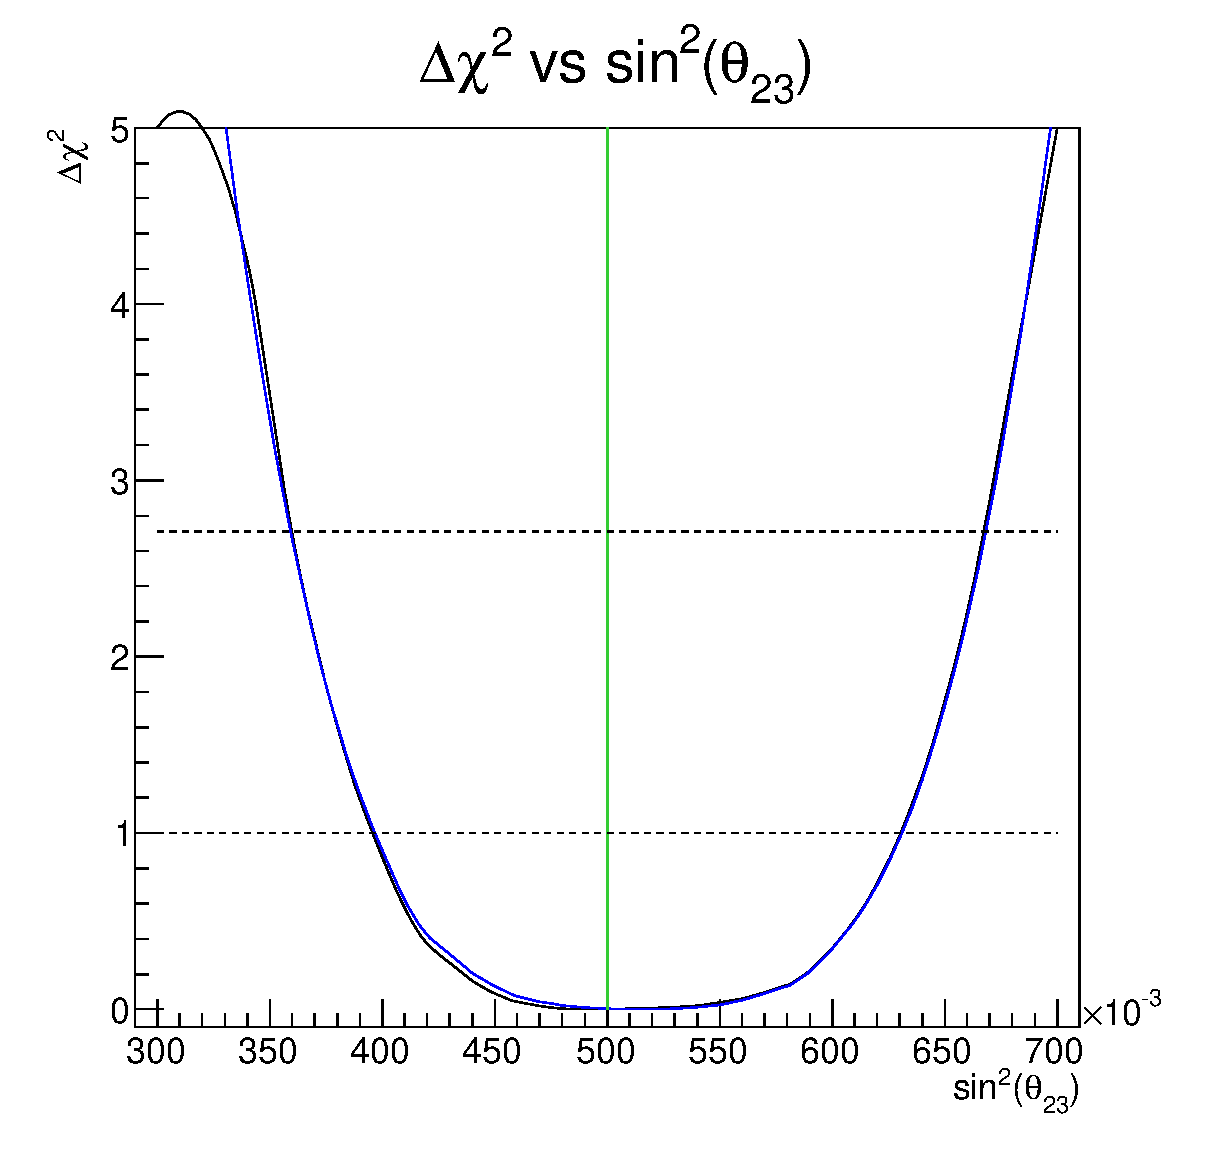
\includegraphics[width=9pc]{./images/appendix/sensitivity_studies/sensitivity_point7_chisq_vs_theta23.eps}
\caption {
  $\Delta\chi^2$ as function of $\sin^{2}\theta_{23}$ for true oscillation parameter point \#4.
  $\chi^2$ was averaged over hundreds of toy-MC experiments and,
  for each experiment, it was minimized with respect to 
  $|\Delta m^{2}|$, $\sin^{2}\theta_{13}$, $\delta_{CP}$
  and all relevant nuisance parameters for the joint analysis (black)
  and with respect to $\sin^{2}\theta_{23}$ and all relevant nuisance
  parameters for the disappearance analysis (blue).
}
\label{fig:sensitivity:point4:dchisq_sinsqtheta23}
\end{minipage}
\hspace{0.02\linewidth}
\begin{minipage}[t]{0.22\linewidth}
\center
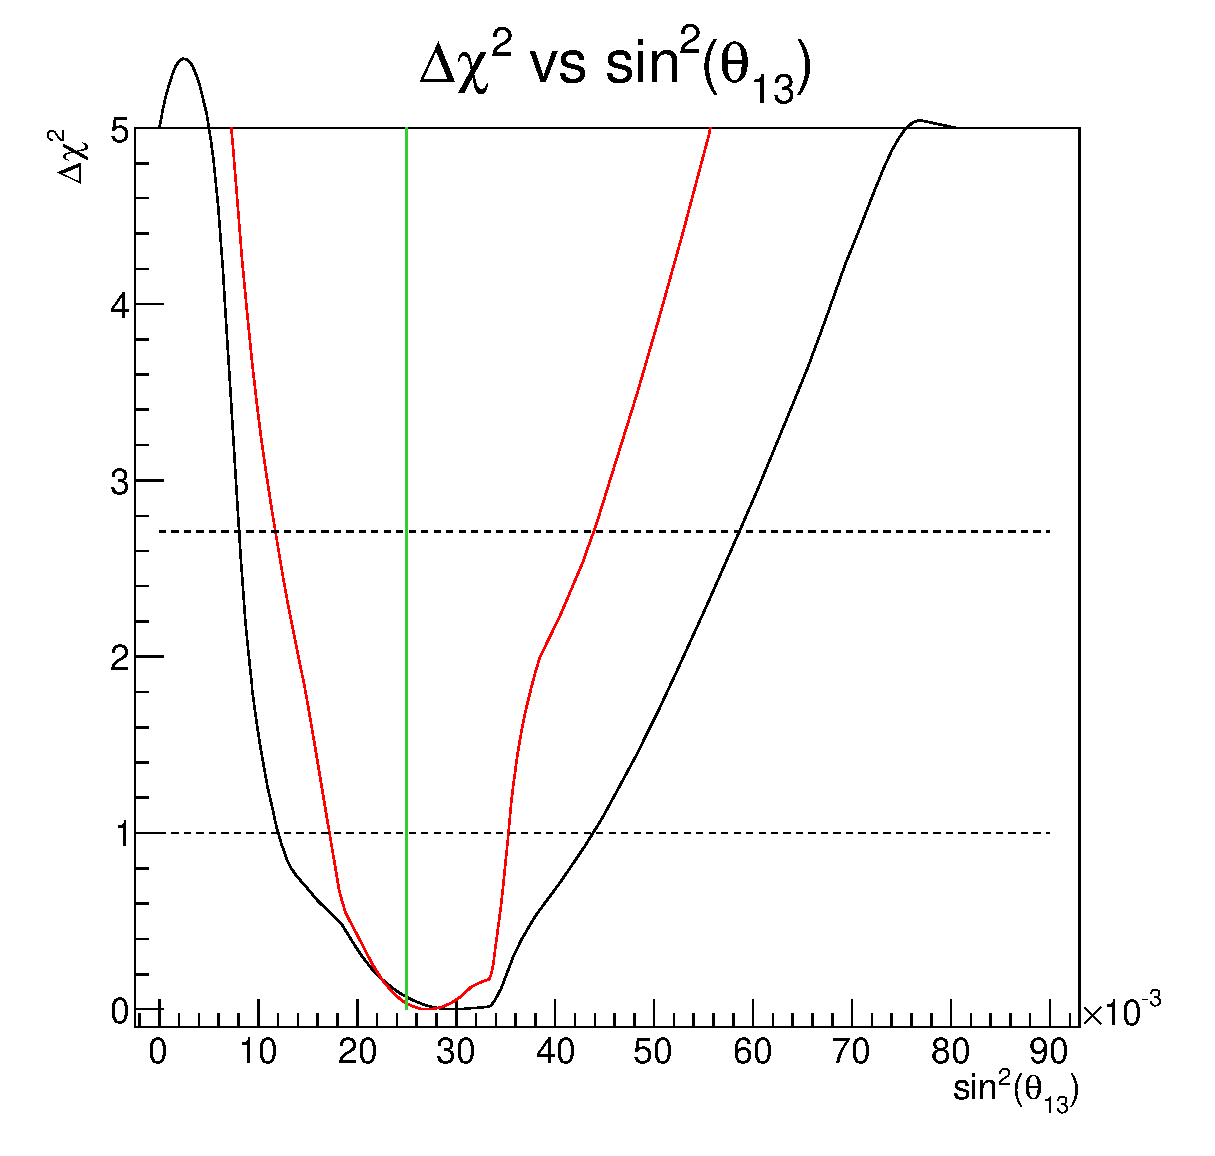
\includegraphics[width=9pc]{./images/appendix/sensitivity_studies/sensitivity_point7_chisq_vs_theta13.eps}
\caption {
  $\Delta\chi^2$ as function of $\sin^{2}\theta_{13}$ for true oscillation parameter point \#4.
  $\chi^2$ was averaged over hundreds of toy-MC experiments and,
  for each experiment, it was minimized with respect to 
  $\sin^{2}\theta_{23}$, $\sin^{2}\theta_{13}$, $\delta_{CP}$
  and all relevant nuisance parameters for the joint analysis (black)
  and with respect to all relevant nuisance parameters 
  ($\delta_{CP}$ is fixed to 0) for the appearance analysis (red).
}
\label{fig:sensitivity:point4:dchisq_sinsqtheta13}
\end{minipage}
\hspace{0.02\linewidth}
\begin{minipage}[t]{0.22\linewidth}
\center
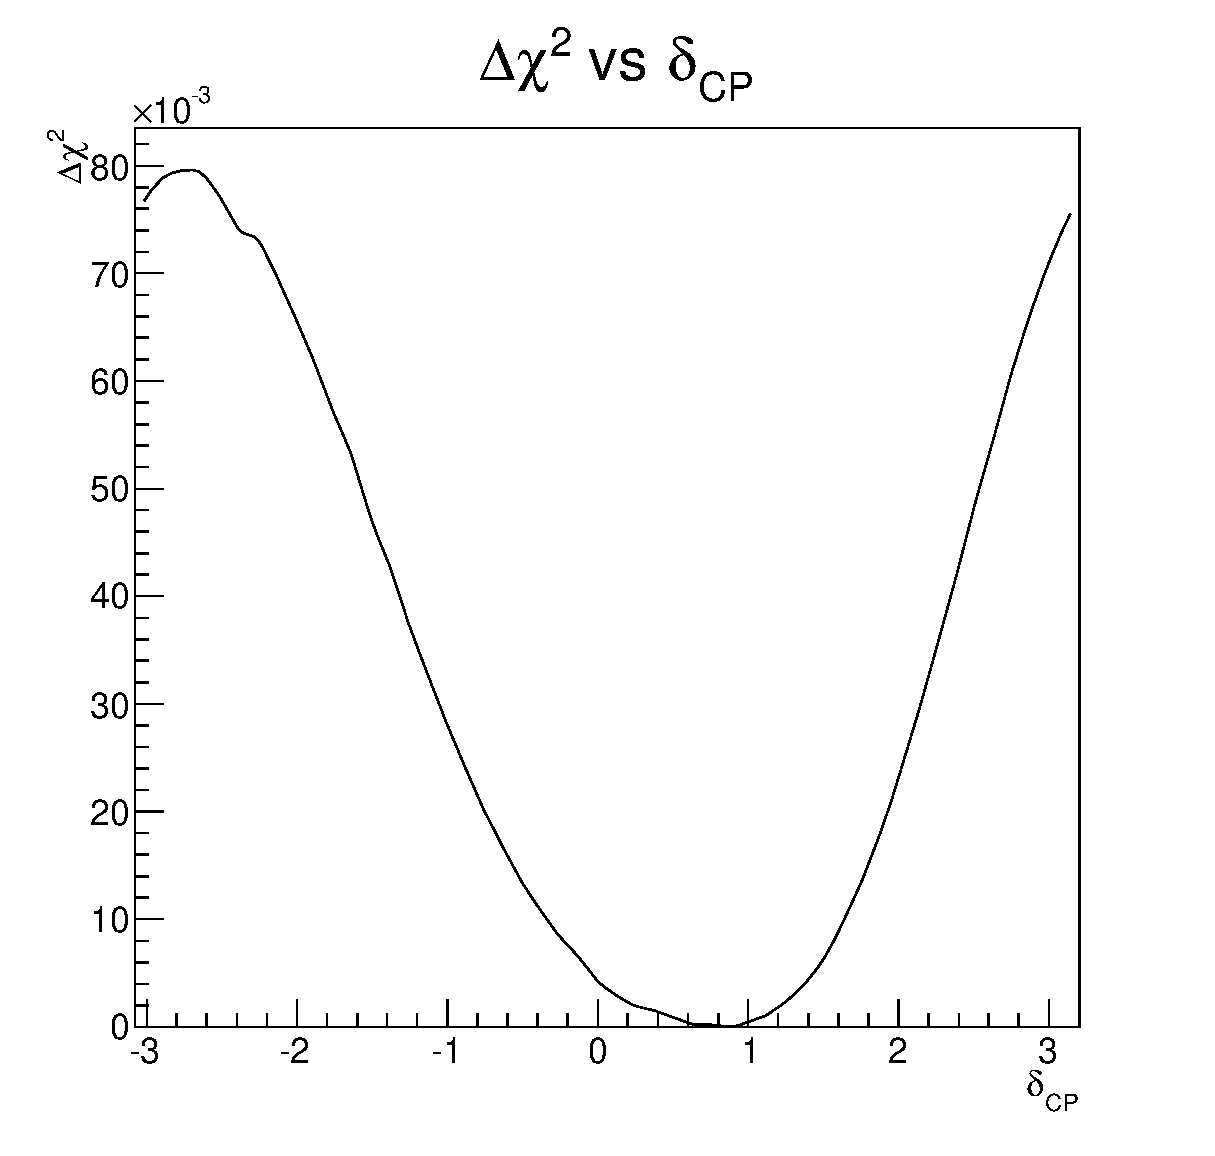
\includegraphics[width=9pc]{./images/appendix/sensitivity_studies/sensitivity_point7_chisq_vs_deltacp.eps}
\caption {
  $\Delta\chi^2$ as function of $\delta_{CP}$ for true oscillation parameter point \#4.
  $\chi^2$ was averaged over hundreds of toy-MC experiments and,
  for each experiment, it was minimized with respect to 
  $|\Delta m^{2}|$, $\sin^{2}\theta_{23}$, $\sin^{2}\theta_{13}$
  and all relevant nuisance parameters.
}
\label{fig:sensitivity:point4:dchisq_deltacp}
\end{minipage}

\end{figure*}

%
% ..............................................................................
% delta\chisq and contours - true point 5
%

\begin{figure*}[htb]

\begin{minipage}[t]{0.22\linewidth}
\center
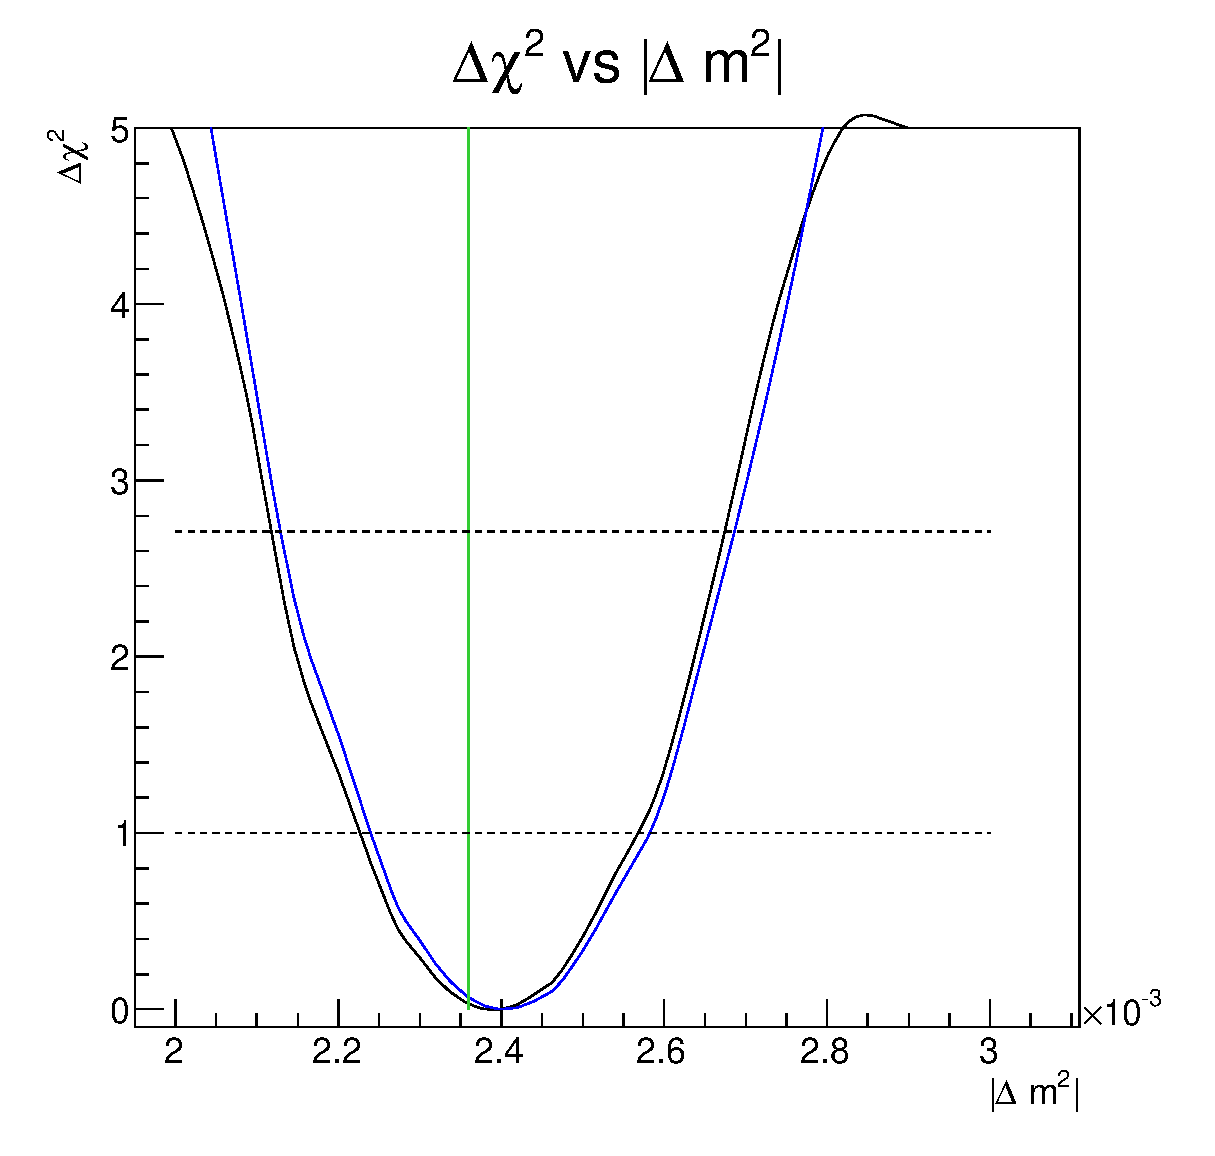
\includegraphics[width=9pc]{./images/appendix/sensitivity_studies/sensitivity_point9_chisq_vs_dm23sq.eps}
\caption {
$\Delta\chi^2$ as function of $|\Delta m^{2}|$ for true oscillation parameter point \#5.	
  $\chi^2$ was averaged over hundreds of toy-MC experiments and,
  for each experiment, it was minimized with respect to 
  $\sin^{2}\theta_{23}$, $\sin^{2}\theta_{13}$, $\delta_{CP}$
  and all relevant nuisance parameters for the joint analysis (black)
  and with respect to $\sin^{2}\theta_{23}$ and all relevant nuisance
  parameters for the disappearance analysis (blue).
  }
\label{fig:sensitivity:point5:dchisq_Dmsq}
\end{minipage}
\hspace{0.02\linewidth}
\begin{minipage}[t]{0.22\linewidth}
\center
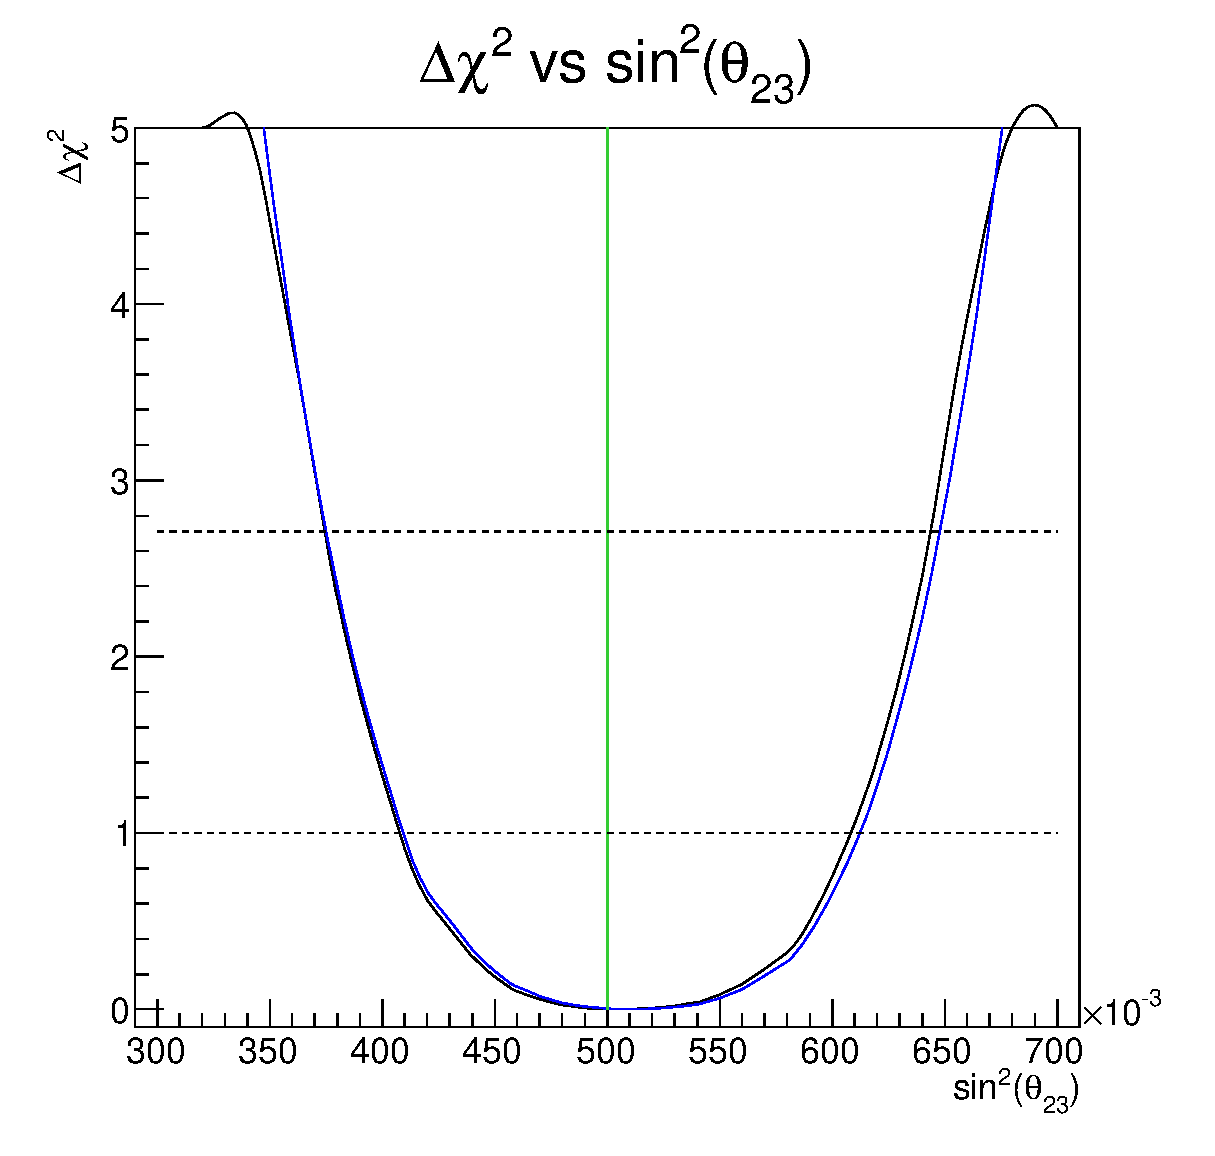
\includegraphics[width=9pc]{./images/appendix/sensitivity_studies/sensitivity_point9_chisq_vs_theta23.eps}
\caption {
  $\Delta\chi^2$ as function of $\sin^{2}\theta_{23}$ for true oscillation parameter point \#5.
  $\chi^2$ was averaged over hundreds of toy-MC experiments and,
  for each experiment, it was minimized with respect to 
  $|\Delta m^{2}|$, $\sin^{2}\theta_{13}$, $\delta_{CP}$
  and all relevant nuisance parameters for the joint analysis (black)
  and with respect to $\sin^{2}\theta_{23}$ and all relevant nuisance
  parameters for the disappearance analysis (blue).
}
\label{fig:sensitivity:point5:dchisq_sinsqtheta23}
\end{minipage}
\hspace{0.02\linewidth}
\begin{minipage}[t]{0.22\linewidth}
\center
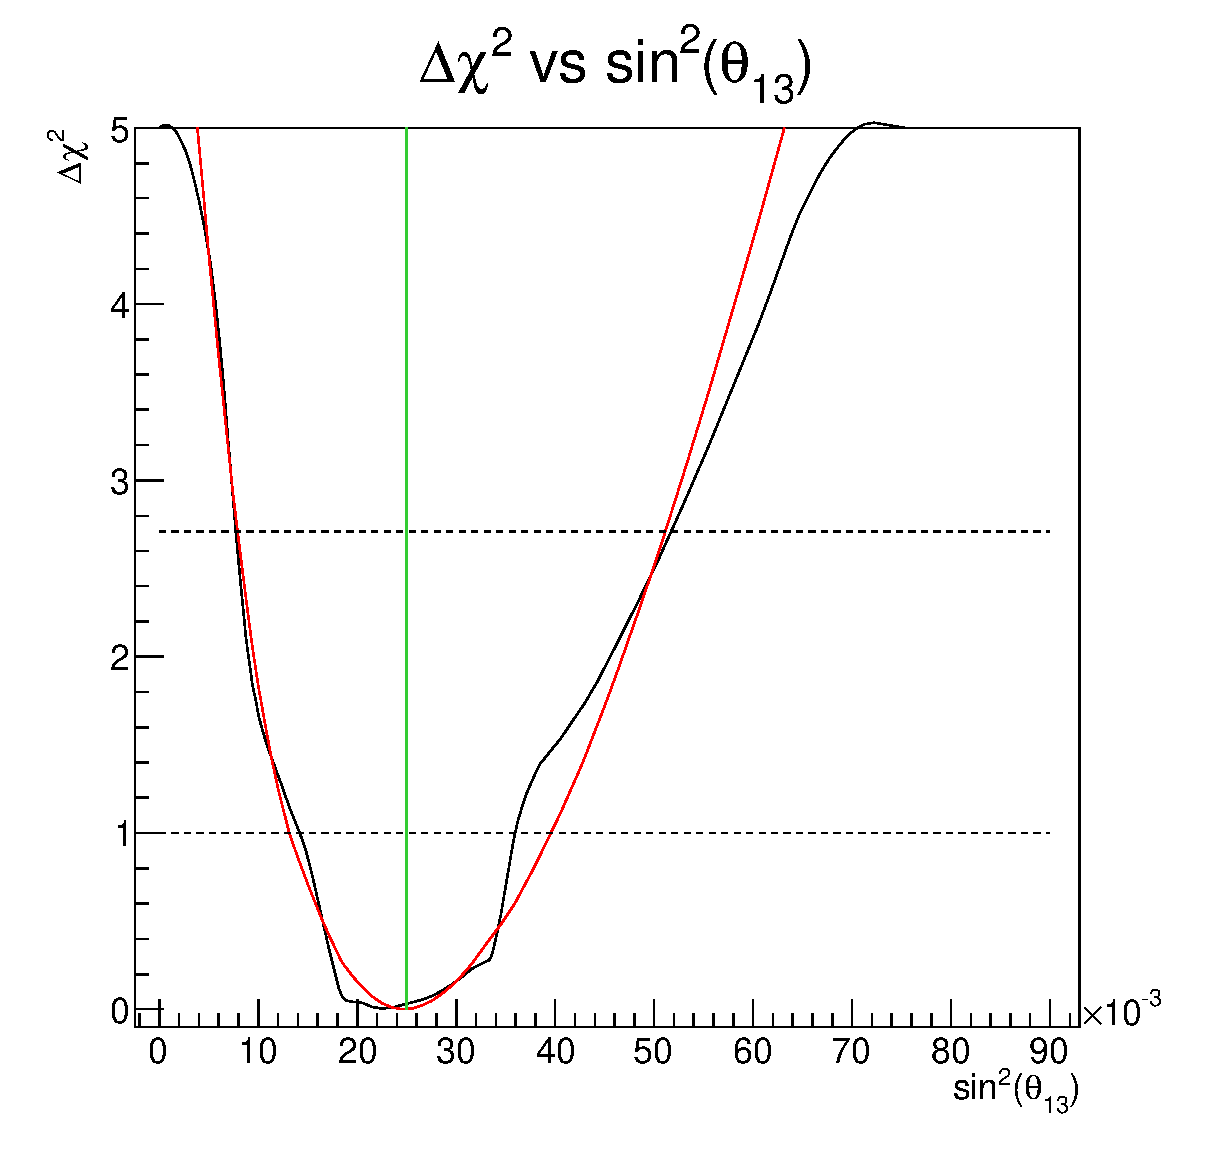
\includegraphics[width=9pc]{./images/appendix/sensitivity_studies/sensitivity_point9_chisq_vs_theta13.eps}
\caption {
  $\Delta\chi^2$ as function of $\sin^{2}\theta_{13}$ for true oscillation parameter point \#5.
  $\chi^2$ was averaged over hundreds of toy-MC experiments and,
  for each experiment, it was minimized with respect to 
  $\sin^{2}\theta_{23}$, $\sin^{2}\theta_{13}$, $\delta_{CP}$
  and all relevant nuisance parameters for the joint analysis (black)
  and with respect to all relevant nuisance parameters 
  ($\delta_{CP}$ is fixed to 0) for the appearance analysis (red).
}
\label{fig:sensitivity:point5:dchisq_sinsqtheta13}
\end{minipage}
\hspace{0.02\linewidth}
\begin{minipage}[t]{0.22\linewidth}
\center
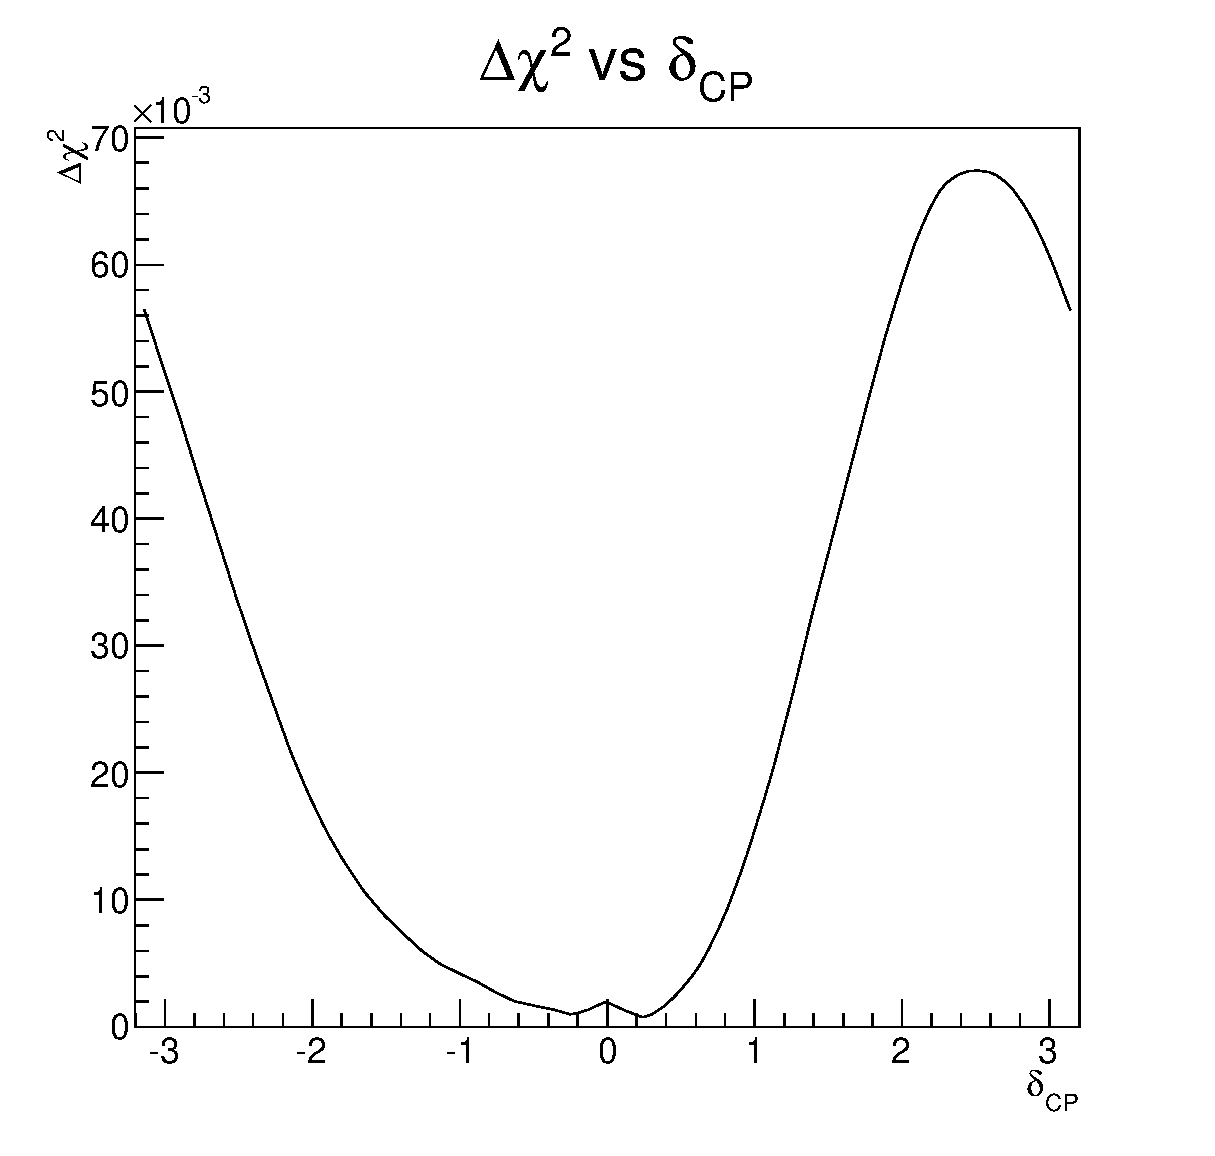
\includegraphics[width=9pc]{./images/appendix/sensitivity_studies/sensitivity_point9_chisq_vs_deltacp.eps}
\caption {
  $\Delta\chi^2$ as function of $\delta_{CP}$ for true oscillation parameter point \#5.
  $\chi^2$ was averaged over hundreds of toy-MC experiments and,
  for each experiment, it was minimized with respect to 
  $|\Delta m^{2}|$, $\sin^{2}\theta_{23}$, $\sin^{2}\theta_{13}$
  and all relevant nuisance parameters.
}
\label{fig:sensitivity:point5:dchisq_deltacp}
\end{minipage}

\end{figure*}


\clearpage

%
% ..............................................................................
% delta\chisq and contours - data
%

\begin{figure*}[htb]

\begin{minipage}[t]{0.22\linewidth}
\center
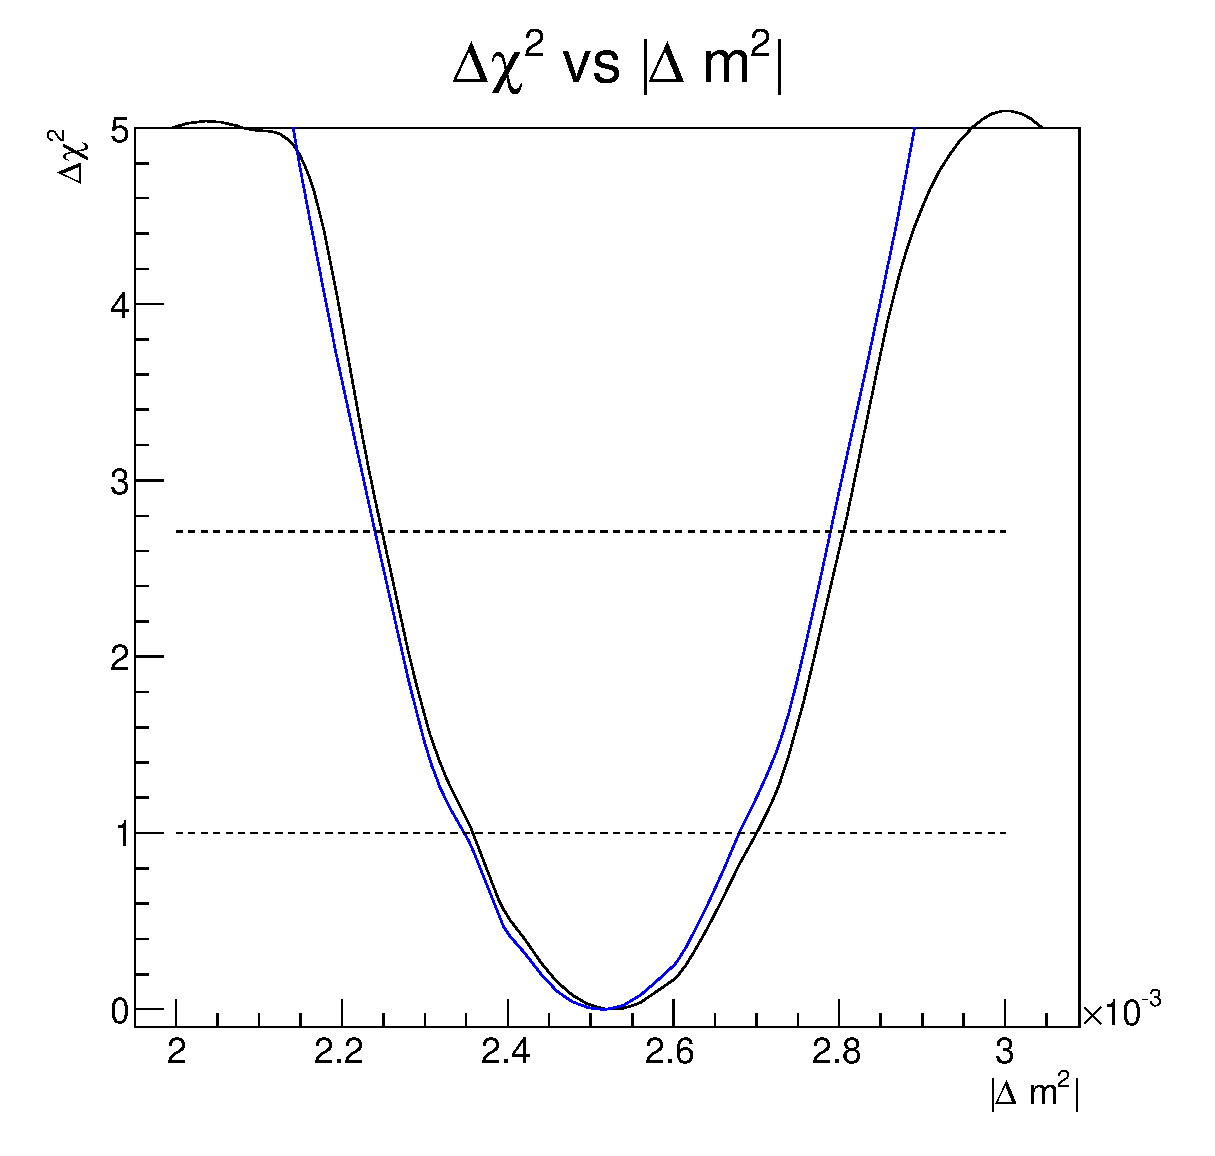
\includegraphics[width=9pc]{./images/appendix/sensitivity_studies/sensitivity_data_nh_chisq_vs_dm23sq.eps}
\caption {
  $\Delta\chi^2$ as function of $|\Delta m^{2}|$ for the best fit point found 
  for Run1+2+3 with Normal Hierarchy.
  $\chi^2$ was averaged over hundreds of toy-MC experiments and,
  for each experiment, it was minimized with respect to 
  $\sin^{2}\theta_{23}$, $\sin^{2}\theta_{13}$, $\delta_{CP}$
  and all relevant nuisance parameters for the joint analysis (black)
  and with respect to $\sin^{2}\theta_{23}$ and all relevant nuisance
  parameters for the disappearance analysis (blue).
}
\label{fig:sensitivity:data:dchisq_Dmsq}
\end{minipage}
\hspace{0.02\linewidth}
\begin{minipage}[t]{0.22\linewidth}
\center
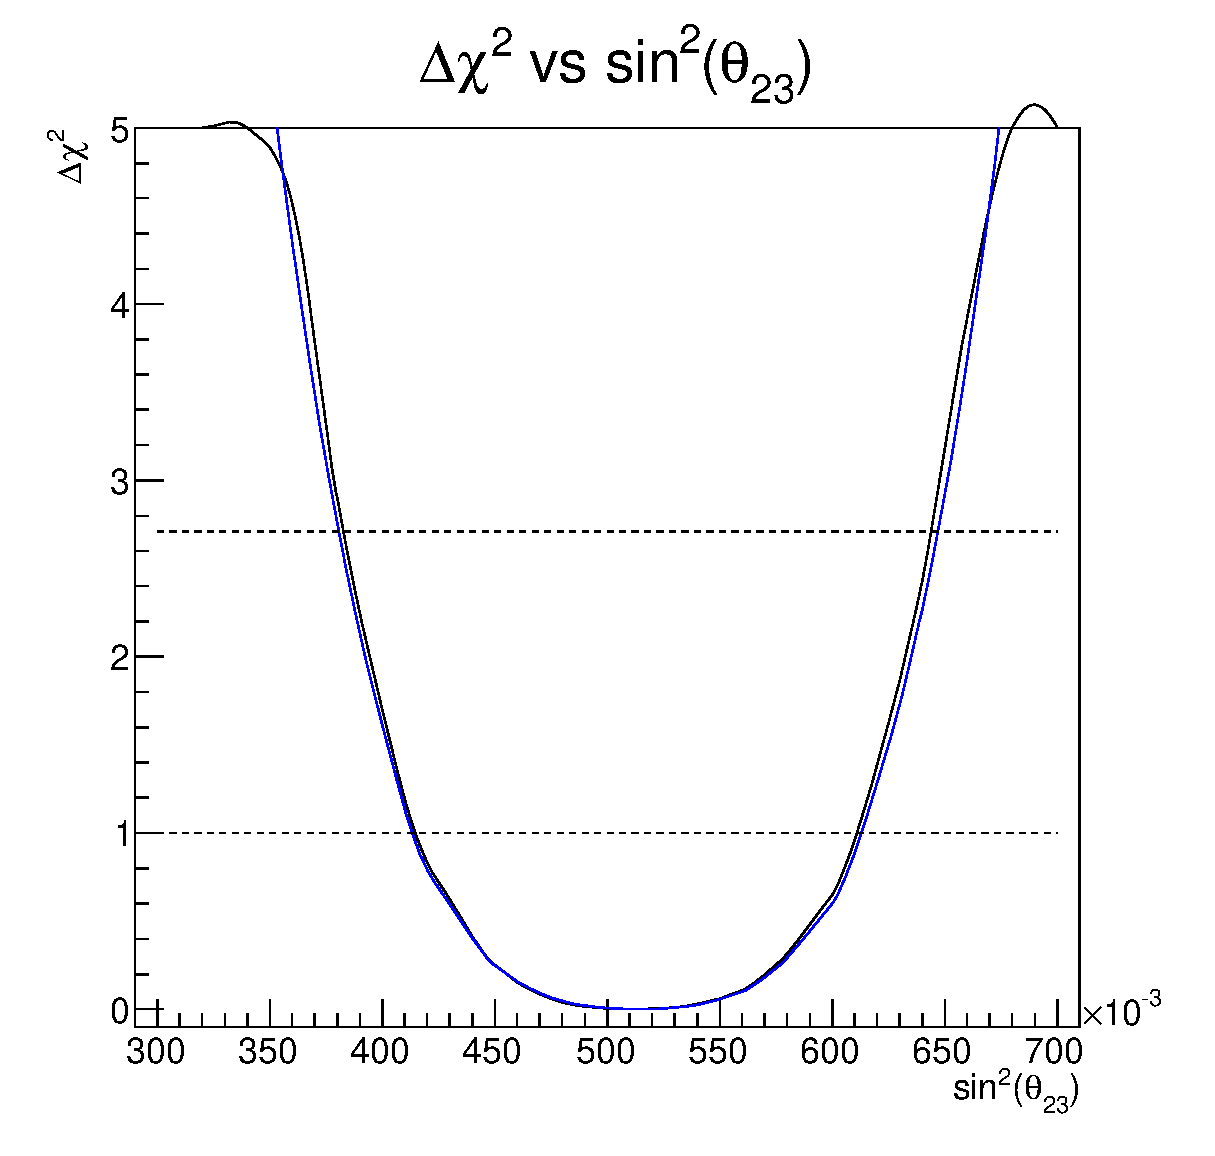
\includegraphics[width=9pc]{./images/appendix/sensitivity_studies/sensitivity_data_nh_chisq_vs_theta23.eps}
\caption {
  $\Delta\chi^2$ as function of $\sin^{2}\theta_{23}$ for the best fit point found 
  for Run1+2+3 with Normal Hierarchy.
  $\chi^2$ was averaged over hundreds of toy-MC experiments and,
  for each experiment, it was minimized with respect to 
  $\sin^{2}\theta_{23}$, $\sin^{2}\theta_{13}$, $\delta_{CP}$
  and all relevant nuisance parameters for the joint analysis (black)
  and with respect to $\sin^{2}\theta_{23}$ and all relevant nuisance
  parameters for the disappearance analysis (blue).
  }
\label{fig:sensitivity:data:dchisq_sinsqtheta23}
\end{minipage}
\hspace{0.02\linewidth}
\begin{minipage}[t]{0.22\linewidth}
\center
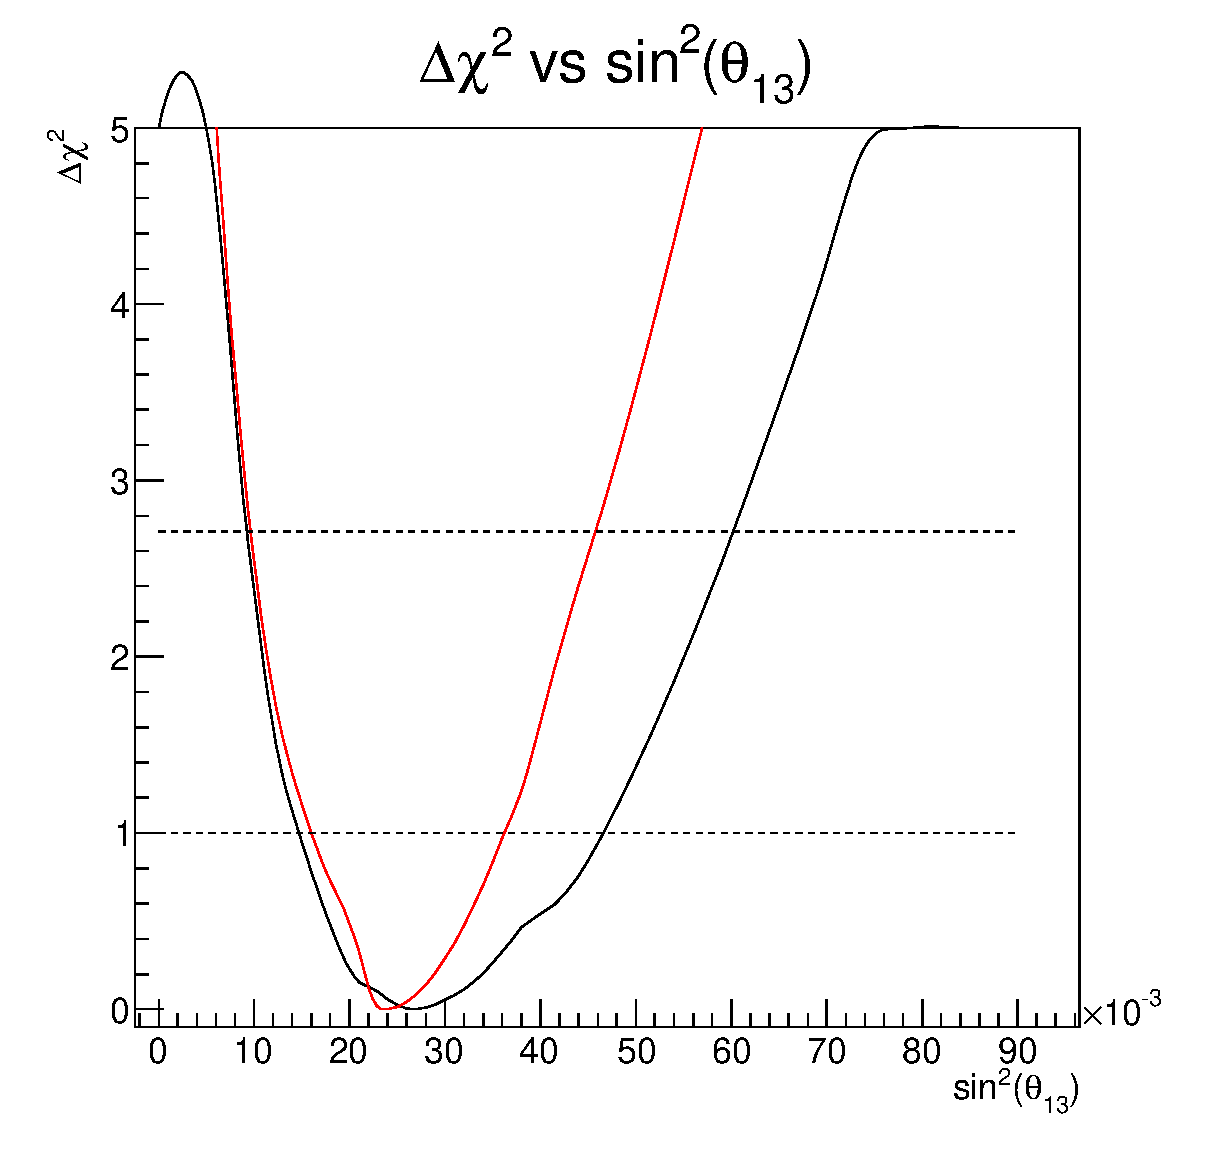
\includegraphics[width=9pc]{./images/appendix/sensitivity_studies/sensitivity_data_nh_chisq_vs_theta13.eps}
\caption {
  $\Delta\chi^2$ as function of $\sin^{2}\theta_{13}$ for the best fit point found 
  for Run1+2+3 with Normal Hierarchy.
  $\chi^2$ was averaged over hundreds of toy-MC experiments and,
  for each experiment, it was minimized with respect to 
  $\sin^{2}\theta_{23}$, $\sin^{2}\theta_{13}$, $\delta_{CP}$
  and all relevant nuisance parameters for the joint analysis (black)
  and with respect to all relevant nuisance parameters 
  ($\delta_{CP}$ is fixed to 0) for the appearance analysis (red).
  }
\label{fig:sensitivity:data:dchisq_sinsqtheta13}
\end{minipage}
\hspace{0.02\linewidth}
\begin{minipage}[t]{0.22\linewidth}
\center
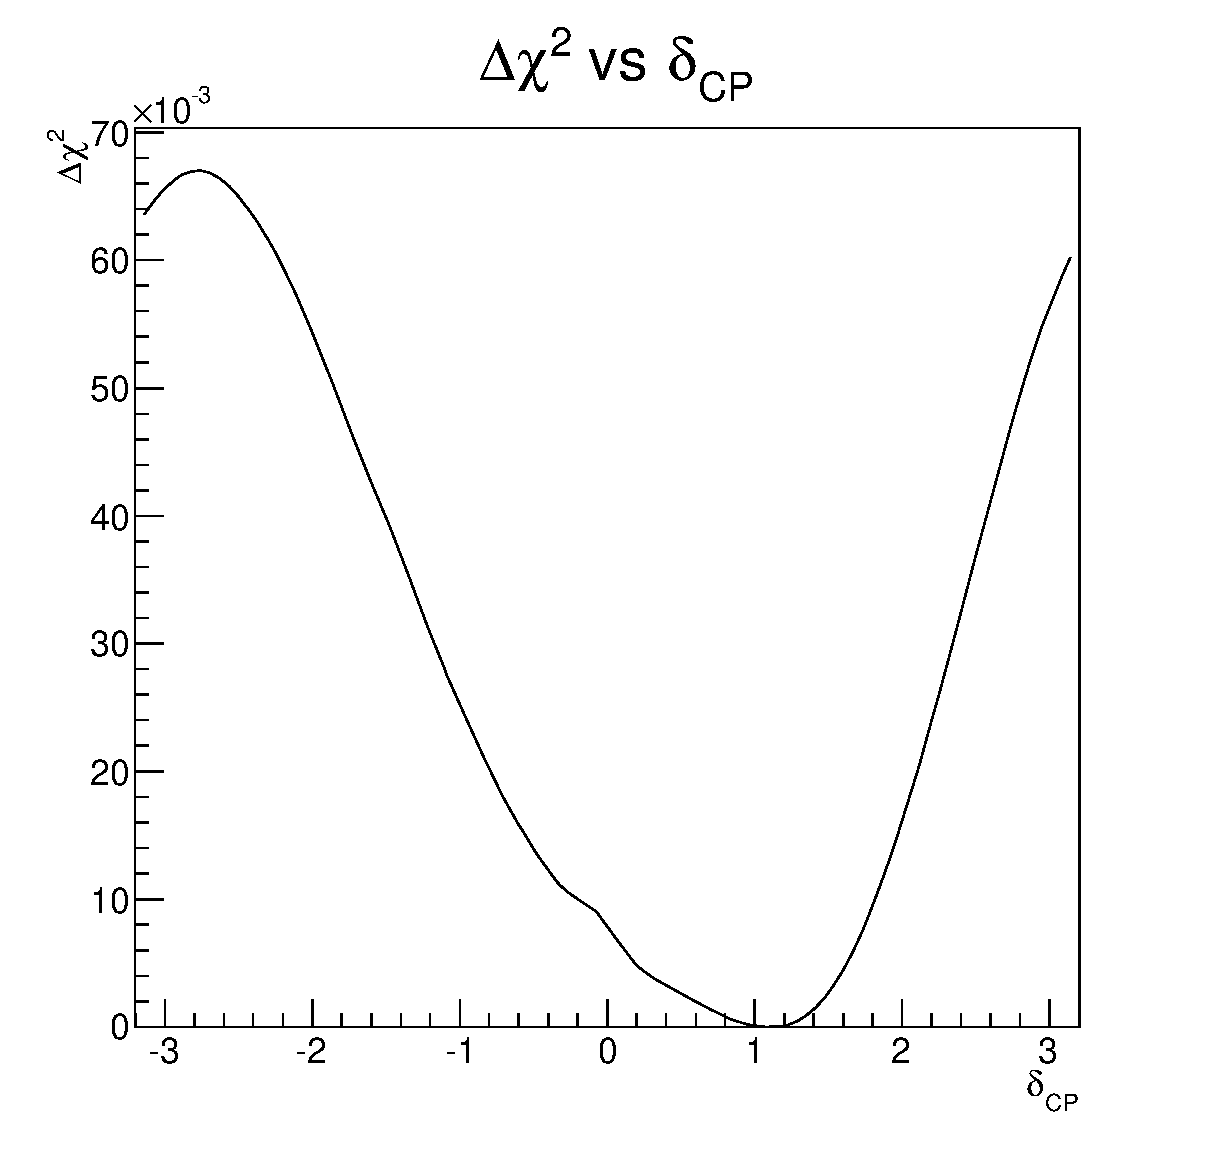
\includegraphics[width=9pc]{./images/appendix/sensitivity_studies/sensitivity_data_nh_chisq_vs_deltacp.eps}
\caption {
  $\Delta\chi^2$ as function of $\delta_{CP}$  for the best fit point found 
  for Run1+2+3 with Normal Hierarchy.
  $\chi^2$ was averaged over hundreds of toy-MC experiments and,
  for each experiment, it was minimized with respect to 
  $|\Delta m^{2}|$, $\sin^{2}\theta_{23}$, $\sin^{2}\theta_{13}$
  and all relevant nuisance parameters.
}
\label{fig:sensitivity:data:dchisq_deltacp}
\end{minipage}

\end{figure*}


\begin{figure*}[htb]

\begin{minipage}[t]{0.22\linewidth}
\center
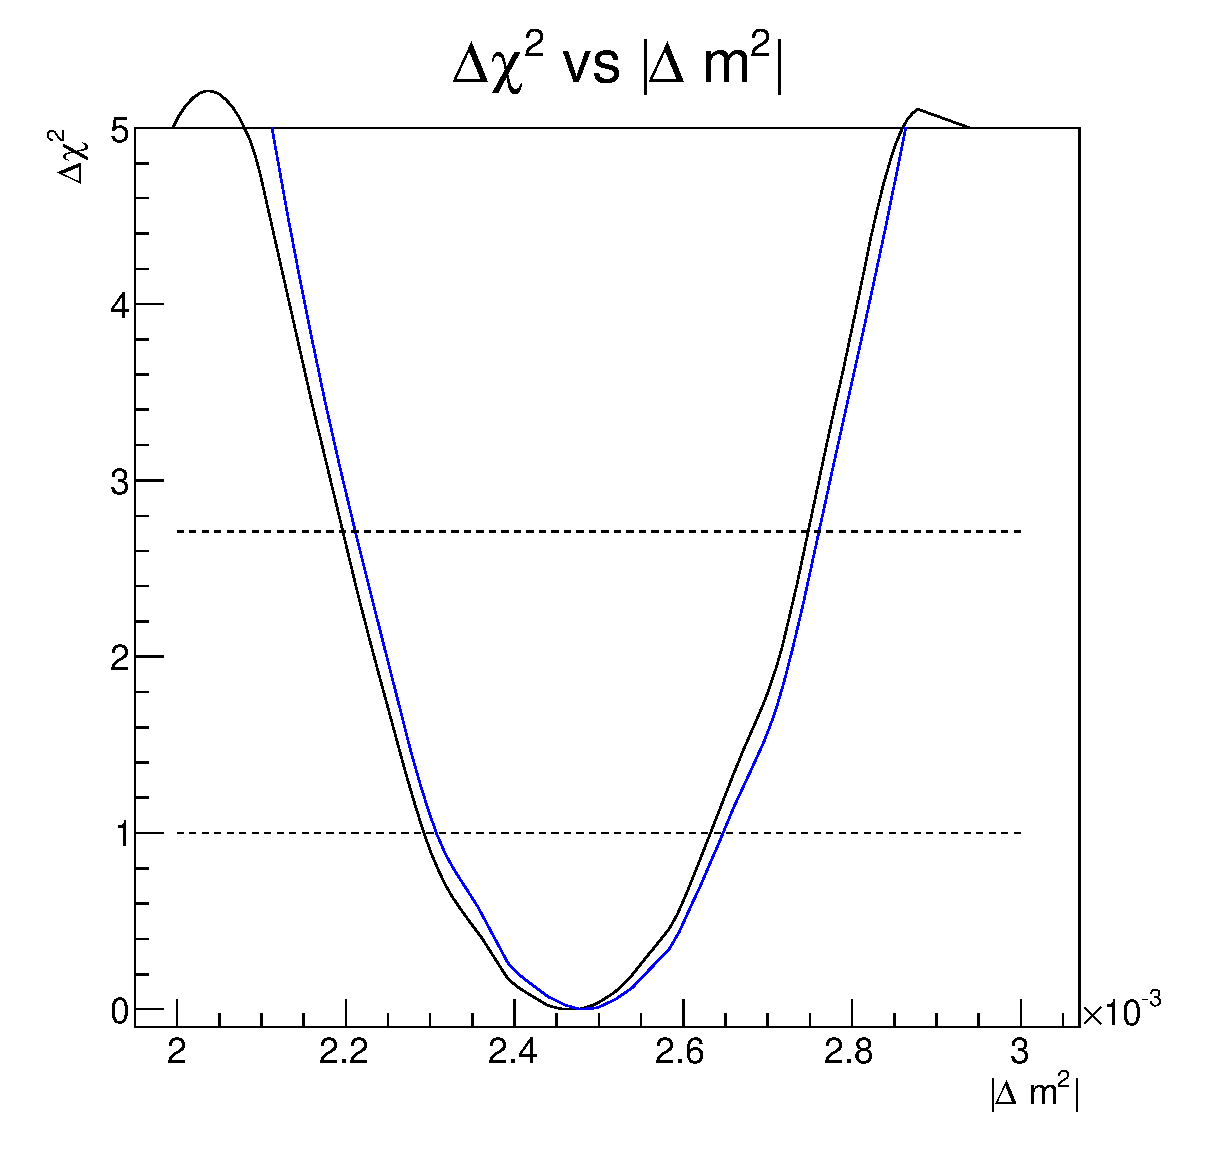
\includegraphics[width=9pc]{./images/appendix/sensitivity_studies/sensitivity_data_ih_chisq_vs_dm23sq.eps}
\caption {
  $\Delta\chi^2$ as function of $|\Delta m^{2}|$ for the best fit point found 
  for Run1+2+3 with Inverted Hierarchy.
  $\chi^2$ was averaged over hundreds of toy-MC experiments and,
  for each experiment, it was minimized with respect to 
  $\sin^{2}\theta_{23}$, $\sin^{2}\theta_{13}$, $\delta_{CP}$
  and all relevant nuisance parameters for the joint analysis (black)
  and with respect to $\sin^{2}\theta_{23}$ and all relevant nuisance
  parameters for the disappearance analysis (blue).
}
\label{fig:sensitivity:data:dchisq_Dmsq_ih}
\end{minipage}
\hspace{0.02\linewidth}
\begin{minipage}[t]{0.22\linewidth}
\center
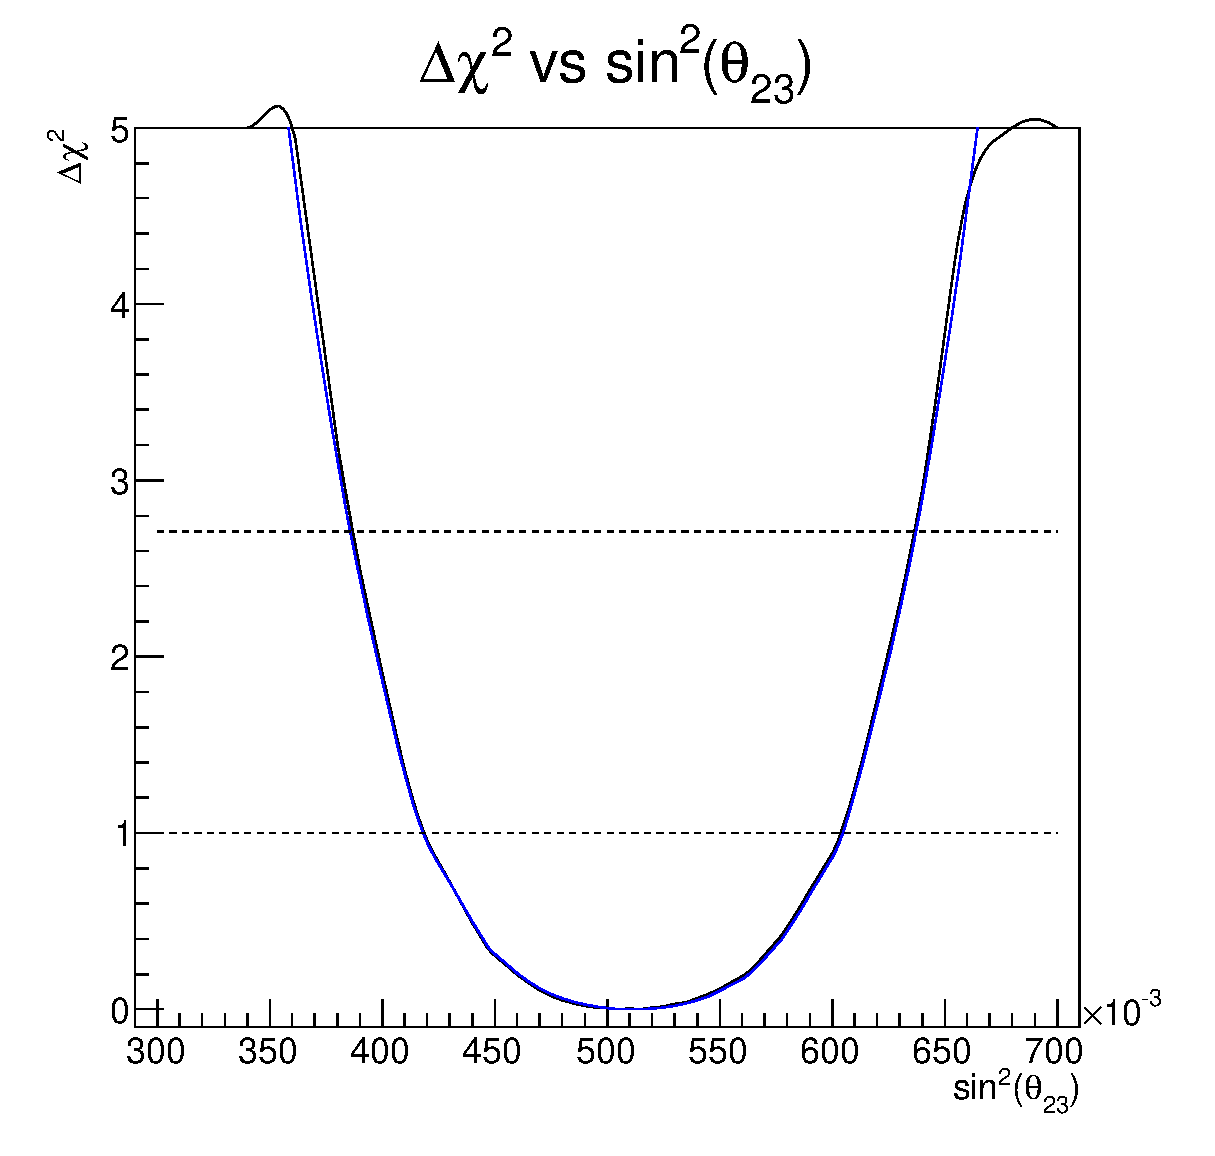
\includegraphics[width=9pc]{./images/appendix/sensitivity_studies/sensitivity_data_ih_chisq_vs_theta23.eps}
\caption {
  $\Delta\chi^2$ as function of $\sin^{2}\theta_{23}$ ffor the best fit point found 
  for Run1+2+3 with Inverted Hierarchy.
  $\chi^2$ was averaged over hundreds of toy-MC experiments and,
  for each experiment, it was minimized with respect to 
  $\sin^{2}\theta_{23}$, $\sin^{2}\theta_{13}$, $\delta_{CP}$
  and all relevant nuisance parameters for the joint analysis (black)
  and with respect to $\sin^{2}\theta_{23}$ and all relevant nuisance
  parameters for the disappearance analysis (blue).
  }
\label{fig:sensitivity:data:dchisq_sinsqtheta23_ih}
\end{minipage}
\hspace{0.02\linewidth}
\begin{minipage}[t]{0.22\linewidth}
\center
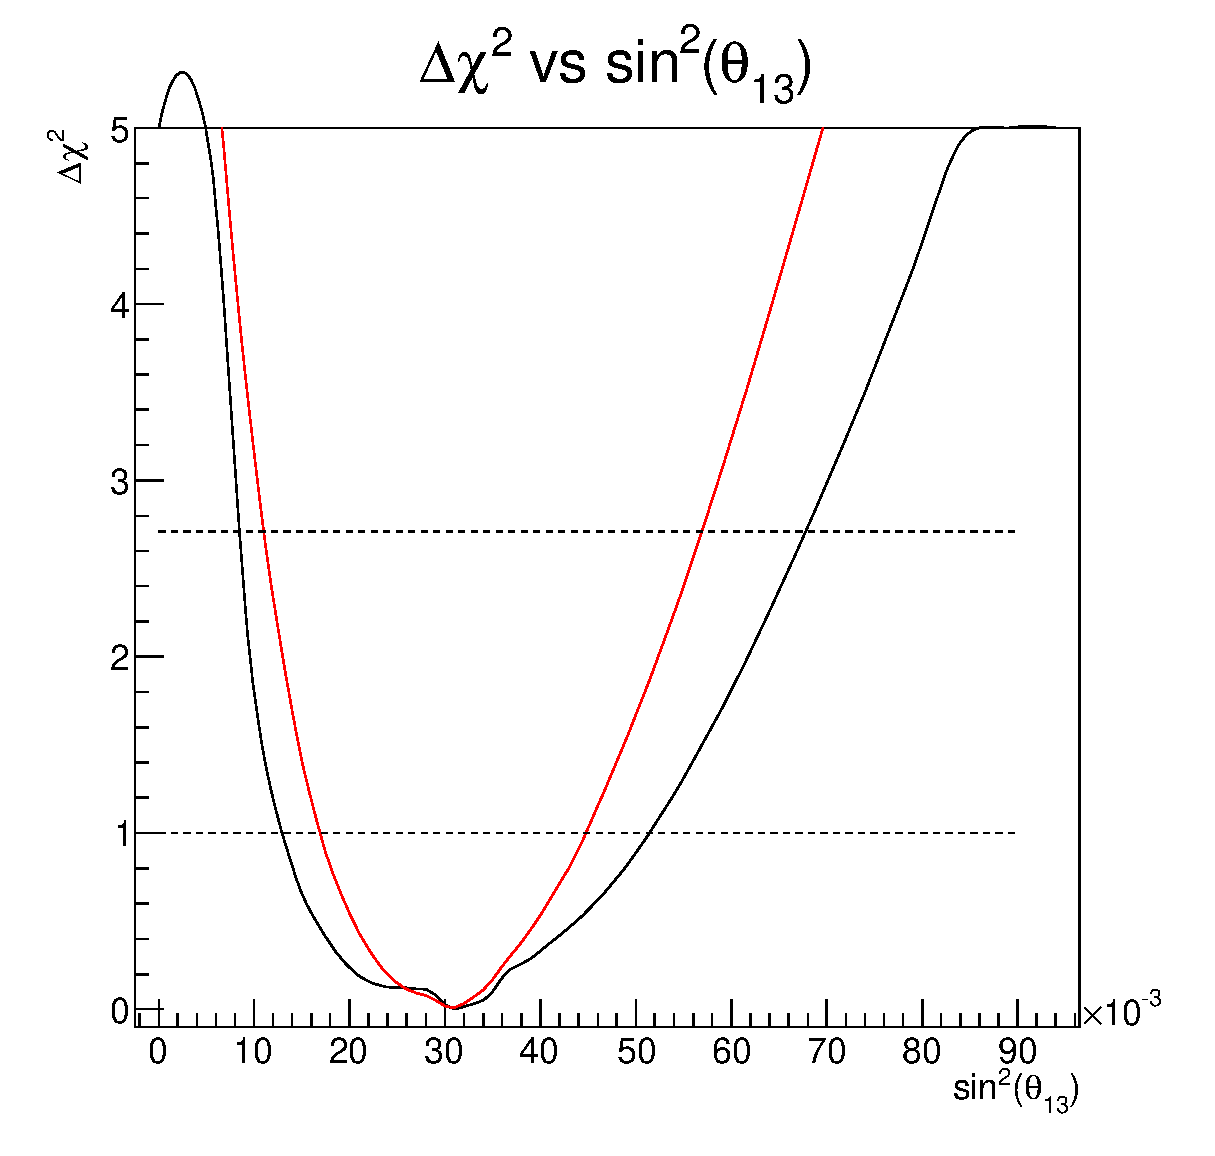
\includegraphics[width=9pc]{./images/appendix/sensitivity_studies/sensitivity_data_ih_chisq_vs_theta13.eps}
\caption {
  $\Delta\chi^2$ as function of $\sin^{2}\theta_{13}$ for the best fit point found 
  for Run1+2+3 with Inverted Hierarchy.
  $\chi^2$ was averaged over hundreds of toy-MC experiments and,
  for each experiment, it was minimized with respect to 
  $\sin^{2}\theta_{23}$, $\sin^{2}\theta_{13}$, $\delta_{CP}$
  and all relevant nuisance parameters for the joint analysis (black)
  and with respect to all relevant nuisance parameters 
  ($\delta_{CP}$ is fixed to 0) for the appearance analysis (red).
  }
\label{fig:sensitivity:data:dchisq_sinsqtheta13_ih}
\end{minipage}
\hspace{0.02\linewidth}
\begin{minipage}[t]{0.22\linewidth}
\center
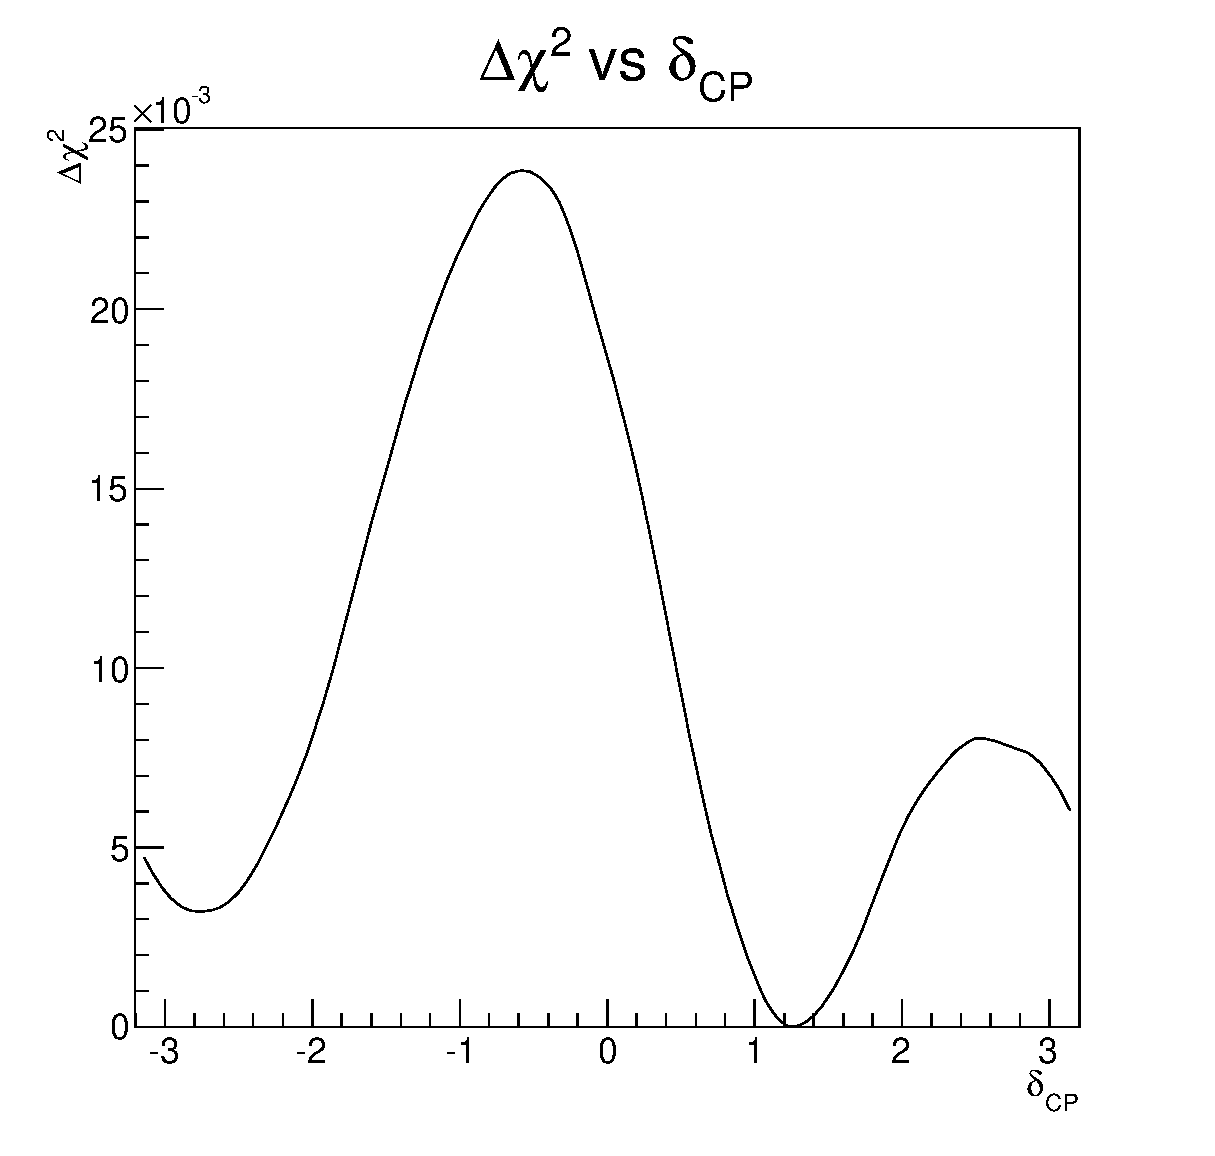
\includegraphics[width=9pc]{./images/appendix/sensitivity_studies/sensitivity_data_ih_chisq_vs_deltacp.eps}
\caption {
  $\Delta\chi^2$ as function of $\delta_{CP}$  for the best fit point found 
  for Run1+2+3 with Inverted Hierarchy.
  $\chi^2$ was averaged over hundreds of toy-MC experiments and,
  for each experiment, it was minimized with respect to 
  $|\Delta m^{2}|$, $\sin^{2}\theta_{23}$, $\sin^{2}\theta_{13}$
  and all relevant nuisance parameters.
}
\label{fig:sensitivity:data:dchisq_deltacp_ih}
\end{minipage}

\end{figure*}


\clearpage


%
% ..............................................................................
% delta\chisq and contours - data
%

\begin{figure*}[htb]

\begin{minipage}[t]{0.22\linewidth}
\center
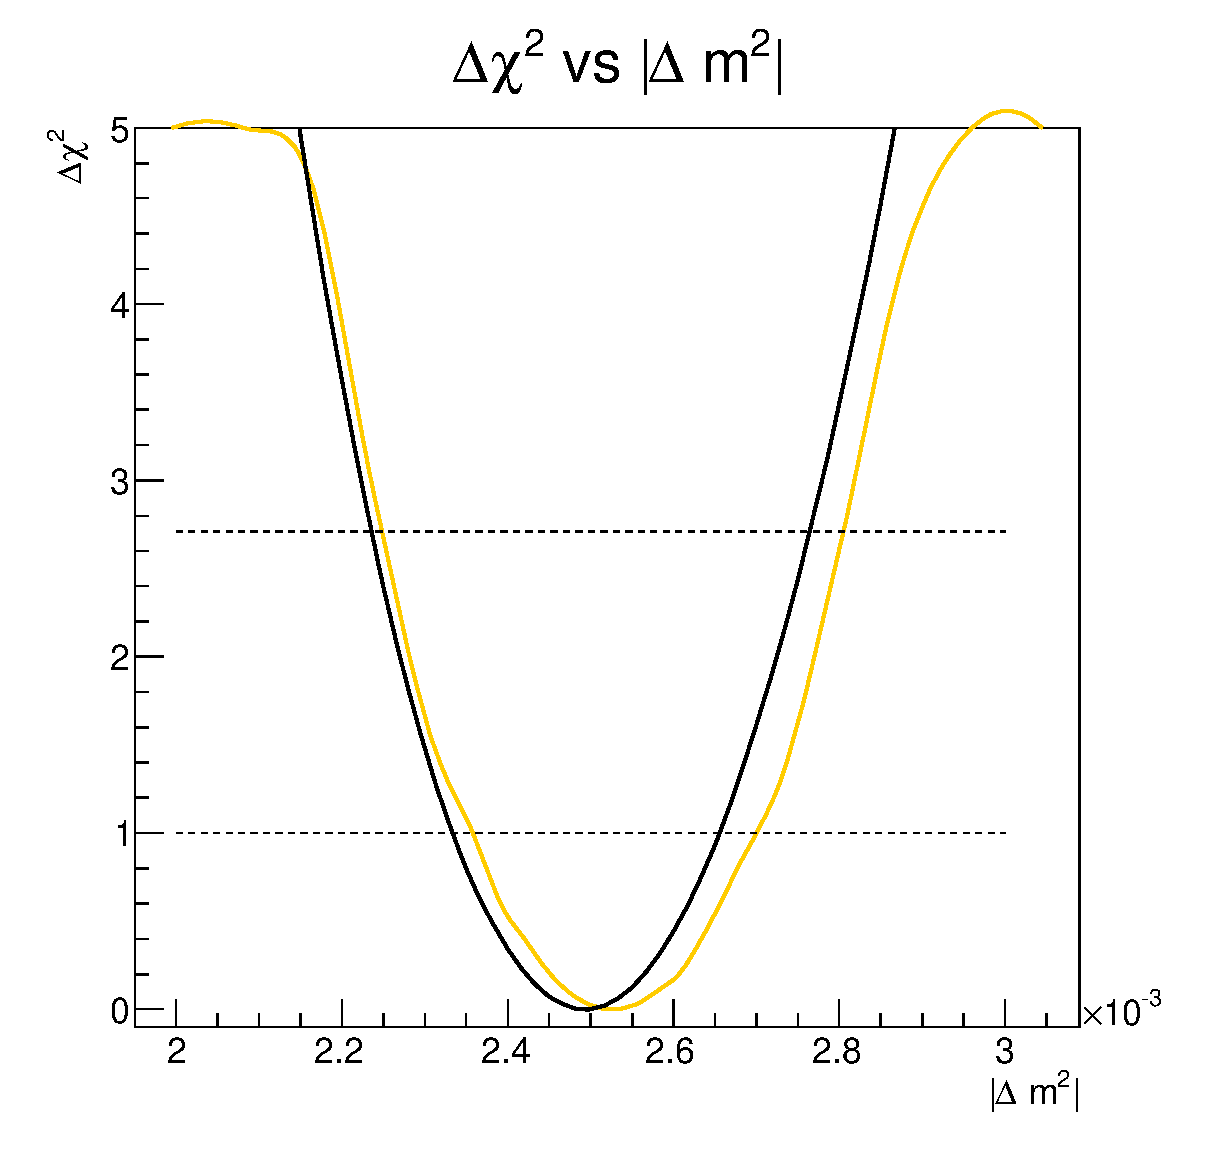
\includegraphics[width=9pc]{./images/appendix/sensitivity_studies/sensitivity_data_nh_chisq_vs_dm23sq_with_datafit.eps}
\caption {
  $\Delta\chi^2$ as function of $|\Delta m^{2}|$ for the best fit point found 
  for Run1+2+3 with Normal Hierarchy.
  Oranged line is the result of the sensitivity study, where 
  $\chi^2$ was averaged over hundreds of toy-MC experiments 
  and black line is the result of the Run1+2+3 dataset fit. 
}
\label{fig:sensitivity:data:dchisq_Dmsq_with_datafit}
\end{minipage}
\hspace{0.02\linewidth}
\begin{minipage}[t]{0.22\linewidth}
\center
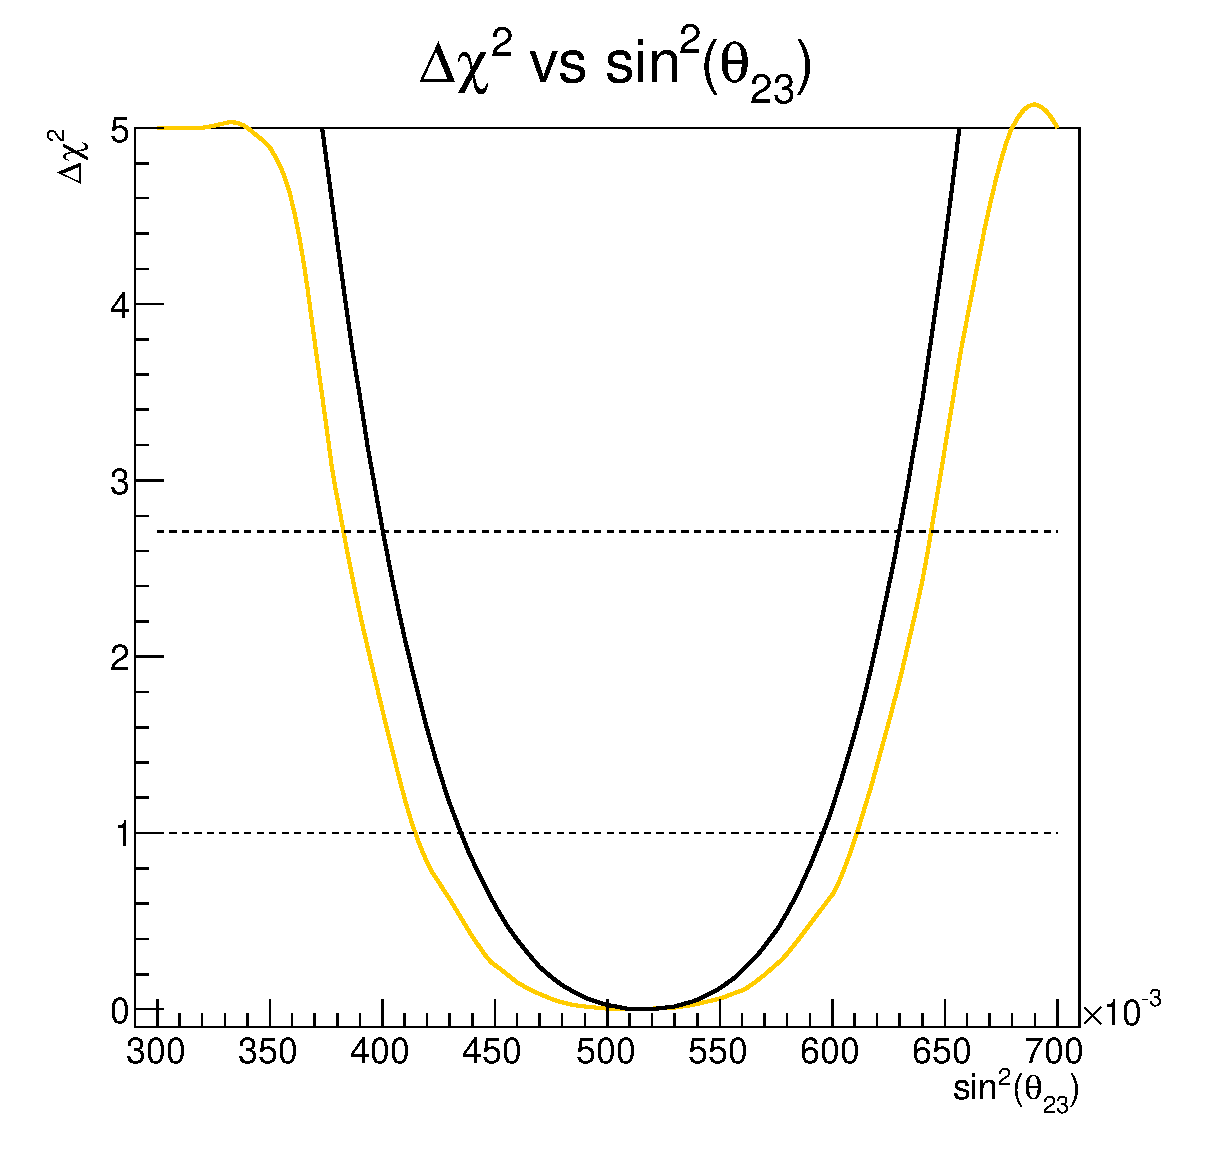
\includegraphics[width=9pc]{./images/appendix/sensitivity_studies/sensitivity_data_nh_chisq_vs_theta23_with_datafit.eps}
\caption {
  $\Delta\chi^2$ as function of $\sin^{2}\theta_{23}$ for the best fit point found 
  for Run1+2+3 with Normal Hierarchy.
 Orange line is the result of the sensitivity study, where 
  $\chi^2$ was averaged over hundreds of toy-MC experiments 
  and black line is the result of the Run1+2+3 dataset fit. 
  }
\label{fig:sensitivity:data:dchisq_sinsqtheta23_with_datafit}
\end{minipage}
\hspace{0.02\linewidth}
\begin{minipage}[t]{0.22\linewidth}
\center
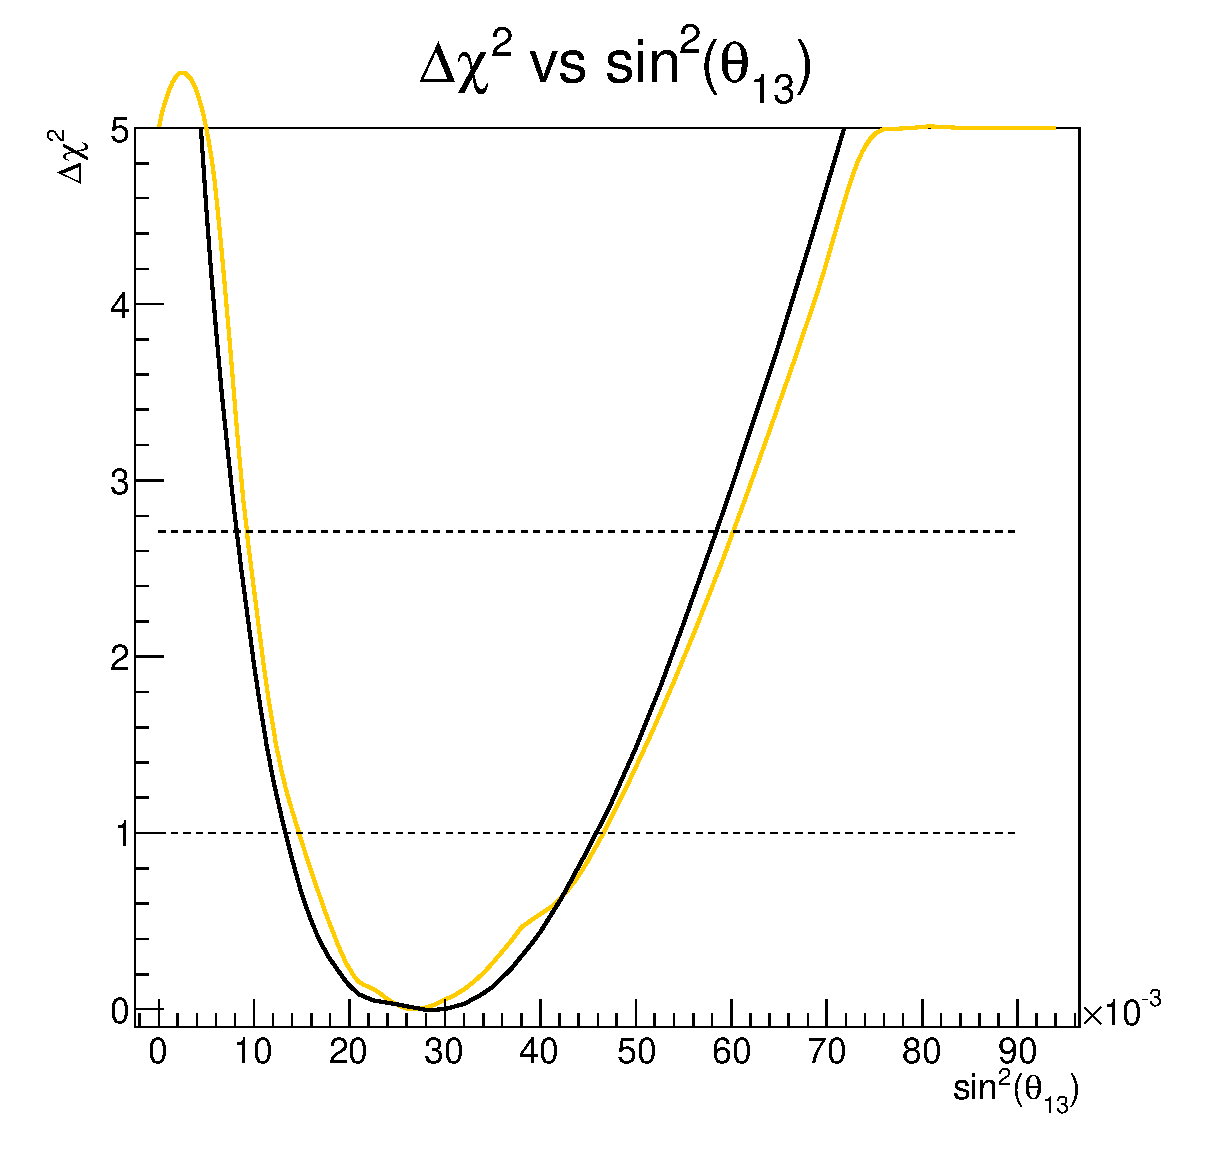
\includegraphics[width=9pc]{./images/appendix/sensitivity_studies/sensitivity_data_nh_chisq_vs_theta13_with_datafit.eps}
\caption {
  $\Delta\chi^2$ as function of $\sin^{2}\theta_{13}$ for the best fit point found 
  for Run1+2+3 with Normal Hierarchy.
 Orange line is the result of the sensitivity study, where 
  $\chi^2$ was averaged over hundreds of toy-MC experiments 
  and black line is the result of the Run1+2+3 dataset fit. 
  }
\label{fig:sensitivity:data:dchisq_sinsqtheta13_with_datafit}
\end{minipage}
\hspace{0.02\linewidth}
\begin{minipage}[t]{0.22\linewidth}
\center
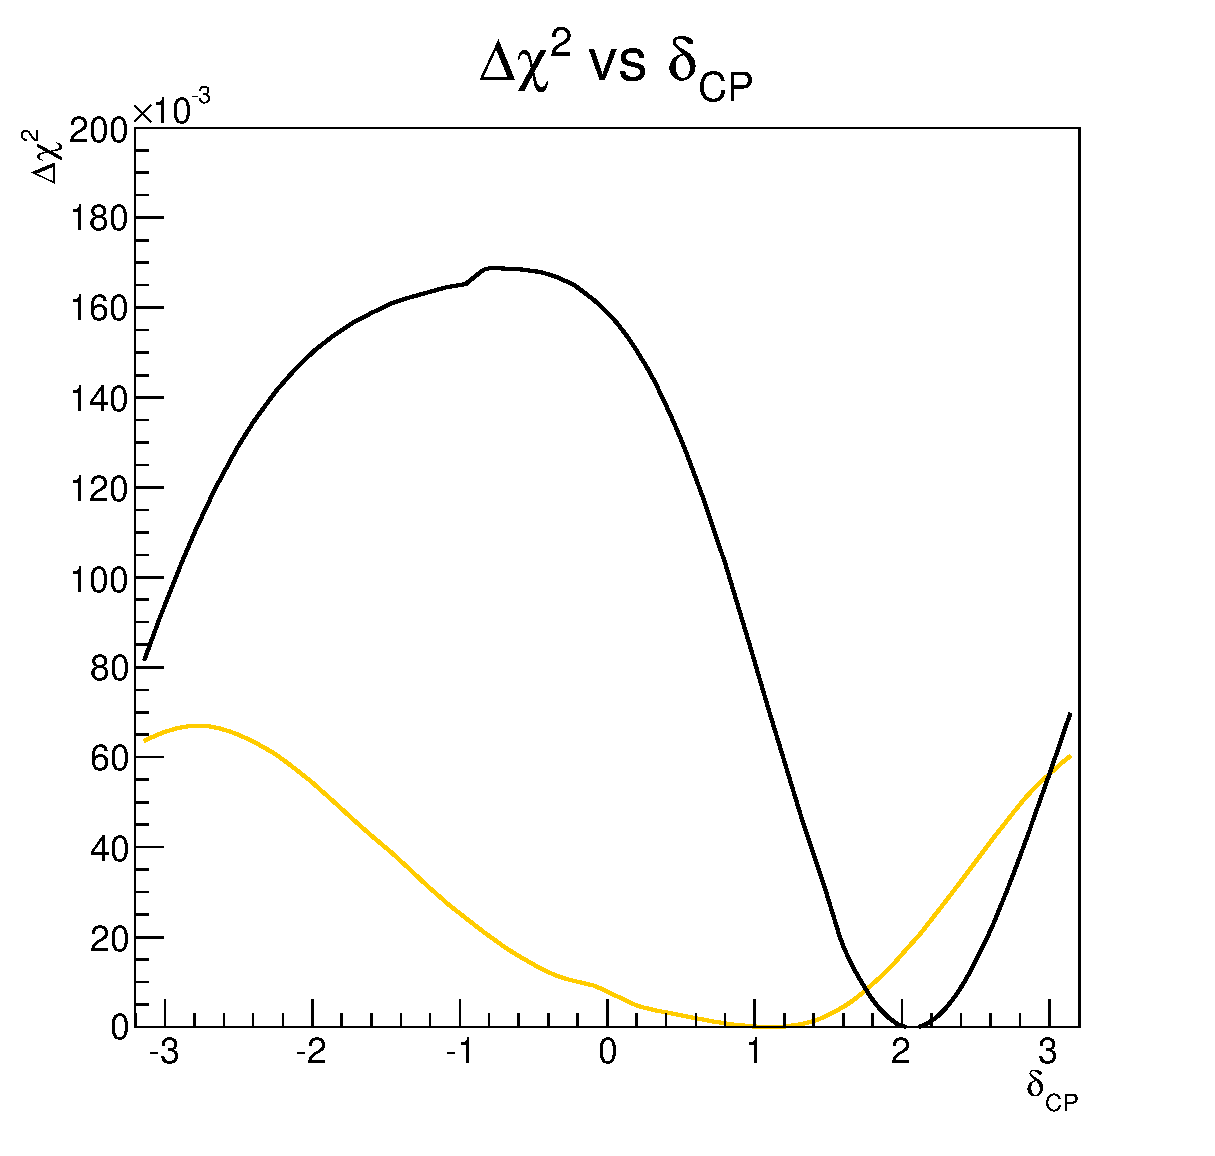
\includegraphics[width=9pc]{./images/appendix/sensitivity_studies/sensitivity_data_nh_chisq_vs_deltacp_with_datafit.eps}
\caption {
  $\Delta\chi^2$ as function of $\delta_{CP}$  for the best fit point found 
  for Run1+2+3 with Normal Hierarchy.
Orange line is the result of the sensitivity study, where 
  $\chi^2$ was averaged over hundreds of toy-MC experiments 
  and black line is the result of the Run1+2+3 dataset fit. 
}
\label{fig:sensitivity:data:dchisq_deltacp_with_datafit}
\end{minipage}

\end{figure*}



\begin{figure*}[htb]

\begin{minipage}[t]{0.22\linewidth}
\center
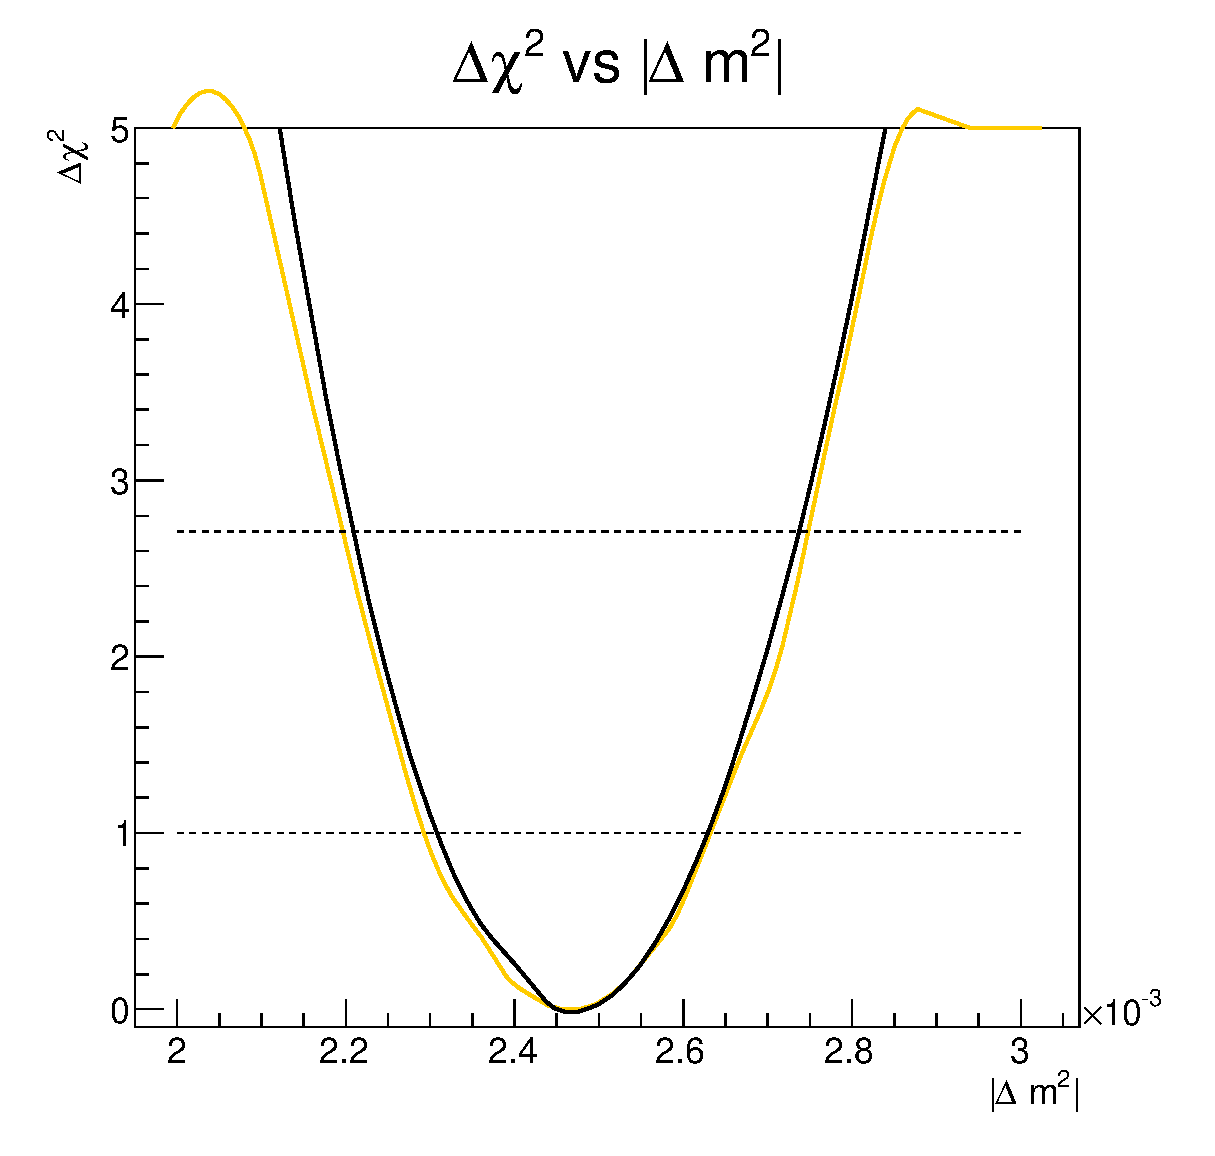
\includegraphics[width=9pc]{./images/appendix/sensitivity_studies/sensitivity_data_ih_chisq_vs_dm23sq_with_datafit.eps}
\caption {
  $\Delta\chi^2$ as function of $|\Delta m^{2}|$ for the best fit point found 
  for Run1+2+3 with Inverted Hierarchy.
  Orange line is the result of the sensitivity study, where 
  $\chi^2$ was averaged over hundreds of toy-MC experiments 
  and black line is the result of the Run1+2+3 dataset fit. 
}
\label{fig:sensitivity:data:dchisq_Dmsq_ih_with_datafit}
\end{minipage}
\hspace{0.02\linewidth}
\begin{minipage}[t]{0.22\linewidth}
\center
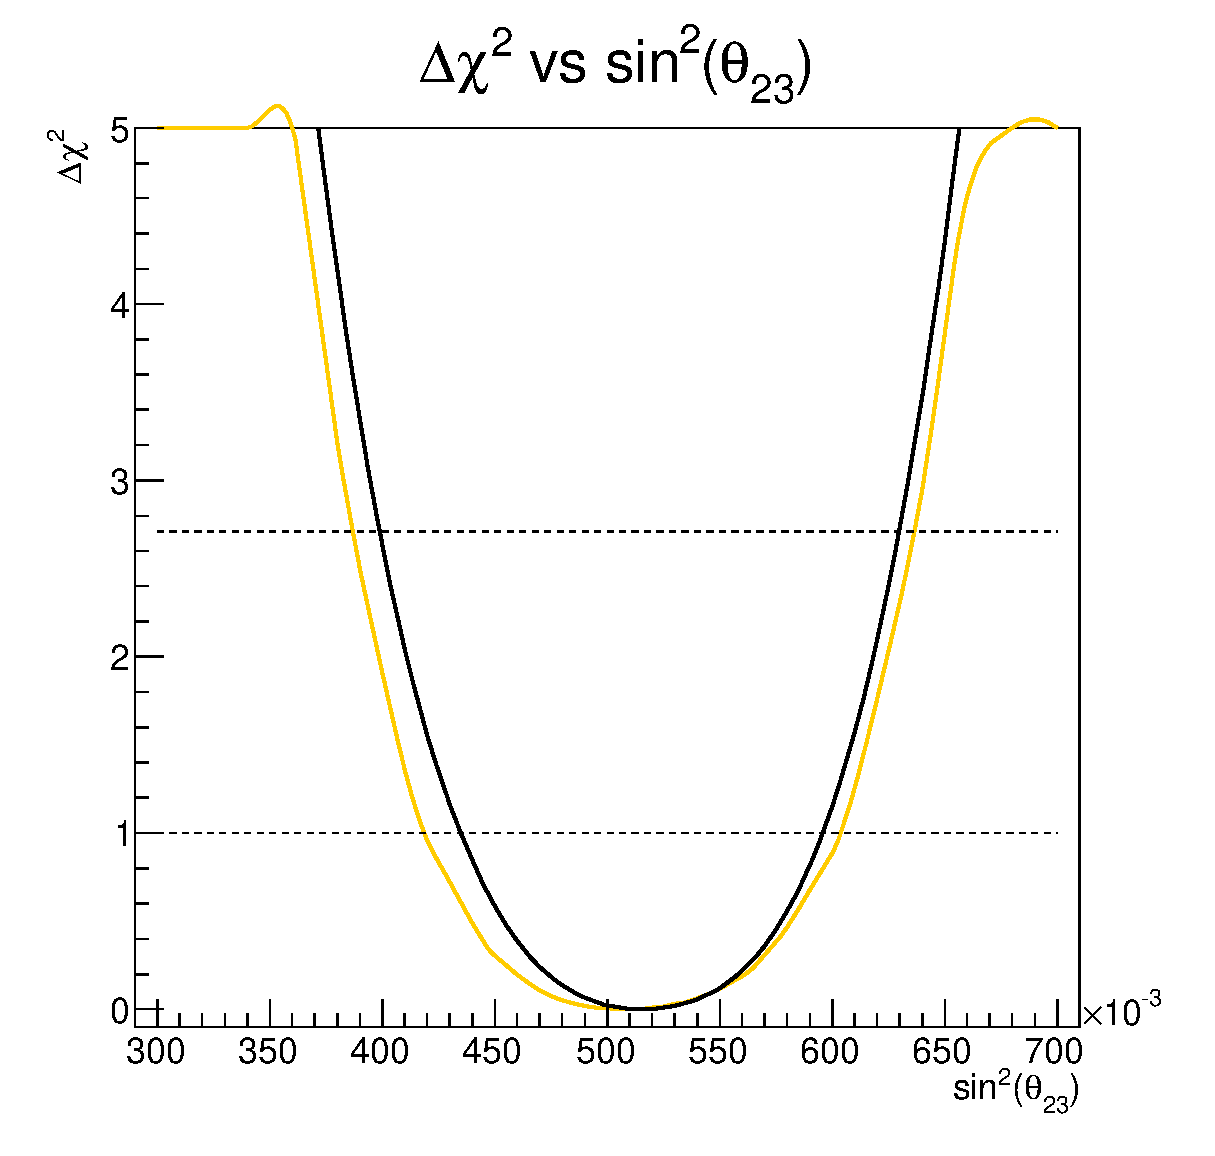
\includegraphics[width=9pc]{./images/appendix/sensitivity_studies/sensitivity_data_ih_chisq_vs_theta23_with_datafit.eps}
\caption {
  $\Delta\chi^2$ as function of $\sin^{2}\theta_{23}$ for the best fit point found 
  for Run1+2+3 with Inverted Hierarchy.
 Orange line is the result of the sensitivity study, where 
  $\chi^2$ was averaged over hundreds of toy-MC experiments 
  and black line is the result of the Run1+2+3 dataset fit. 
  }
\label{fig:sensitivity:data:dchisq_sinsqtheta23_ih_with_datafit}
\end{minipage}
\hspace{0.02\linewidth}
\begin{minipage}[t]{0.22\linewidth}
\center
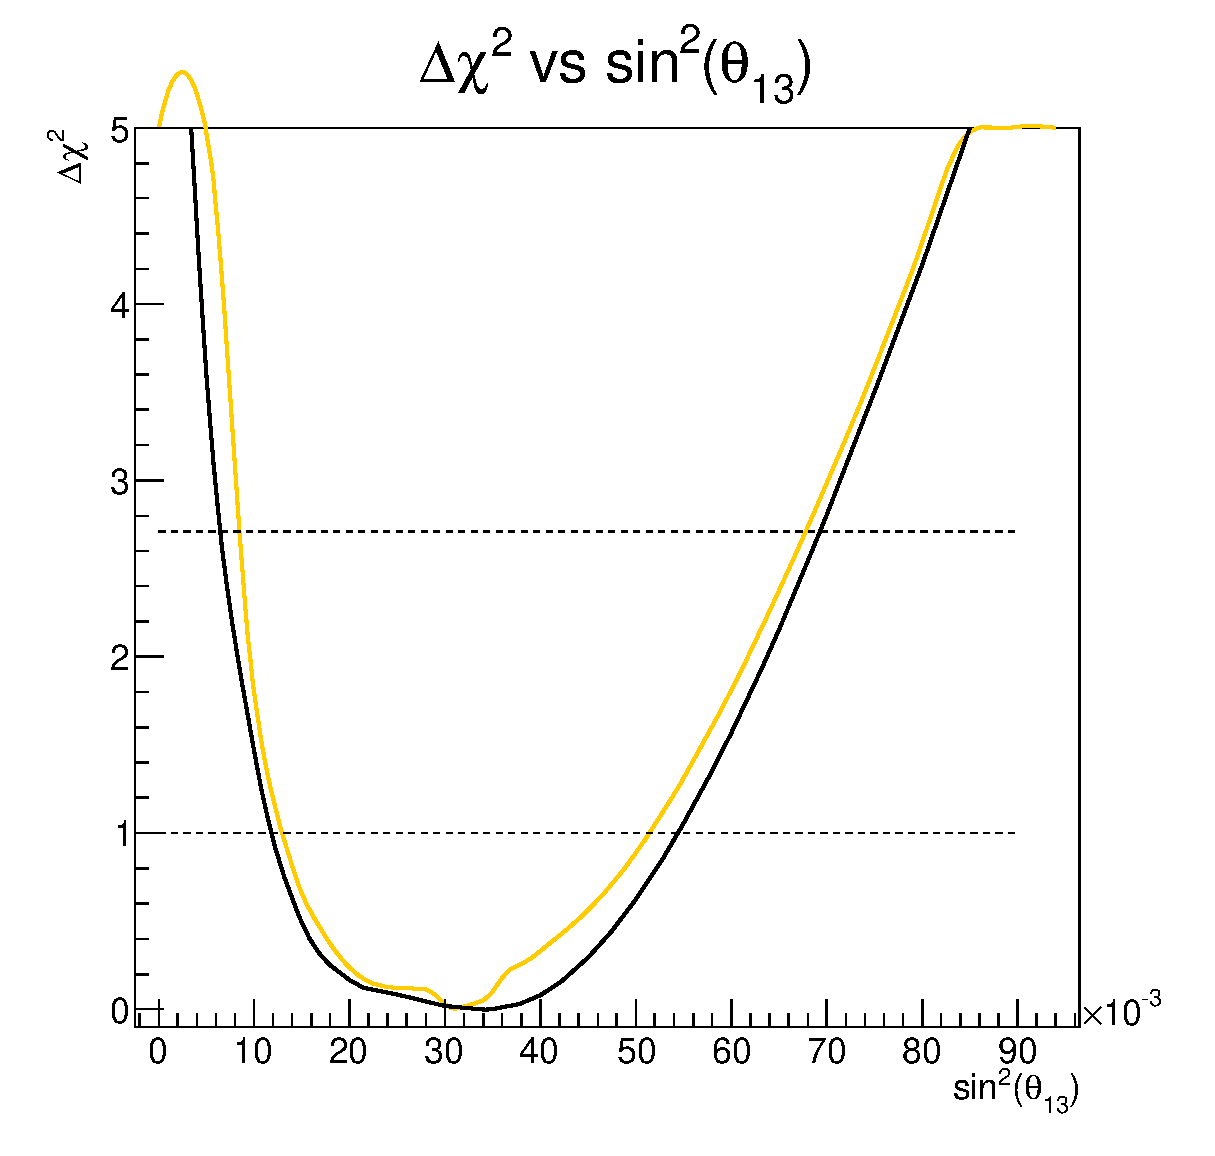
\includegraphics[width=9pc]{./images/appendix/sensitivity_studies/sensitivity_data_ih_chisq_vs_theta13_with_datafit.eps}
\caption {
  $\Delta\chi^2$ as function of $\sin^{2}\theta_{13}$ for the best fit point found 
  for Run1+2+3 with Inverted Hierarchy.
 Orange line is the result of the sensitivity study, where 
  $\chi^2$ was averaged over hundreds of toy-MC experiments 
  and black line is the result of the Run1+2+3 dataset fit. 
  }
\label{fig:sensitivity:data:dchisq_sinsqtheta13_ih_with_datafit}
\end{minipage}
\hspace{0.02\linewidth}
\begin{minipage}[t]{0.22\linewidth}
\center
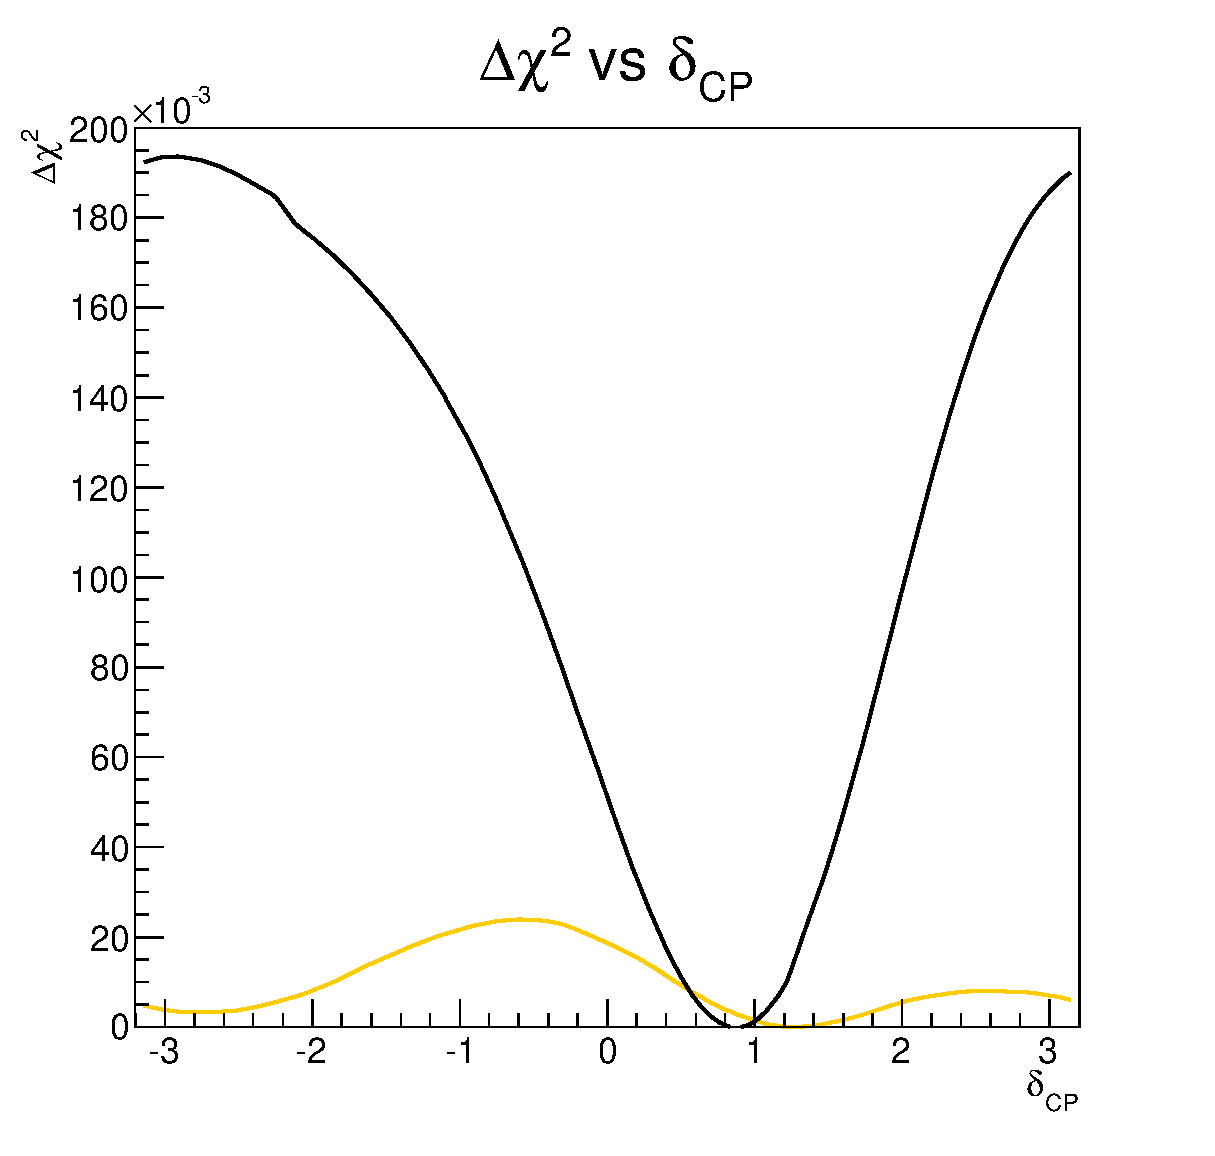
\includegraphics[width=9pc]{./images/appendix/sensitivity_studies/sensitivity_data_ih_chisq_vs_deltacp_with_datafit.eps}
\caption {
  $\Delta\chi^2$ as function of $\delta_{CP}$  for the best fit point found 
  for Run1+2+3 with Inverted Hierarchy.
Orange line is the result of the sensitivity study, where 
  $\chi^2$ was averaged over hundreds of toy-MC experiments 
  and black line is the result of the Run1+2+3 dataset fit. 
}
\label{fig:sensitivity:data:dchisq_deltacp_ih_with_datafit}
\end{minipage}

\end{figure*}



\clearpage

%
% ..............................................................................
% 2D contours - data
%

\begin{figure*}[htb]


\begin{minipage}[t]{0.48\linewidth}
\center
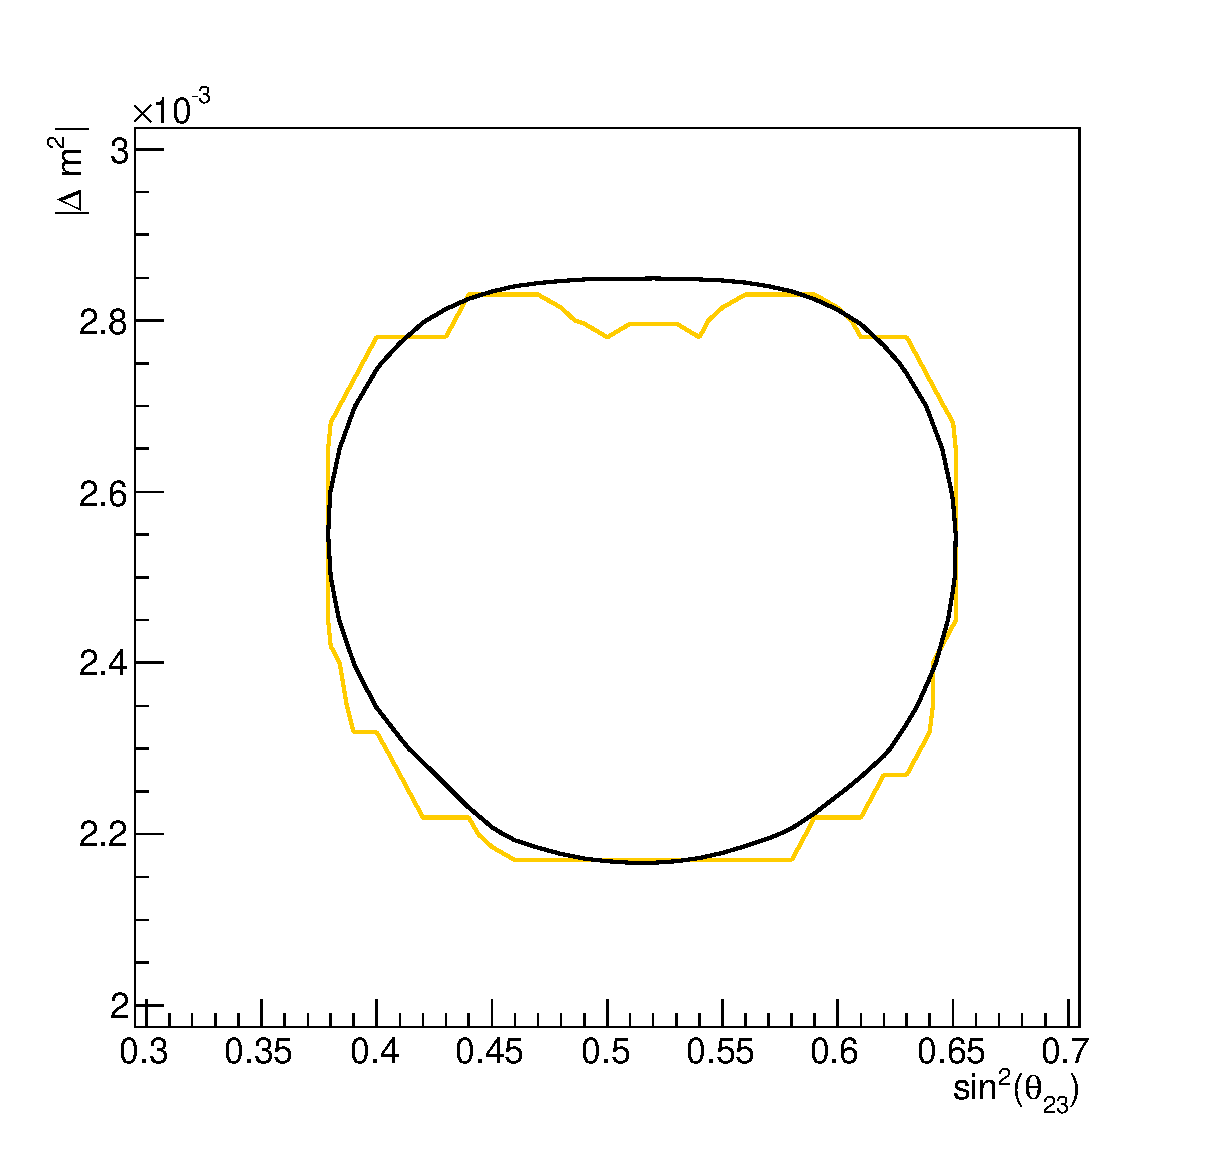
\includegraphics[width=18pc]{./images/appendix/sensitivity_studies/sensitivity_data_nh_chisq_vs_theta23_dm23sq_with_datafit.eps}
\caption {
 90\% CL region in ($\sin^{2}\theta_{23}$, $|\Delta m^{2}|$) space for the best fit point found 
  for Run1+2+3 with Normal Hierarchy.
  Orange line is the sensitivity contour that was computed by averaging
  the contours of the ensemble of hundreds of toy MC experiments and,
  for each experiment, it was minimized with respect to 
  $\sin^{2}\theta_{13}$, $\delta_{CP}$
  and all relevant nuisance parameters for the joint analysis. 
  Black line is the result of the Run1+2+3 dataset fit. 
  }
\label{fig:sensitivity:data:confreg_sinsqtheta23_Dmsq}
\end{minipage}
\hspace{0.03\linewidth}
\begin{minipage}[t]{0.48\linewidth}
\center
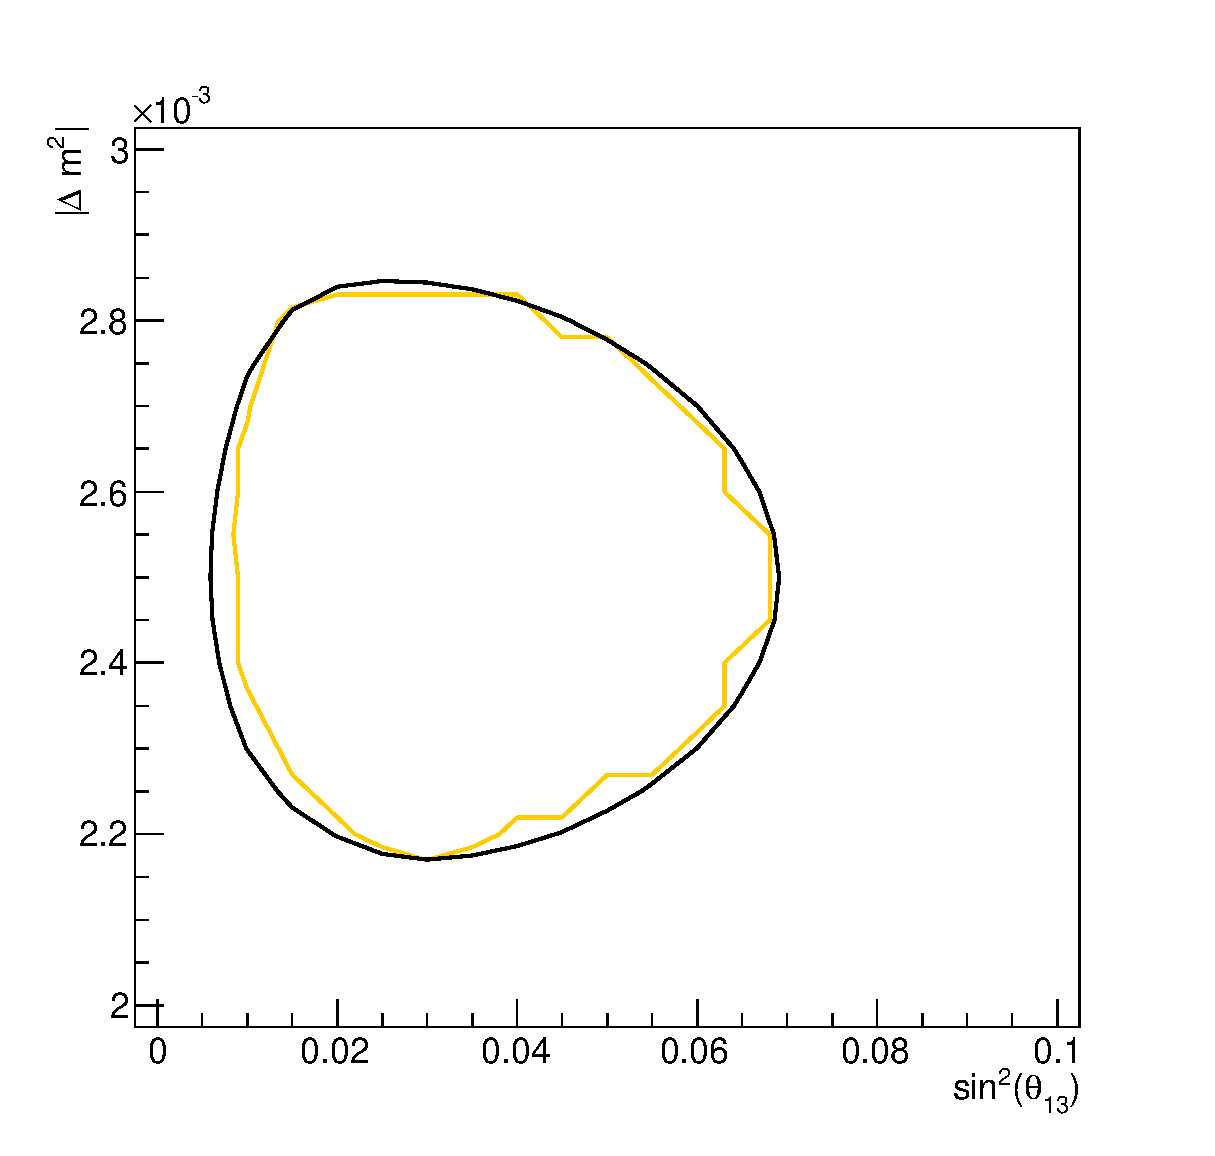
\includegraphics[width=18pc]{./images/appendix/sensitivity_studies/sensitivity_data_nh_chisq_vs_theta13_dm23sq_with_datafit.eps}
\caption {
 90\% CL region in ($\sin^{2}\theta_{13}$, $|\Delta m^{2}|$) space for the best fit point found 
  for Run1+2+3 with Normal Hierarchy.
  Orange line is the sensitivity contour that was computed by averaging
  the contours of the ensemble of hundreds of toy MC experiments and,
  for each experiment, it was minimized with respect to 
  $\sin^{2}\theta_{13}$, $\delta_{CP}$
  and all relevant nuisance parameters for the joint analysis.
  Black line is the result of the Run1+2+3 dataset fit. 
    }
\label{fig:sensitivity:data:confreg_sinsqtheta13_Dmsq}
\end{minipage}

\vfill
\vspace*{0.7cm}

\begin{minipage}[t]{0.48\linewidth}
\center
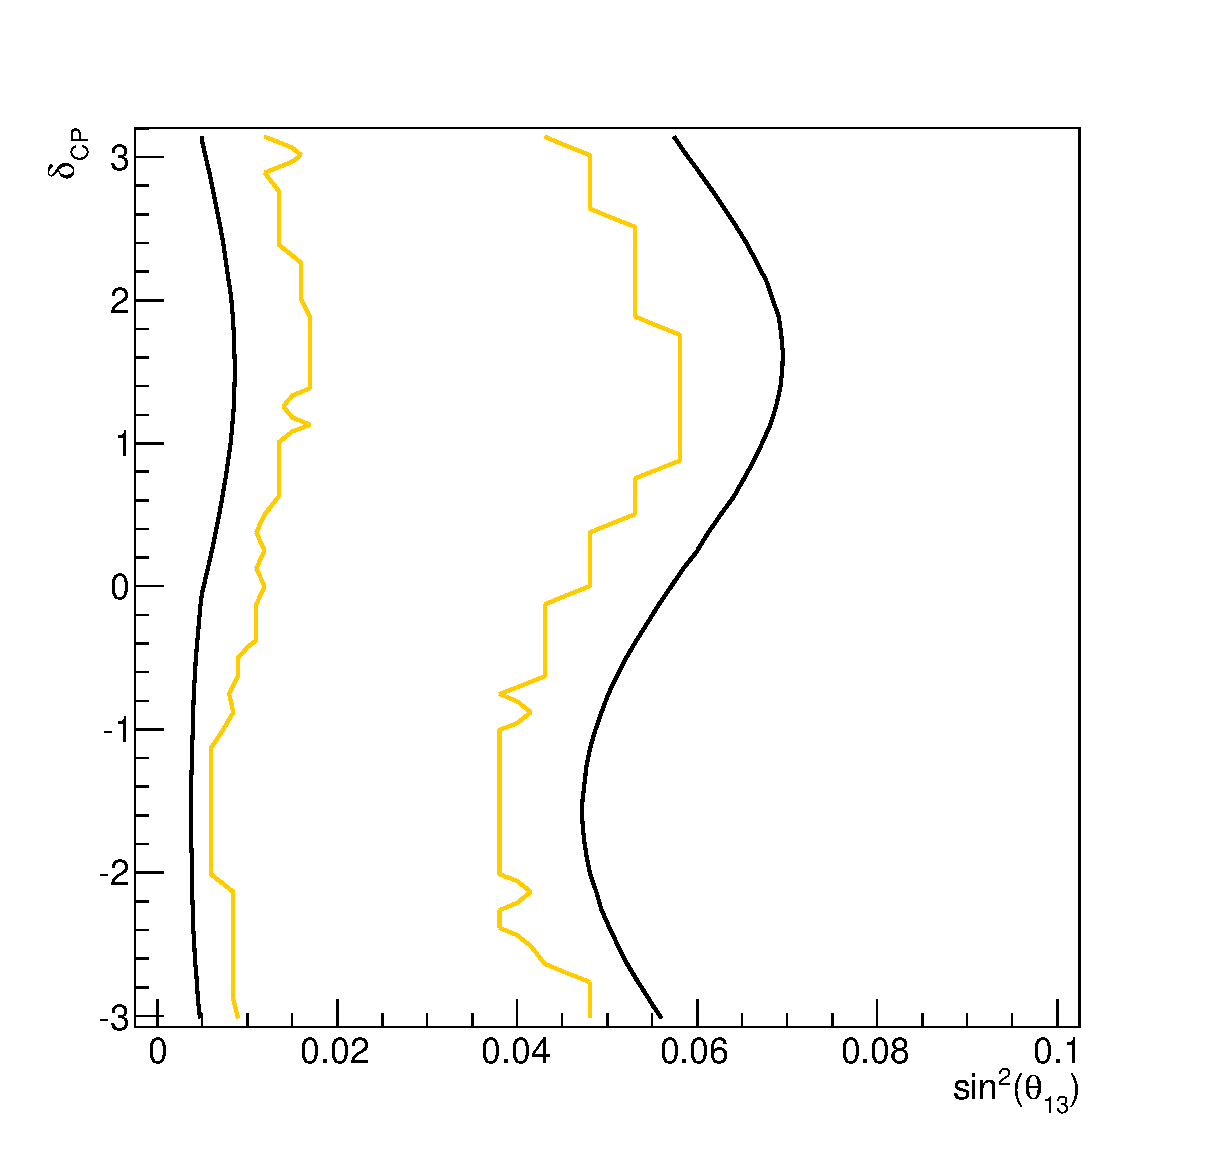
\includegraphics[width=18pc]{./images/appendix/sensitivity_studies/sensitivity_data_nh_chisq_vs_theta13_deltacp_with_datafit.eps}
\caption {
 90\% CL region in ($\sin^{2}\theta_{23}$, $\delta_{CP}$) space for the best fit point found 
  for Run1+2+3 with Normal Hierarchy.
  Orange line is the sensitivity contour that was computed by averaging
  the contours of the ensemble of hundreds of toy MC experiments and,
  for each experiment, it was minimized with respect to 
  $\sin^{2}\theta_{13}$, $\delta_{CP}$
  and all relevant nuisance parameters for the joint analysis.
  Black line is the result of the Run1+2+3 dataset fit. 
    }
\label{fig:sensitivity:data:confreg_sinsqtheta13_deltacp}
\end{minipage}
\hspace{0.03\linewidth}
\begin{minipage}[t]{0.48\linewidth}
\center
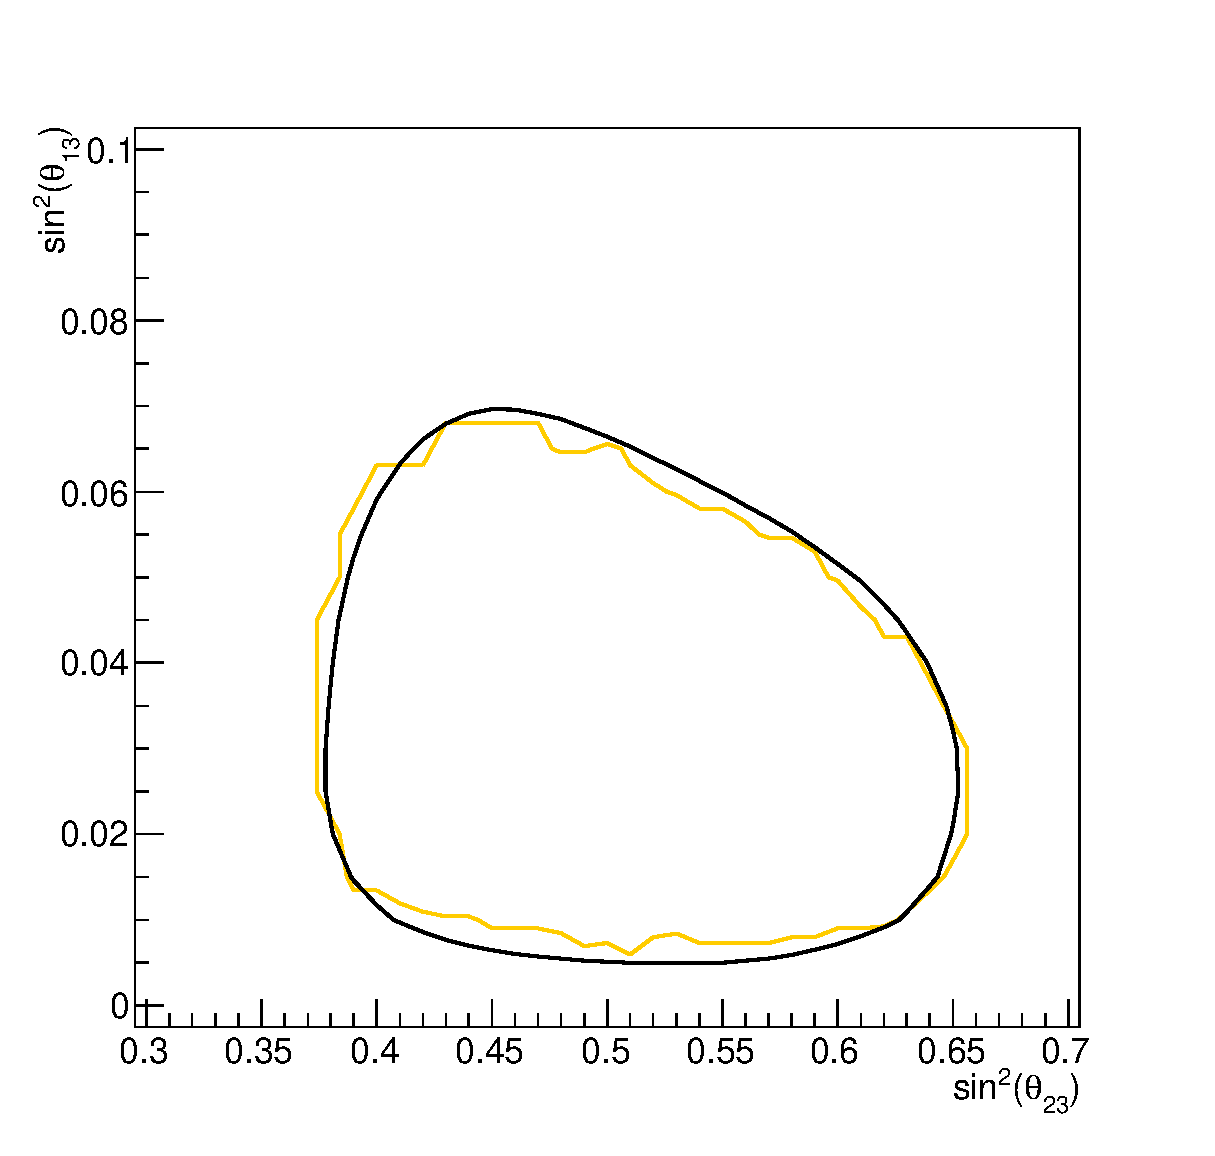
\includegraphics[width=18pc]{./images/appendix/sensitivity_studies/sensitivity_data_nh_theta13_theta23_with_datafit.eps}
\caption {
   90\% CL region in ($\sin^{2}\theta_{23}$, $\sin^{2}\theta_{13}$) space for the best fit point found 
  for Run1+2+3 with Normal Hierarchy.
  Orange line is the sensitivity contour that was computed by averaging
  the contours of the ensemble of hundreds of toy MC experiments and,
  for each experiment, it was minimized with respect to 
  $\sin^{2}\theta_{13}$, $\delta_{CP}$
  and all relevant nuisance parameters for the joint analysis.
  Black line is the result of the Run1+2+3 dataset fit. 
}
\label{fig:sensitivity:data:confreg_sinsqtheta23_sinsqtheta13}
\end{minipage}


\end{figure*}

\begin{figure*}[htb]


\begin{minipage}[t]{0.48\linewidth}
\center
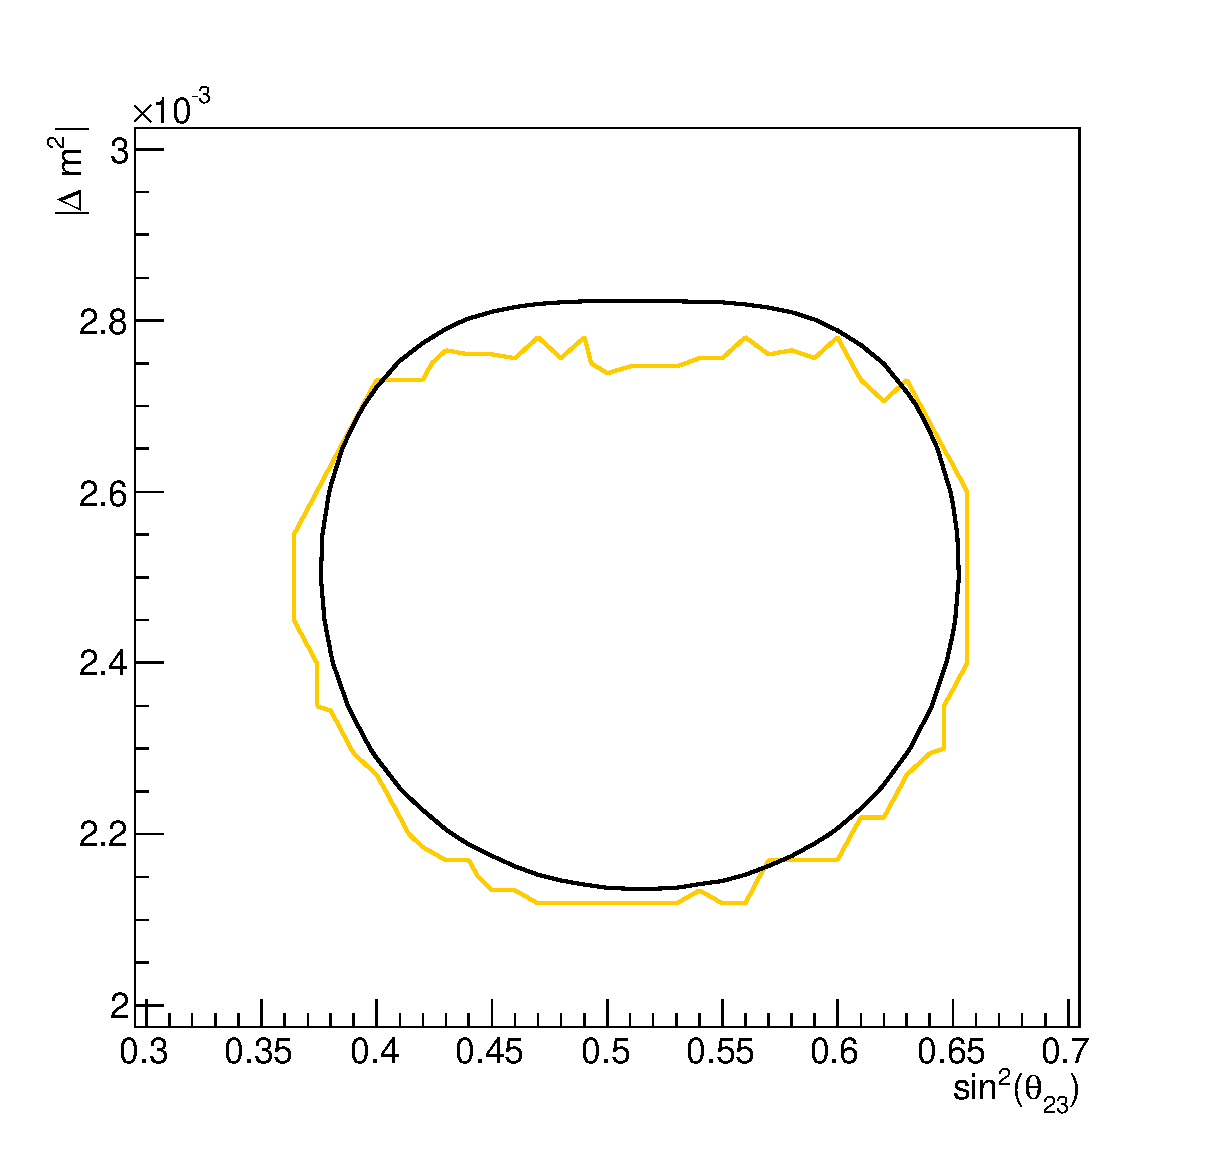
\includegraphics[width=18pc]{./images/appendix/sensitivity_studies/sensitivity_data_ih_theta23_dm23sq_with_datafit.eps}
\caption {
  90\% CL region in ($\sin^{2}\theta_{23}$, $|\Delta m^{2}|$) space for the best fit point found 
  for Run1+2+3 with Inverted Hierarchy.
  Orange line is the sensitivity contour that was computed by averaging
  the contours of the ensemble of hundreds of toy MC experiments and,
    for each experiment, it was minimized with respect to 
  $\sin^{2}\theta_{13}$, $\delta_{CP}$
  and all relevant nuisance parameters for the joint analysis.
 Black line is the result of the Run1+2+3 dataset fit. 
}
\label{fig:sensitivity:data:confreg_sinsqtheta23_Dmsq_ih}
\end{minipage}
\hspace{0.03\linewidth}
\begin{minipage}[t]{0.48\linewidth}
\center
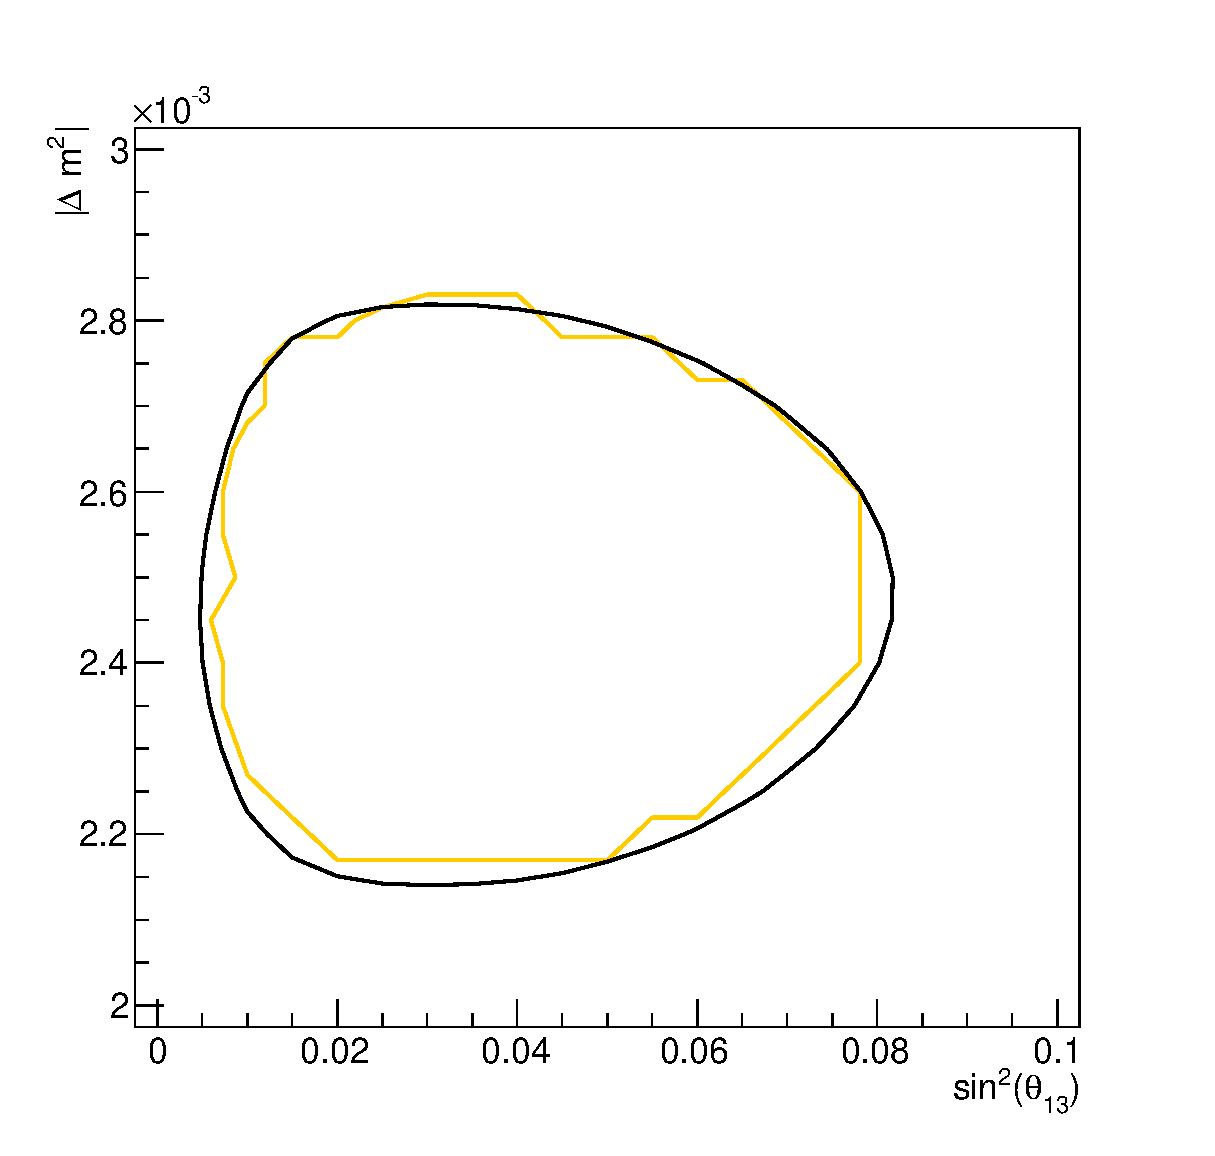
\includegraphics[width=18pc]{./images/appendix/sensitivity_studies/sensitivity_data_ih_chisq_vs_theta13_dm23sq_with_datafit.eps}
\caption {
 90\% CL region in ($\sin^{2}\theta_{13}$, $|\Delta m^{2}|$) space for the best fit point found 
  for Run1+2+3 with Inverted Hierarchy.
  Orange line is the sensitivity contour that was computed by averaging
  the contours of the ensemble of hundreds of toy MC experiments and,
  for each experiment, it was minimized with respect to 
  $\sin^{2}\theta_{13}$, $\delta_{CP}$
  and all relevant nuisance parameters for the joint analysis.
Black line is the result of the Run1+2+3 dataset fit. 
}
\label{fig:sensitivity:data:confreg_sinsqtheta13_Dmsq_ih}
\end{minipage}

\vfill
\vspace*{0.7cm}

\begin{minipage}[t]{0.48\linewidth}
\center
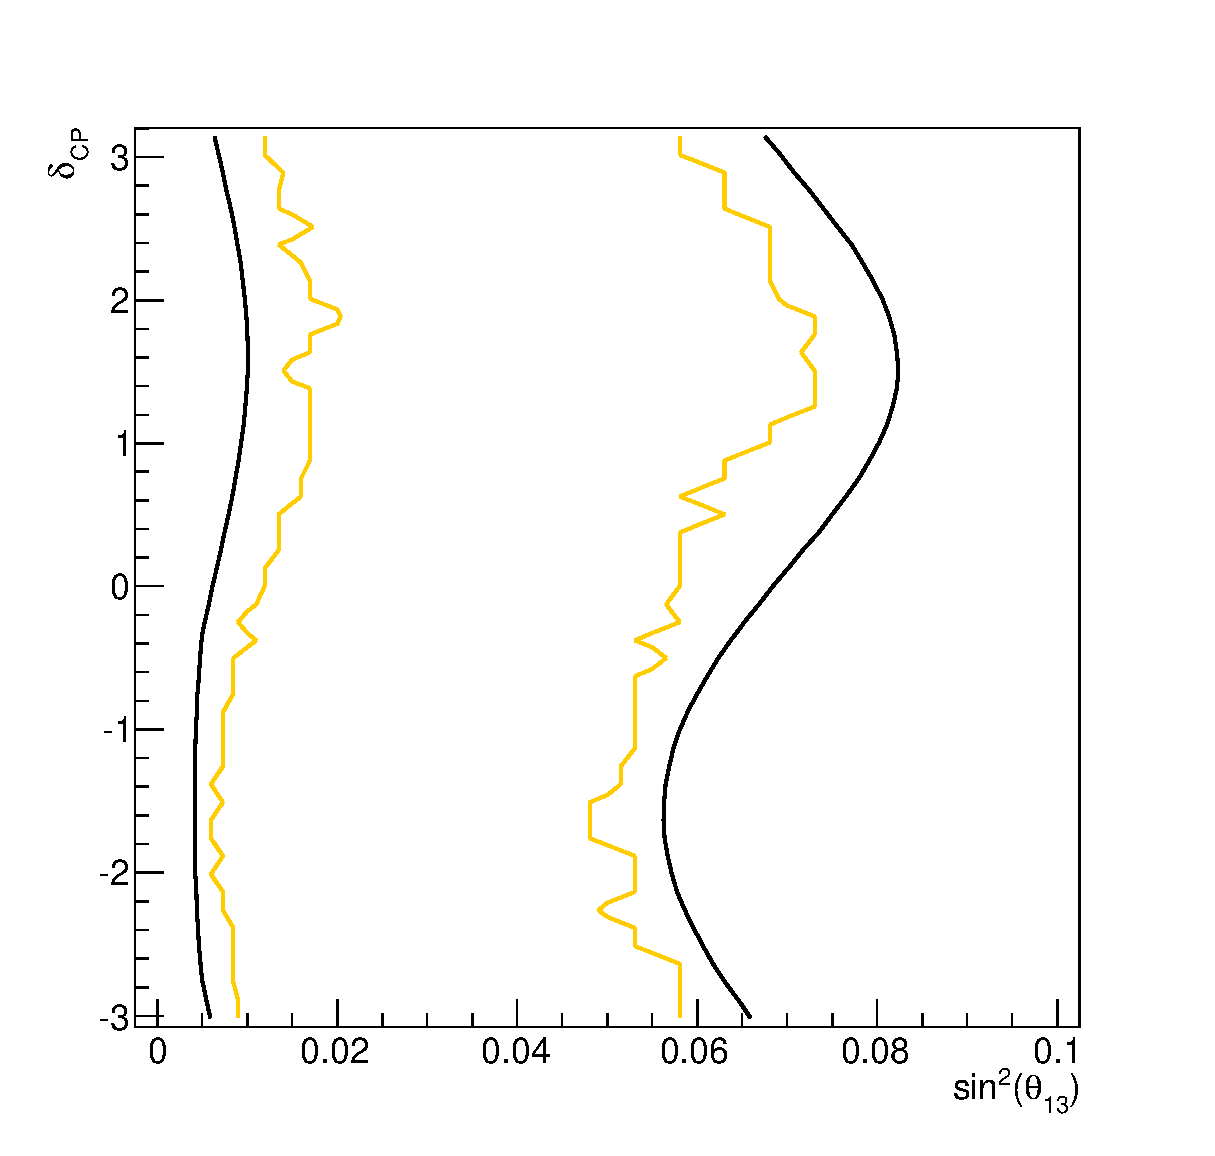
\includegraphics[width=18pc]{./images/appendix/sensitivity_studies/sensitivity_data_ih_chisq_vs_theta13_deltacp_with_datafit.eps}
\caption {
 90\% CL region in ($\sin^{2}\theta_{13}$, $\delta_{CP}$) space for the best fit point found 
  for Run1+2+3 with Normal Hierarchy.
  Orange line is the sensitivity contour that was computed by averaging
  the contours of the ensemble of hundreds of toy MC experiments and,
  for each experiment, it was minimized with respect to 
  $\sin^{2}\theta_{13}$, $\delta_{CP}$
  and all relevant nuisance parameters for the joint analysis.
Black line is the result of the Run1+2+3 dataset fit. 	
  }
\label{fig:sensitivity:data:confreg_sinsqtheta13_deltacp_ih}
\end{minipage}
\hspace{0.03\linewidth}
\begin{minipage}[t]{0.48\linewidth}
\center
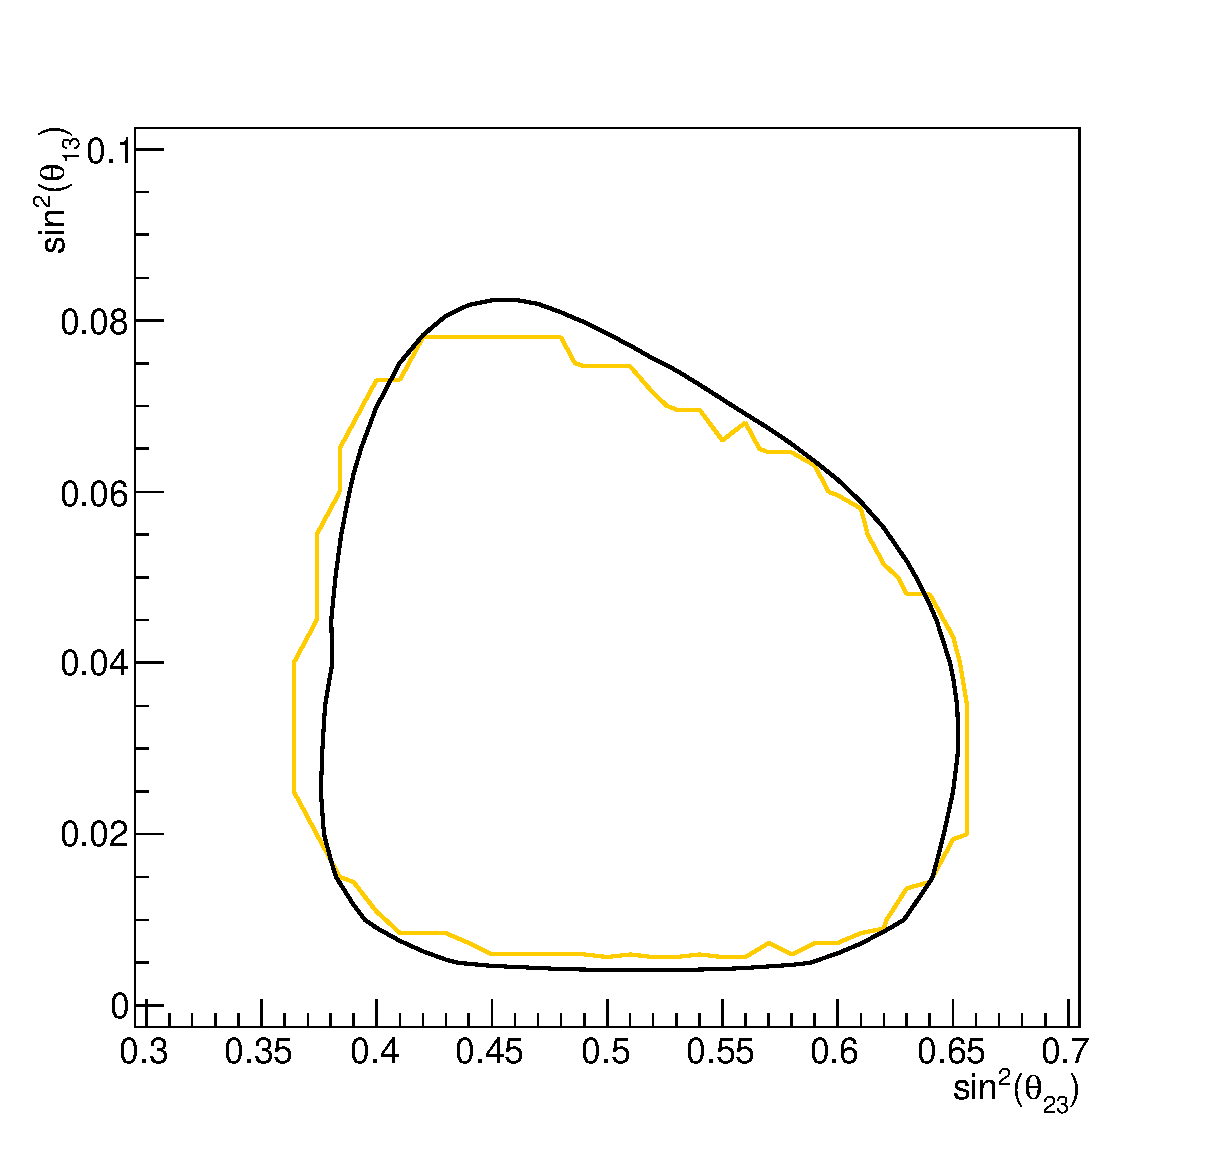
\includegraphics[width=18pc]{./images/appendix/sensitivity_studies/sensitivity_data_ih_theta13_theta23_with_datafit.eps}
\caption {
 90\% CL region in ($\sin^{2}\theta_{23}$, $\sin^{2}\theta_{13}$) space for the best fit point found 
  for Run1+2+3 with Normal Hierarchy.
  Orange line is the sensitivity contour that was computed by averaging
  the contours of the ensemble of hundreds of toy MC experiments and,
    for each experiment, it was minimized with respect to 
  $\sin^{2}\theta_{13}$, $\delta_{CP}$
  and all relevant nuisance parameters for the joint analysis.
Black line is the result of the Run1+2+3 dataset fit. 
}
\label{fig:sensitivity:data:confreg_sinsqtheta23_sinsqtheta13_ih}
\end{minipage}


\end{figure*}

